\documentclass[hyperref={pdfpagelabels=false}]{beamer}
% beamer already loads hyperref; do NOT load \usepackage{hyperref} again.

\usepackage{ragged2e} % 文字向兩邊對齊
\renewcommand{\raggedright}{\leftskip=0pt \rightskip=0pt plus 0cm}

\usepackage{listings}
\usepackage{lmodern}
\usepackage{fontspec}
\usepackage{xeCJK}
\setCJKmainfont{Noto Sans CJK TC}
%（可選）若你會用到無襯線中文或等寬中文，建議補上：
\setCJKsansfont{Noto Sans CJK TC}
\setCJKmonofont{Noto Sans Mono CJK TC}

\usepackage[english]{babel}
\usepackage{amsmath,amssymb,amsfonts,amsthm}

% hyperref settings (since beamer already loads hyperref)
\hypersetup{
  colorlinks=true,
  urlcolor=blue,
  citecolor=blue,
  pdfborder={0 0 0}
}

\usepackage{accsupp}% http://ctan.org/pkg/accsupp
\newcommand{\emptyaccsupp}[1]{\BeginAccSupp{ActualText={}}#1\EndAccSupp{}}

\usepackage{tikz}
\usetikzlibrary{arrows,decorations.pathmorphing,backgrounds,fit,positioning,shapes.symbols,chains}

\usepackage{booktabs}
\usepackage{threeparttable}
\usepackage{colortbl} 
\usepackage{xcolor}
\usetikzlibrary{tikzmark}

\newcommand{\indep}{\perp\!\!\!\perp}
\newcommand{\nindep}{\not\!\perp\!\!\!\perp}

\beamertemplatefootpagenumber


\usepackage{listings}
%%%%%%%%%%%%%%%%%%%%%%%%%%%%%%%%%%%%%%%%%%%%%%%%%%%%%%%%%%%%%%%%%%%%%%%%%%%%%%
% LaTeX snippet: language and style definition of Stata for listings package.
%                [listings](http://www.ctan.org/pkg/listings) 
%                [Stata](http://www.stata.com/)
%
% Usage:
%     Copy the code into your preamble, or import it by `\include` .
%     then in your doc:
%     \lstinputlisting[style=numbers]{DO-SCRIPT}
%     \lstinputlisting[style=numbers, style=stata-editor]{DO-SCRIPT}
%     \lstinputlisting[style=nonumbers, frame=none]{DO-SCRIPT}
% How it works:
%     - The language is defined by `\lstdefinelanguage{Stata}`
%     - Four styles is defined by `\lstdefinestyle{STYLE-NAME}`, 
%       they are: numbers and no numbers, plain(black and white) and colorful
%       (colored roughly like stata editor.)
% Tips:
%     - Generally you only need to set your default in the last part,
%       that is, code inside of `\lstset`.
%     - Add more keywords(I can not list all of them) in the `\lstset` part.
%     - Do NOT leave any blank lines in commands
%       (`\lstddefinelanguage', `\lstdefinestyle` and `\lstset`)
%
% update: 2014-04-16
% version: 0.1
% author: kongs
% licence: MIT
% url: https://gist.github.com/kongs-sublime/10862838
%
% TODO: 
%       - finish keyword list.
%       - precise colors that match stata editor?
%       - make it flexible(fonts and style)
%
%%%%%%%%%%%%%%%%%%%%%%%%%%%%%%%%%%%%%%%%%%%%%%%%%%%%%%%%%%%%%%%%%%%%%%%%%%%%%%


% langugae defination
\lstdefinelanguage{Stata}{
	% Left for users to add missing commands,
	% with possibility of choosing different style.
	morekeywords=,
	% Popular add-on commands
	morekeywords=[2]{cntrade, chinafin, 
		wbopendata, spmap,
	},
	% System commands
	morekeywords=[3]{regress, summarize, 
		display,
	},
	% Keywords
	morekeywords=[4]{forvalues, if, foreach, set},
	% Built-in functions
	morekeywords=[5]{rnormal, runiform},
	morecomment=[l]{//},
	% morecomment=[l]{*},  // `*` maybe used as multiply operator. So use `//` as line comment.
	morecomment=[s]{/*}{*/},
	% morecomment=[s]{,}{//},
	% The following is used by macros, like `lags'.
	morecomment=[n][keywordstyle9]{`}{'},
	morestring=[b]",
	sensitive=true,
}

\lstdefinestyle{numbers}{
	numbers=left, 
	stepnumber=1, 
	numberstyle=\tiny\emptyaccsupp,
	xleftmargin=2em,
}

\lstdefinestyle{nonumbers}{
	numbers=none,
}

\lstdefinestyle{stata-plain}{
	language=Stata,
	basicstyle=\footnotesize\ttfamily,
}

\lstdefinestyle{stata-editor}{
	language=Stata,
	basicstyle=\footnotesize\ttfamily,  
	keywordstyle={\color{NavyBlue}},  
	keywordstyle=[2]{\color{NavyBlue}},
	keywordstyle=[3]{\color{NavyBlue}},
	keywordstyle=[4]{\color{NavyBlue}},
	keywordstyle=[5]{\color{Blue}},
	keywordstyle=[9]{\color{TealBlue}},
	stringstyle=\color{Maroon},
	commentstyle=\color{OliveGreen},
}

\lstset{
	language=Stata,
	style=stata-plain,
	% style=stata-editor,
	style=numbers,
	showstringspaces=false,
	breaklines,
	frame=single,
	% To add missing commands
	% morekeywords={xtreg, xtunitroot},
}




\title[]  
{Instrumental Variables Design}

%\subtitle
%{免除部分負擔對幼兒醫療利用與健康的影響:斷點迴歸分析}

%\author 
 %{Tzu-Ting Yang\inst{1} \and Hsing-Wen Han\inst{2} \and Hsien-Ming Lien\inst{3}}

%\institute[short]{\inst{1} Academia Sinica \and \inst{2} Tamkang University \and \inst{3} National Chengchi University}


\author 
{Prof. Tzu-Ting Yang  \\ 楊子霆}

%\institute{Institute of Economics, Academia Sinica  \\ Econ, NTU}
\institute{Institute of Economics, Academia Sinica  \\ 中央研究院經濟研究所}
%\institute{Institute of Economics, Academia Sinica  \\ Econ, NTU}
%\institute{Institute of Economics, Academia Sinica  \\ IMES/IDAS, NCCU}

%\author 
%{楊子霆 \\ 中研院經濟所}

%\institute 
%{中正大學國際經濟專題研討}




\date
{\today}


% \usetheme{CambridgeUS}
% %\usecolortheme{seahorse}
% \setbeamertemplate{footline}{%
% 	\hfill\usebeamercolor[fg]{page number in head/foot}%
% 	\usebeamerfont{page number in head/foot}%
% 	\insertframenumber\,/\,\inserttotalframenumber\hspace{1em}\vspace{2pt}%
% }

% \usetheme{Boadilla}
% %\useinnertheme{rectangles}

% %\usetheme{CambridgeUS}
% \usecolortheme{seahorse}
% \setbeamertemplate{footline}{%
% 	\hfill\usebeamercolor[fg]{page number in head/foot}%
% 	\usebeamerfont{page number in head/foot}%
% 	\insertframenumber\,/\,\inserttotalframenumber\hspace{1em}\vspace{2pt}%
% }


%\usepackage{beamerthemeshadow}
%\usecolortheme{seahorse}
\setbeamertemplate{footline}{%
	\hfill\usebeamercolor[fg]{page number in head/foot}%
	\usebeamerfont{page number in head/foot}%
	\insertframenumber\,/\,\inserttotalframenumber\hspace{1em}\vspace{2pt}%
}


%\usepackage{beamerthemeshadow}

\beamersetuncovermixins{\opaqueness<1>{25}}{\opaqueness<2->{15}}

\begin{document}


\begin{frame}{}
 \titlepage
\end{frame}




\title[]  
{Main Idea}


\author 
{}

%\institute{Institute of Economics, Academia Sinica  \\ Econ, NTU}
%\institute{Institute of Economics, Academia Sinica  \\ IMES/IDAS, NCCU}
\institute{}

%\author 
%{楊子霆 \\ 中研院經濟所}

%\institute 
%{中正大學國際經濟專題研討}




\date
{}


\begin{frame}{}
	\titlepage
\end{frame}



\begin{frame}{Main Idea of Instrumental Variables}
	
	\begin{itemize}
		\item The Instrumental Variable (IV) is an exogenous sources of
		variation that drives the treatment $D_{i}$ but unrelated to other confounding factors that affect outcome $Y_{i}$
		\vspace{0.2cm}
		\item Intuitively, IV breaks variation of the treatment $D_{i}$ into two parts
				\vspace{0.2cm}
		\begin{itemize}
			\item[1] A part that might be correlated with other confounding factors 
			\vspace{0.2cm}
			\begin{itemize}		
			\item This part causes selection bias
						\vspace{0.2cm}
					\end{itemize}
			\item[2] A part that is not
			\vspace{0.2cm}
			\begin{itemize}		
				\item This part could represent the clean causal effect
			\end{itemize}
			
		\end{itemize}
		\vspace{0.2cm}
	\item Use the variation in  $D_{i}$ that is not correlated with other confounding factors  to estimate causal effect of the treatment 
		
		%By isolating the part that is not correlated with $u_{i}$, IV use this variation to estimate causal effect of the treatment $D_{i}$
		
		%use these to estimate
		%\item We need more powerful tools or better data to eliminate selection bias from unobservable omitted variable 
	\end{itemize}
\end{frame}





\begin{frame}{Unobservable Omitted Variable}
	
	\begin{itemize}
		\item Suppose the true model is:
		
		\begin{align*}
		\mathrm{Y}_i &= \delta + \alpha D_i + \beta_{1} X_{i} + \beta_{2} U_{i} + \epsilon_{i}
		\end{align*}
		
		\vspace{0.3cm}
		\item $X_{i}$ is the \textbf{observed characteristics} 
		\vspace{0.3cm}
		\begin{itemize}
			\item We can directly control for it
		\end{itemize}
				\vspace{0.3cm}
		\item But $U_{i}$ is the \textbf{unobserved characteristics} 
				\vspace{0.3cm}
			\begin{itemize}
		\item e.g. ability, preference, health
			\end{itemize}
		\vspace{0.3cm}
		\item So we cannot include it into our regression and estimate the following model:
		\begin{align*}
		\mathrm{Y}_i &= \delta + \alpha D_i + \beta_{1} X_{i} + \zeta_i
		\end{align*}
		\item where $\zeta_i = \beta_{2} U_{i} + \epsilon_{i}$
		
	\end{itemize}
	
\end{frame}




\begin{frame}{Unobservable Omitted Variable}
	
	\begin{itemize}
		\item As mentioned before, failure to include key covariates will lead to omitted variable bias
		\begin{equation*}
		\begin{aligned}
		\hat{\alpha} &\overset{p}{\rightarrow} \alpha + \dfrac{Cov(\zeta_{i},D_{i})}{V(D_{i})}  \\	
		&= \alpha + \beta_{2} \dfrac{Cov(U_{i},D_{i})}{V(D_{i})}
		\end{aligned}	
		\end{equation*}
		
		
		\item Remember there is NO omitted variable bias (OVB) if:
		\vspace{0.2cm}
		\begin{itemize}
			\item[1] $U_{i}$ is unrelated to $Y_{i}$: $\beta_{2}=0$
			\vspace{0.2cm} 
			\item[2] $U_{i}$ is unrelated to $D_{i}$: $Cov(U_{i},D_{i})=0$
			\vspace{0.2cm}
		\end{itemize}
		\item To obtain eliminate OVB, we need a variation in $D_{i}$ that is unrelated to the unobserved confounding factor $U_{i}$
		
		
	\end{itemize}
	
\end{frame}




\begin{frame}{Main Idea of Instrumental Variables}

	\begin{figure}
		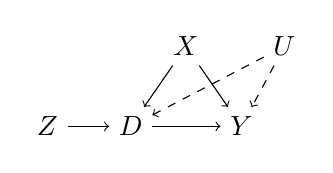
\begin{tikzpicture}[comment/.style={rectangle, text centered}]
			\centering
			
			\node (u) {$X$};
			\node (U) [right=2em of u] {$U$}; 
			\node (D) [below=1.5em of u, xshift=-2em] {$D$};
			\node (Z) [left=1.5em of D] {$Z$};
			\node (Y) [below=1.5em of u, xshift=2em] {$Y$};
			
			\draw [->,solid] (u) -- node [auto]{} (D);
			\draw [->,solid] (u) --  node [auto, swap]{} (Y);
			\draw [->,dashed] (U) -- node [auto, swap]{} (D);
			\draw [->,dashed] (U) -- node [auto]{}(Y);
			\draw [->] (D) -- node [auto]{} (Y);
			\draw [->] (Z) -- node [auto]{} (D);
			
			%\draw[<->, >=latex', shorten >=2pt, shorten <=2pt, bend right=30, thick, color=red]
			%(Z.south) to node[auto, swap] {exclusion restriction}(Y.south);
			% \node [comment, below = 0.08 of D] (1) {\Large\color{red}$\times$};
			
		\end{tikzpicture}
	\end{figure}
	\begin{itemize}
		\item $Y$ is an outcome (e.g. earnings), 
		\vspace{0.2cm}
		\item $Z$ is the instrument
		\vspace{0.2cm} 
		\item $D$ is the treatment (e.g. college degree)
		\vspace{0.2cm}
		\item $X$ is the \textbf{observed} confounding factor (e.g. family income)
		\vspace{0.2cm}
		\item $U$ is the \textbf{unobserved} confounding factor (e.g. ability)
	\end{itemize}
\end{frame}





\begin{frame}{Main Idea of Instrumental Variables}
	\begin{figure}
	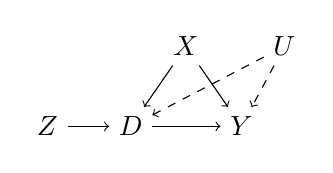
\begin{tikzpicture}[comment/.style={rectangle, text centered}]
		\centering
		
		\node (u) {$X$};
		\node (U) [right=2em of u] {$U$}; 
		\node (D) [below=1.5em of u, xshift=-2em] {$D$};
		\node (Z) [left=1.5em of D] {$Z$};
		\node (Y) [below=1.5em of u, xshift=2em] {$Y$};
		
		\draw [->,solid] (u) -- node [auto]{} (D);
		\draw [->,solid] (u) --  node [auto, swap]{} (Y);
		\draw [->,dashed] (U) -- node [auto, swap]{} (D);
		\draw [->,dashed] (U) -- node [auto]{}(Y);
		\draw [->] (D) -- node [auto]{} (Y);
		\draw [->] (Z) -- node [auto]{} (D);
		
		%\draw[<->, >=latex', shorten >=2pt, shorten <=2pt, bend right=30, thick, color=red]
		%(Z.south) to node[auto, swap] {exclusion restriction}(Y.south);
		% \node [comment, below = 0.08 of D] (1) {\Large\color{red}$\times$};
		
	\end{tikzpicture}
\end{figure}
	\begin{itemize}
		\item  \textbf{Unobserved ability} $U$ might confound with the effect of college degree $D$ 
		\vspace{0.2cm}
		\begin{itemize}
			\item Since ability affects people to get college degree $D$ and their earnings $Y$
			\vspace{0.2cm}
		\end{itemize}
		\item We need to find an IV that generate a variation in getting college degree $D$ that is unrelated to ability  $U$
		
		
	\end{itemize}
\end{frame}





\begin{frame}{Main Idea of Instrumental Variables}
	\begin{figure}
	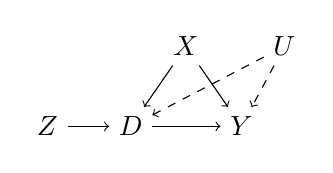
\begin{tikzpicture}[comment/.style={rectangle, text centered}]
		\centering
		
		\node (u) {$X$};
		\node (U) [right=2em of u] {$U$}; 
		\node (D) [below=1.5em of u, xshift=-2em] {$D$};
		\node (Z) [left=1.5em of D] {$Z$};
		\node (Y) [below=1.5em of u, xshift=2em] {$Y$};
		
		\draw [->,solid] (u) -- node [auto]{} (D);
		\draw [->,solid] (u) --  node [auto, swap]{} (Y);
		\draw [->,dashed] (U) -- node [auto, swap]{} (D);
		\draw [->,dashed] (U) -- node [auto]{}(Y);
		\draw [->] (D) -- node [auto]{} (Y);
		\draw [->] (Z) -- node [auto]{} (D);
		
		%\draw[<->, >=latex', shorten >=2pt, shorten <=2pt, bend right=30, thick, color=red]
		%(Z.south) to node[auto, swap] {exclusion restriction}(Y.south);
		% \node [comment, below = 0.08 of D] (1) {\Large\color{red}$\times$};
		
	\end{tikzpicture}
\end{figure}
	\begin{itemize} 
		\item IV initiates a causal chain: the instrument $Z$ affects $D$, which in turn affects $Y$
		\vspace{0.2cm}
		\item A valid IV needs to satisfy the following conditions:
		\vspace{0.2cm}
		\begin{itemize} 
			\item[1] First-stage relationship (Instrument relevance): $Z$ affects $D$
			
		\end{itemize}
		
		
	\end{itemize}
\end{frame}






\begin{frame}{Main Idea of Instrumental Variables}
	\begin{figure}
		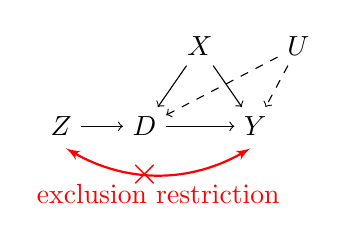
\begin{tikzpicture}[comment/.style={rectangle, text centered}]
		\centering
			\node (u) {$X$};
		\node (U) [right=2em of u] {$U$}; 
		\node (D) [below=1.5em of u, xshift=-2em] {$D$};
		\node (Z) [left=1.5em of D] {$Z$};
		\node (Y) [below=1.5em of u, xshift=2em] {$Y$};
		
		\draw [->,solid] (u) -- node [auto]{} (D);
		\draw [->,solid] (u) --  node [auto, swap]{} (Y);
		\draw [->,dashed] (U) -- node [auto, swap]{} (D);
		\draw [->,dashed] (U) -- node [auto]{}(Y);
		\draw [->] (D) -- node [auto]{} (Y);
		\draw [->] (Z) -- node [auto]{} (D);
		\draw[<->, >=latex', shorten >=2pt, shorten <=2pt, bend right=30, thick, color=red] 
		(Z.south) to node[auto, swap] {exclusion restriction}(Y.south);
		\node  [comment, below = 0.08 of D] (1) {\Large\color{red}$\times$};
		\end{tikzpicture}
	\end{figure}
	\begin{itemize} 
		
		\item A valid IV needs to satisfy the following conditions:
		\vspace{0.2cm}
		\begin{itemize} 
			\item[2] Exclusion restriction (Instrument exogeneity):
			\begin{itemize} 
				\vspace{0.2cm}
				\item \textbf{No direct or indirect effect} of the instrument $Z$ on the outcome $Y$ NOT through the treatment variable $D$
				\vspace{0.2cm}
				\item The instrument $Z$ affects the outcome $Y$ \textbf{only through the treatment variable $D$}
			\end{itemize}
			
		\end{itemize}
		
	\end{itemize}
\end{frame}







\begin{frame}{Main Idea of Instrumental Variables}
	\begin{figure}
	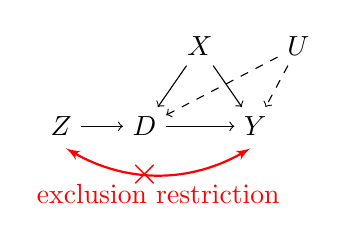
\begin{tikzpicture}[comment/.style={rectangle, text centered}]
		\centering
		\node (u) {$X$};
		\node (U) [right=2em of u] {$U$}; 
		\node (D) [below=1.5em of u, xshift=-2em] {$D$};
		\node (Z) [left=1.5em of D] {$Z$};
		\node (Y) [below=1.5em of u, xshift=2em] {$Y$};
		
		\draw [->,solid] (u) -- node [auto]{} (D);
		\draw [->,solid] (u) --  node [auto, swap]{} (Y);
		\draw [->,dashed] (U) -- node [auto, swap]{} (D);
		\draw [->,dashed] (U) -- node [auto]{}(Y);
		\draw [->] (D) -- node [auto]{} (Y);
		\draw [->] (Z) -- node [auto]{} (D);
		\draw[<->, >=latex', shorten >=2pt, shorten <=2pt, bend right=30, thick, color=red] 
		(Z.south) to node[auto, swap] {exclusion restriction}(Y.south);
		\node  [comment, below = 0.08 of D] (1) {\Large\color{red}$\times$};
	\end{tikzpicture}
\end{figure}
	\begin{itemize}
		\item We can test whether the \textbf{instrument relevance} is satisfied 
		\vspace{0.2cm}
		\item But the \textbf{instrument exogeneity} cannot be tested
		\vspace{0.2cm}
		
			\begin{itemize}
		\item You have to convince your audience that it is satisfied
		
			\end{itemize}
	\end{itemize}
\end{frame}



\title[]  
{Identification}


\author 
{}

%\institute{Institute of Economics, Academia Sinica  \\ Econ, NTU}
%\institute{Institute of Economics, Academia Sinica  \\ IMES/IDAS, NCCU}
\institute{}

%\author 
%{楊子霆 \\ 中研院經濟所}

%\institute 
%{中正大學國際經濟專題研討}




\date
{}


\begin{frame}{}
	\titlepage
\end{frame}





\begin{frame}{Example}{Effect of Military Service on Lifetime Income}
	
	
Joshua D. Angrist (1990) ``\textbf{Lifetime Earnings and the Vietnam Era Draft Lottery: Evidence from Social Security Administrative Records}" AER
	
	
	\begin{itemize}
		\item He wanted to examine the effect of military service on lifetime income.	
		\vspace{0.2cm}	
		\item We will use Angrist's paper on the effects of military service ($D_{i}$) on earnings ($Y_{i}$) as an example to go through key concept of IV design
		
		
	\end{itemize}
\end{frame}





\begin{frame}{Example}{Effect of Military Service on Lifetime Income}
	\begin{itemize}
		\item Joining military service is a personal choice
		\vspace{0.2cm}
		\item Is there any selection bias due to \textbf{unobservable confounding factors} in this example ?
		\vspace{0.2cm}
		\begin{itemize}
			\item \textbf{Time preference:} 
			\begin{itemize}	
				\vspace{0.2cm}
				\item Less patient people may voluntarily join military service early
				\vspace{0.2cm}
				\item This myopic thinking may have negative impact on their earnings (e.g. less human capital investment) 
				\vspace{0.2cm} 
			\end{itemize}	
			\item \textbf{Health condition:} 
			\vspace{0.2cm} 
			\begin{itemize}	
				\item Better health people can join military service 
				\vspace{0.2cm} 
				\item Better health condition also have positive impact on their earnings
			\end{itemize}			
		\end{itemize}
		\vspace{0.2cm} 
		\item We need a IV for the treatment variable of joining military service
		
	\end{itemize}
\end{frame}







\begin{frame}{Example}{Effect of Military Service on Lifetime Income}
	
	\begin{itemize}
		\item Angrist (1990) uses the \textbf{Vietnam draft lottery} ($Z_{i}$) as in IV for military service
		\vspace{0.3cm} 
			\begin{itemize}
		\item In the 1960s and early 1970s, young American men were draft for military service to serve in Vietnam
		\vspace{0.3cm} 
		\item Concerns about the fairness of the conscription policy lead to the introduction of a \textbf{draft lottery} in 1970
		% \vspace{0.3cm} 
		%\item A promising IV for serving military is therefore draft eligibility
		%\vspace{0.3cm} 
		%\item Since this was determined by a lottery over birthdays
			\end{itemize}
		
		
		
	\end{itemize}
\end{frame}


\begin{frame}{Example}{Effect of Military Service on Lifetime Income}
	\begin{itemize}
		\item From 1970 to 1972 \textbf{random sequence numbers} were assigned to each birth date in cohorts of 19-year-olds 
		\vspace{0.2cm} 
			\begin{itemize}
		\item Men with lottery numbers below a cutoff were eligible for military service 
				\vspace{0.2cm} 
		\item While men with numbers above the cutoff were ineligible
		\vspace{0.2cm} 
							\begin{itemize}		
		\item $Z=\mathbf{I}[L<c]$
				\vspace{0.2cm} 

				\item $L$ is lottery number and $c$ is cutoff	
								\vspace{0.2cm} 	
			\end{itemize} 
		\end{itemize} 	
		\item The eligibility did NOT perfectly determinate military service:
		\vspace{0.2cm}
		\begin{itemize} 
			\item Many draft-eligible men were exempted for health and other reasons
			\vspace{0.2cm}
			\item Draft-ineligible men volunteered for service
			\vspace{0.2cm}
			
		\end{itemize} 
		\item Next, we briefly discuss whether draft eligibility induced by lottery is a good IV or not
		
	\end{itemize}
\end{frame}






\begin{frame}{Example}{Effect of Military Service on Lifetime Income}
	\begin{itemize}
		\item The lottery used by the Selective Service to determine who would be drafted for Vietnam first
	\end{itemize}
	\begin{center}
		\begin{figure}[p]
			\centering
			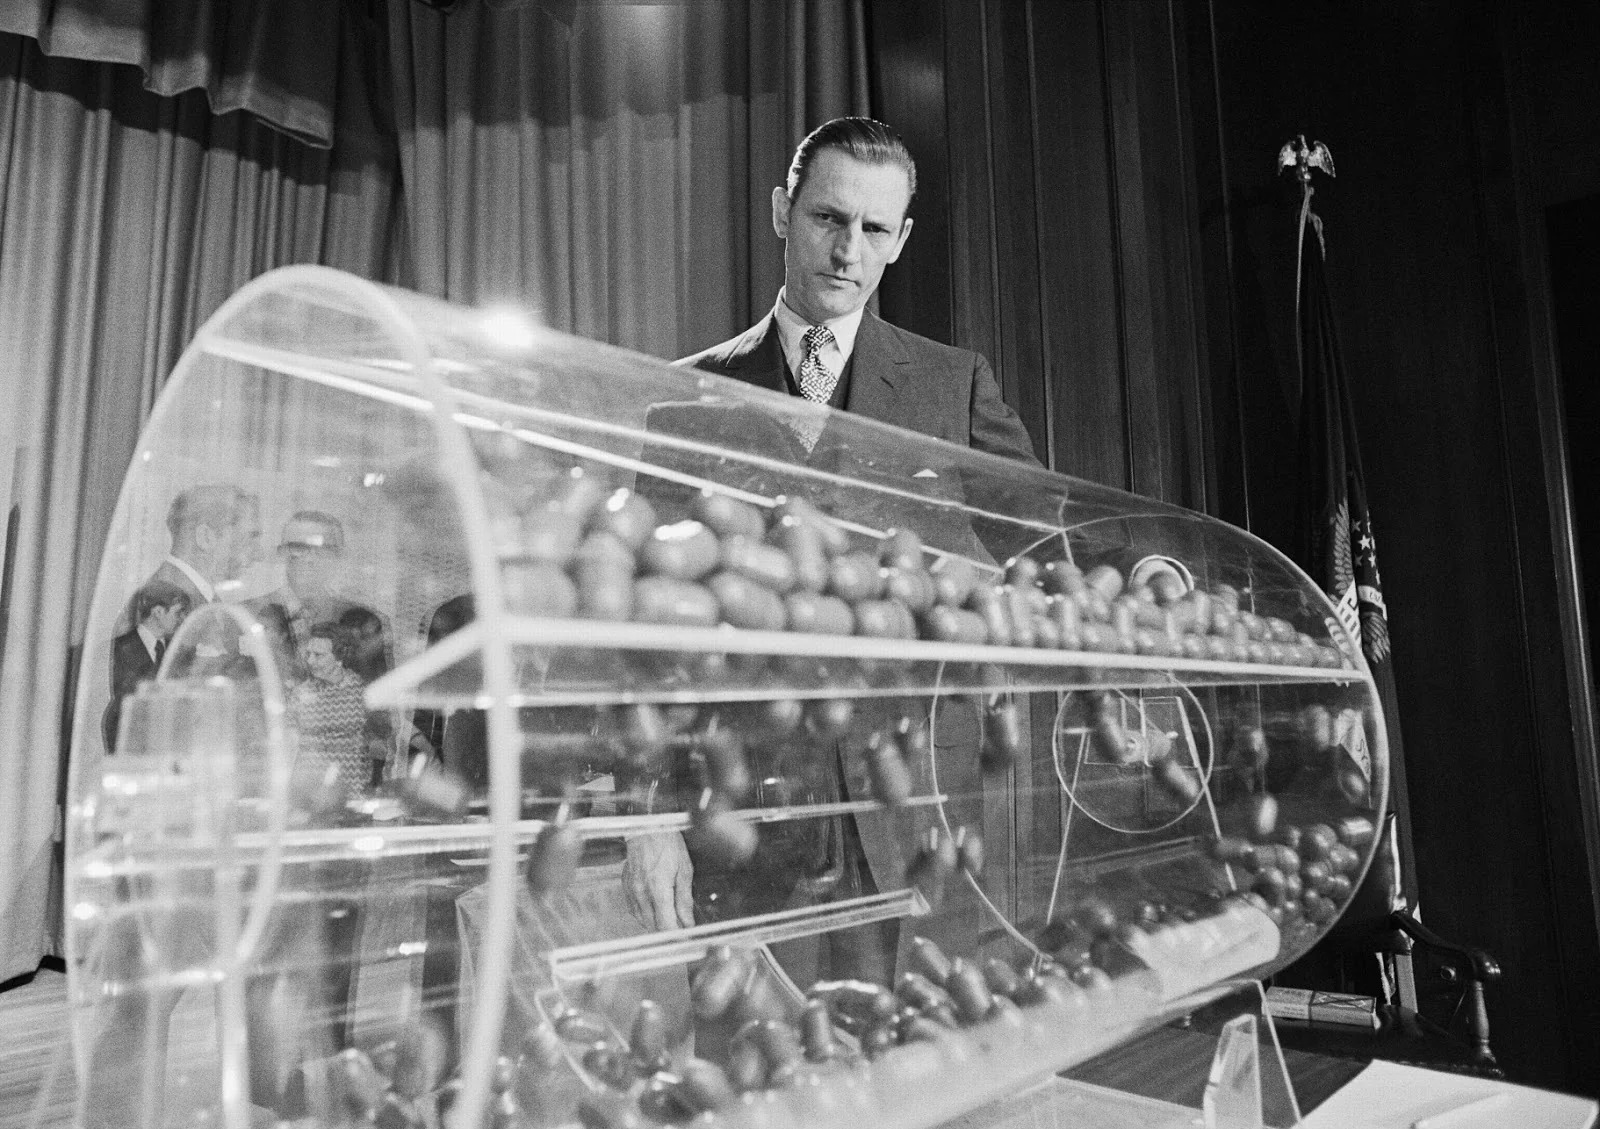
\includegraphics[width=0.7\textwidth]{figure/IV_lottery.jpg}
			\begin{minipage}{0.9\linewidth}
			\fontsize{8}{8pt}\selectfont
			\emph{Source:} Historic Photographs
		\end{minipage}	
			
		\end{figure}
	\end{center}
\end{frame}






\begin{frame}{Example}{Effect of Military Service on Lifetime Income}
	\begin{itemize}
		
		\item First-stage relationship (Instrument relevance): $Z_{i}$ affects $D_{i}$
		\vspace{0.2cm}
		\begin{itemize}
			\item Vietnam veteran status (joining military service) was not completely determined by randomized draft eligibility
			\vspace{0.2cm}
			\item But draft eligibility is highly correlated with Vietnam veteran status
			\vspace{0.2cm}
		\end{itemize} 
		\item Exclusion restriction (Instrument exogeneity):
		\vspace{0.2cm}
		\begin{itemize}
			\item The draft eligibility is determined by random numbers
			\vspace{0.2cm}
			\item These numbers should not affect one's earnings directly
		\end{itemize} 
		%\vspace{0.2cm}
		%\item Independent assumption (Instrument exogeneity):
		% \vspace{0.2cm}
		%\begin{itemize}
		%\item Draft eligibility should not be correlated to other confounding factors that affect earnings
		%\end{itemize}  
		
		
	\end{itemize}
\end{frame}




\begin{frame}{Potential Outcomes Framework}
	\begin{itemize}
		
		\item \textcolor{blue}{Treatment Assignment}
		\begin{align*}
		Z_{i}=\left\lbrace
		\begin{array}{l}
		1\quad \text{if an individual $i$ is eligible for a treatment}\\
		0\quad \text{if an individual $i$ is not eligible for a treatment}
		\end{array}\right.
		\end{align*}
		\begin{itemize}
			\item $Z_{i}=1$: those who get draft eligibility 
				\vspace{0.2cm}
				\item $Z_{i}=0$: those who do not get draft eligibility 		
						\vspace{0.2cm}
					\begin{itemize}
			\item Due to lottery results
						\end{itemize}
			
		
			\vspace{0.2cm}
		\end{itemize}
		
	\end{itemize}
\end{frame}




\begin{frame}{Potential Outcomes Framework}
	\begin{itemize}
		
		\item \textcolor{blue}{Potential Treatments}
		\vspace{0.2cm}
		\begin{itemize}
			\item $\mathrm{D}^{z}_{i}$: Potential treatment status given the value of $Z$
			\vspace{0.2cm}
					\begin{itemize}
			\item $\mathrm{D}^{1}_{i}$: Potential treatment status if eligible for a treatment 
						\vspace{0.2cm}
					
			\vspace{0.2cm}
			\item $\mathrm{D}^{0}_{i}$: Potential treatment status if not eligible for a treatment 
			\vspace{0.2cm}
					\end{itemize}
			
		\end{itemize}
		\vspace{0.2cm}
		\item \textcolor{blue}{Observed Treatment}
		\begin{align*}
		D_{i}=\left\lbrace
		\begin{array}{l}
		\mathrm{D}^{1}_{i}\quad \text{if $Z_{i}=1$} \\
		\mathrm{D}^{0}_{i}\quad \text{if $Z_{i}=0$}
		\end{array}\right
		\end{align*}
		\item or, in a more compact notation: 
		$\mathrm{D}_{i}=Z_{i}\mathrm{D}^{1}_{i}+(1-Z_{i})\mathrm{D}^{0}_{i} $
		
	\end{itemize}
\end{frame}












\begin{frame}{Potential Outcomes Framework}
	
	
	
	\begin{itemize}
		
		\item \textcolor{blue}{Potential Outcomes}
					\vspace{0.2cm}
		\begin{itemize}
			\item $\mathrm{Y}^{1}_{i}$: outcome if an individual $i$ get treatment 
					\vspace{0.2cm}
				\begin{itemize}	
			\item Either $\mathrm{D}^{1}_{i}=1$ or $\mathrm{D}^{0}_{i}=1$
			\vspace{0.2cm}
					\end{itemize}
			\item $\mathrm{Y}^{0}_{i}$: outcome if an individual $i$ does not get treatment 
			\vspace{0.2cm}
			\begin{itemize}	
			\item Either $\mathrm{D}^{0}_{i}=0$ or $\mathrm{D}^{1}_{i}=0$
								\end{itemize}
		\end{itemize}
		\vspace{0.2cm}
		\item \textcolor{blue}{Observed Outcomes}
		\begin{align*}
		Y_{i}=\left\lbrace
		\begin{array}{l}
		\mathrm{Y}^{1}_{i}\quad \text{if $\mathrm{D}^{1}_{i}=1$ or $\mathrm{D}^{0}_{i}=1$} \\
		\mathrm{Y}^{0}_{i}\quad \text{if $\mathrm{D}^{0}_{i}=0$ or $\mathrm{D}^{1}_{i}=0$}
		\end{array}\right
		\end{align*}
		\item or, in a more compact notation: 
		$\mathrm{Y}_{i}=D^{z}_{i}\mathrm{Y}^{1}_{i}+(1-D^{z}_{i})\mathrm{Y}^{0}_{i} $
		
	\end{itemize}
\end{frame}


\begin{frame}{Identification Results for IV}
	\begin{figure}
	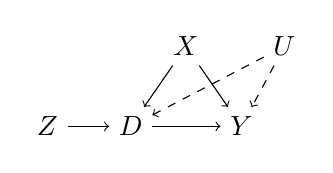
\begin{tikzpicture}[comment/.style={rectangle, text centered}]
		\centering
		
		\node (u) {$X$};
		\node (U) [right=2em of u] {$U$}; 
		\node (D) [below=1.5em of u, xshift=-2em] {$D$};
		\node (Z) [left=1.5em of D] {$Z$};
		\node (Y) [below=1.5em of u, xshift=2em] {$Y$};
		
		\draw [->,solid] (u) -- node [auto]{} (D);
		\draw [->,solid] (u) --  node [auto, swap]{} (Y);
		\draw [->,dashed] (U) -- node [auto, swap]{} (D);
		\draw [->,dashed] (U) -- node [auto]{}(Y);
		\draw [->] (D) -- node [auto]{} (Y);
		\draw [->] (Z) -- node [auto]{} (D);
		
		%\draw[<->, >=latex', shorten >=2pt, shorten <=2pt, bend right=30, thick, color=red]
		%(Z.south) to node[auto, swap] {exclusion restriction}(Y.south);
		% \node [comment, below = 0.08 of D] (1) {\Large\color{red}$\times$};
		
	\end{tikzpicture}
\end{figure}
	
	
	\begin{itemize}
		\item The IV method characterize a causal chain reaction leading from the instrument $Z_{i}$ (draft eligibility) to outcome $Y_{i}$ (earnings)
		\vspace{0.2cm}
		\item Intuitively:
		\begin{equation*}
		\begin{aligned}
		& \text{Effect of instrument on outcome} \\ 
		&=	(\text{Effect of instrument on treatment}) \\
		&\times (\text{Effect of treatment on outcome})
		\end{aligned}
		\end{equation*}
		
		
	\end{itemize}
\end{frame}





\begin{frame}{Identification Results for IV}
	\begin{itemize}
		
		\item Rearranging, the causal effect of military service on earnings is:
		\begin{equation*}
			\begin{aligned}
				& \text{Effect of treatment on outcome} \\ 
				&= \dfrac{\text{Effect of instrument on outcome}}{\text{Effect of instrument on treatment}}
			\end{aligned}
		\end{equation*}
		\item Formal representation:
		\begin{equation*}
			\alpha_{IV}=\dfrac{\mathrm{E}[Y_{i}|Z_{i}=1]-\mathrm{E}[Y_{i}|Z_{i}=0]}{\mathrm{E}[D_{i}|Z_{i}=1]-\mathrm{E}[D_{i}|Z_{i}=0]}
		\end{equation*} 
		
		\item This ratio involves two key estimations:
				\vspace{0.2cm}
		\begin{itemize}
			\item Reduced-form: The numerator captures the \textbf{total effect} of the instrument on the outcome
					\vspace{0.2cm}
			\item  First-stage: The denominator measures the \textbf{proportion of compliers} - those whose treatment status changes due to the instrument
					\vspace{0.2cm}
			%\item We divide by this proportion because the total effect is "diluted" across all individuals, but only compliers are actually affected by the treatment
			%\item Therefore, to recover the per-person treatment effect, we must scale up by dividing by the proportion of compliers
		\end{itemize}
		
	%	\item This yields the Local Average Treatment Effect (LATE) - the average causal effect for compliers only
		
	\end{itemize}
\end{frame}









\begin{frame}{Identification Results for IV}
	\begin{itemize}

		\item Formal representation:
		\begin{equation*}
			\alpha_{IV}=\dfrac{\mathrm{E}[Y_{i}|Z_{i}=1]-\mathrm{E}[Y_{i}|Z_{i}=0]}{\mathrm{E}[D_{i}|Z_{i}=1]-\mathrm{E}[D_{i}|Z_{i}=0]}
		\end{equation*} 
		
		\item This ratio has an intuitive interpretation:
		\vspace{0.2cm}
		\begin{itemize}
			%\item Reduced-form: The numerator captures the \textbf{total effect} of the instrument on the outcome
			%\vspace{0.2cm}
			%\item  First-stage: The denominator measures the \textbf{proportion of compliers} - those whose treatment status changes due to the instrument
			%\vspace{0.2cm}
			\item We divide by this proportion because the total effect is "diluted" across all individuals, but only compliers are actually affected by the treatment
			\vspace{0.2cm}
			\item Therefore, to recover the per-person treatment effect, we must scale up by dividing by the proportion of compliers
		\end{itemize}
					\vspace{0.2cm}
			\item This yields the Local Average Treatment Effect - the average treatment effect for compliers 
		
	\end{itemize}
\end{frame}










%
%\begin{frame}{Identification Results for IV}
%	\begin{itemize}
%		
%		\item Rearranging, the causal effect of military service on earnings is:
%		\begin{equation*}
%			\begin{aligned}
%				& \text{Effect of treatment on outcome} \\ 
%				&= \dfrac{\text{Effect of instrument on outcome}}{\text{Effect of instrument on treatment}}
%			\end{aligned}
%		\end{equation*}
%		\item Formal representation:
%		\begin{equation*}
%			\alpha_{IV}=\dfrac{\mathrm{E}[Y_{i}|Z_{i}=1]-\mathrm{E}[Y_{i}|Z_{i}=0]}{\mathrm{E}[D_{i}|Z_{i}=1]-\mathrm{E}[D_{i}|Z_{i}=0]}
%		\end{equation*} 
%		
%	%	\item We only identify the effect for "compliers" - individuals whose treatment status is changed by the instrument
%		
%		\item This ratio involves two key estimations:
%				\vspace{0.2cm}
%		\begin{itemize}
%			\item Reduced-form: The numerator estimates the overall effect of the instrument on the outcome
%					\vspace{0.2cm}
%			\item First-stage: The denominator estimates how strongly the instrument affects the treatment
%		\end{itemize}
%		
%	\end{itemize}
%\end{frame}
%
%
%
%
%
%\begin{frame}{Identification Results for IV}
%	\begin{itemize}
%		
%		\item Rearranging, the causal effect of military service on earnings is:
%		\begin{equation*}
%		\begin{aligned}
%		& \text{Effect of treatment on outcome} \\ 
%		&= \dfrac{\text{Effect of instrument on outcome}}{\text{Effect of instrument on treatment}}
%		\end{aligned}
%		\end{equation*}
%		\item Formal representation:
%		\begin{equation*}
%		\alpha_{IV}=\dfrac{\mathrm{E}[Y_{i}|Z_{i}=1]-\mathrm{E}[Y_{i}|Z_{i}=0]}{\mathrm{E}[D_{i}|Z_{i}=1]-\mathrm{E}[D_{i}|Z_{i}=0]}
%		\end{equation*} 
%		
%		\item 我們只關心因為工作變數而改變treatment狀態的人的效果
%		
%	\end{itemize}
%\end{frame}
%


\begin{frame}{Identification Results for IV}
	\begin{itemize}
		
		\item Under the following identification assumptions, we can prove that the causal effect identified by IV design is the \textbf{Local Average Treatment Effect (LATE)} 
		\vspace{0.2cm}
	

\begin{block}{IV Identify LATE}
	\begin{equation*}
		\alpha_{IV}=\dfrac{\mathrm{E}[Y_{i}|Z_{i}=1]-\mathrm{E}[Y_{i}|Z_{i}=0]}{\mathrm{E}[D_{i}|Z_{i}=1]-\mathrm{E}[D_{i}|Z_{i}=0]} 
		= \mathrm{E}[ \mathrm{Y}^{1}_{i} - \mathrm{Y}^{0}_{i} | \mathrm{D}^{1}_{i} > \mathrm{D}^{0}_{i}]
	\end{equation*} 
\end{block}		
		
	\end{itemize}
\end{frame}




\begin{frame}{Identification Assumptions for IV}{First-Stage Relationship}
	\begin{itemize}
		
		\item \textbf{First-Stage Relationship}: $Z_{i}$ can affect treatment $D_{i}$
		
		\begin{equation*}
			\mathrm{E}[D_{i}|Z_{i}=1]-\mathrm{E}[D_{i}|Z_{i}=0] \neq 0
		\end{equation*}
		
			\begin{itemize}
		\vspace{0.2cm}
		\item Draft eligibility affects the probability of joining military
			\end{itemize}
	
		
	\end{itemize}
\end{frame}




\begin{frame}{Identification Assumptions for IV}{Independent Assumption}
	\begin{itemize}
	
		\item \textbf{Independent Assumption}: $Z_{i}$ is independent of potential  outcomes and potential treatment (i.e. as good as randomly assigned)
		
		\begin{equation*}
			(\mathrm{Y}^{1}_{i},\mathrm{Y}^{0}_{i}, \mathrm{D}^{1}_{i},\mathrm{D}^{0}_{i})\indep Z_{i}
		\end{equation*}
		\vspace{0.2cm}
				\begin{itemize}
		\item Draft eligibility is unrelated to people's potential earnings and potential treatment status 
		
		\begin{itemize}
			\vspace{0.2cm}
			\item $\mathrm{E}[\mathrm{D}^{\textbf{0}}_{i}|Z_i=1]=\mathrm{E}[\mathrm{D}^{\textbf{0}}_{i}|Z_i=0]$ 
			\vspace{0.2cm}
			\item $\mathrm{E}[\mathrm{D}^{\textbf{1}}_{i}|Z_i=1]=\mathrm{E}[\mathrm{D}^{\textbf{1}}_{i}|Z_i=0]$ 
			
			\vspace{0.2cm}
			\item $\mathrm{E}[\mathrm{Y}^{\textbf{0}}_{i}|Z_i=1]=\mathrm{E}[\mathrm{Y}^{\textbf{0}}_{i}|Z_i=0]$ 
			\vspace{0.2cm}
			\item $\mathrm{E}[\mathrm{Y}^{\textbf{1}}_{i}|Z_i=1]=\mathrm{E}[\mathrm{Y}^{\textbf{1}}_{i}|Z_i=0]$ 
			\vspace{0.2cm}
			
		\end{itemize}
				\end{itemize}
	\end{itemize}
\end{frame}






\begin{frame}{Identification Assumptions for IV}{Exclusion Restriction}
	\begin{itemize}
		
		
		\item \textbf{Exclusion Restriction}: $Z_{i}$ affects outcome $Y_{i}$ only through changing treatment status $D_{i}$
		\vspace{0.2cm}
		\begin{itemize}	
			\item The instrument has no direct effect on the outcome, once we fix the value of the treatment	
		
			\begin{align*}
			Y_{i}=\left\lbrace
			\begin{array}{l}
				\mathrm{Y}^{1}_{i}\quad \text{if $\mathrm{D}^{z=1}_{i}=1$ or $\mathrm{D}^{z=0}_{i}=1$} \\
				\mathrm{Y}^{0}_{i}\quad \text{if $\mathrm{D}^{z=0}_{i}=0$ or $\mathrm{D}^{z=1}_{i}=0$}
			\end{array}\right
		\end{align*}
		
		
			\end{itemize}
		
	\end{itemize}
\end{frame}




\begin{frame}{Identification Assumptions for IV}{Monotonicity Assumption}
	\begin{itemize}
		
		
	
		
		\item \textbf{Monotonicity Assumption}: $\mathrm{D}^{1}_{i} \geq \mathrm{D}^{0}_{i}$
		\vspace{0.2cm}
		\vspace{0.2cm}
			\begin{itemize}
		\item Monotonicity says that the presence of the instrument never dissuades someone from taking the treatment
		\vspace{0.2cm}
		\begin{itemize}
			\item This is sometimes called \textbf{no defiers}
		\end{itemize}
		%\item Note if this holds in the opposite direction $\mathrm{D}^{1}_{i} \leq \mathrm{D}^{0}_{i}$, we can always rescale $D_i$ to make the assumption hold
		\vspace{0.2cm}
		\item In the draft lottery example: draft eligibility 
		should encourage people to join military service 
			\end{itemize}
		
	\end{itemize}
\end{frame}



\begin{frame}{IV and Compliers}
	\begin{itemize}
		\item The variation in treatment $D_{i}$ (veteran status) was not entirely from the draft eligibility $Z_{i}$ but also from individual choice
		\vspace{0.2cm}
		\item Thus, $\mathrm{D}^{1}_{i} = 1$ or $\mathrm{D}^{1}_{i}=0$
		\vspace{0.2cm}
		\begin{itemize}
			\item $\mathrm{D}^{1}_{i} = 1$: Those who get draft eligibility choose to join military service  
			\vspace{0.2cm}
			\item $\mathrm{D}^{1}_{i}=0$: Those who get draft eligibility choose not to join military service
		\end{itemize}
		\vspace{0.2cm}
		\item Similarly, $\mathrm{D}^{0}_{i} = 1$ or $\mathrm{D}^{0}_{i}=0$
		\vspace{0.2cm}
		\begin{itemize}
			\item $\mathrm{D}^{0}_{i} = 1$: Those who did not get draft eligibility choose to join military service
			\vspace{0.2cm}
			\item $\mathrm{D}^{0}_{i}=0$: Those who did not get draft eligibility choose not to join military service
		\end{itemize}
		
	\end{itemize}
\end{frame}




\begin{frame}{IV and Compliers}
	\begin{itemize}
		
		\item We can define four types of individuals based on whether they fellow the draft eligibility results:
		\vspace{0.2cm}
		\begin{itemize}
			\vspace{0.3cm}
			\item \textbf{Compliers}: $\mathrm{D}^{1}_{i}>\mathrm{D}^{0}_{i}$ ($\mathrm{D}^{0}_{i}=0$ and $\mathrm{D}^{1}_{i}=1$)
			\begin{itemize}
				\item David got draft eligibility and joined military service 
				\vspace{0.2cm}
				\item Tim did not get draft eligibility and did not join military service 
			\end{itemize}
			\item \textbf{Always-takers}: $\mathrm{D}^{1}_{i}=\mathrm{D}^{0}_{i}=1$
			\begin{itemize}
				\item John always joined military service no matter the lottery results (whether he got draft eligibility) 
				\vspace{0.2cm}
			\end{itemize}			
			\item \textbf{Never-takers}: $\mathrm{D}^{1}_{i}=\mathrm{D}^{0}_{i}=0$
			\begin{itemize}
				\item Trump never joined military service no matter the lottery results (whether he got draft eligibility) 
				\vspace{0.2cm}
			\end{itemize}			
			\item \textbf{Defiers}: $\mathrm{D}^{1}_{i}<\mathrm{D}^{0}_{i}$ ($\mathrm{D}^{0}_{i}=1$ and $\mathrm{D}^{1}_{i}=0$)
			\begin{itemize}
				\item Jimmy got draft eligibility but did NOT join military service 
				\vspace{0.2cm}
				\item Jonson did NOT get draft eligibility but joined military service 
			\end{itemize}
			
			
		\end{itemize}
		
	\end{itemize}
\end{frame}



\begin{frame}{Identification Results for IV}
	\begin{itemize}
		
		\begin{block}{IV Identify LATE}
			\begin{equation*}
			\alpha_{IV}=\dfrac{\mathrm{E}[Y_{i}|Z_{i}=1]-\mathrm{E}[Y_{i}|Z_{i}=0]}{\mathrm{E}[D_{i}|Z_{i}=1]-\mathrm{E}[D_{i}|Z_{i}=0]} 
			= \mathrm{E}[ \mathrm{Y}^{1}_{i} - \mathrm{Y}^{0}_{i} | \mathrm{D}^{1}_{i} > \mathrm{D}^{0}_{i}]
			\end{equation*} 
		\end{block}
		
		\item IV estimator represents the causal effect for compliers
		\vspace{0.2cm}
		\item Lottery IV can identify the causal effect of military service on lifetime earnings for those who obey the lottery results (e.g. David and Tim)
	\end{itemize}
\end{frame}



\begin{frame}{Identification Results for IV}
	\textcolor{blue}{Proof:}
	\begin{equation*}
		\begin{aligned}
			&\alpha_{IV}=\dfrac{\mathrm{E}[Y_{i}|Z_{i}=1]-\mathrm{E}[Y_{i}|Z_{i}=0]}{\mathrm{E}[D_{i}|Z_{i}=1]-\mathrm{E}[D_{i}|Z_{i}=0]}  \\
			&= \dfrac{\mathrm{E}[\mathrm{Y}^{1}_{i} \mathrm{D}^{1}_{i}+\mathrm{Y}^{0}_{i}(1-\mathrm{D}^{1}_{i})|Z_{i}=1]-\mathrm{E}[\mathrm{Y}^{1}_{i} \mathrm{D}^{0}_{i}+\mathrm{Y}^{0}_{i} (1-\mathrm{D}^{0}_{i})|Z_{i}=0]}{\mathrm{E}[\mathrm{D}^{1}_{i}|Z_{i}=1]-\mathrm{E}[\mathrm{D}^{0}_{i}|Z_{i}=0]}  \\
			&= \dfrac{\mathrm{E}[\mathrm{Y}^{1}_{i} \mathrm{D}^{1}_{i}+\mathrm{Y}^{0}_{i}(1-\mathrm{D}^{1}_{i})]-\mathrm{E}[\mathrm{Y}^{1}_{i} \mathrm{D}^{0}_{i}+\mathrm{Y}^{0}_{i}(1-\mathrm{D}^{0}_{i})]}{\mathrm{E}[\mathrm{D}^{1}_{i}]-\mathrm{E}[\mathrm{D}^{0}_{i}]}\\
			&= \dfrac{\mathrm{E}[(\mathrm{Y}^{1}_{i}-\mathrm{Y}^{0}_{i})(\mathrm{D}^{1}_{i}-\mathrm{D}^{0}_{i})]}{\mathrm{E}[\mathrm{D}^{1}_{i}]-\mathrm{E}[\mathrm{D}^{0}_{i}]}\\
			
		\end{aligned}
	\end{equation*}
\end{frame}


\begin{frame}{Identification Results for IV}
	\begin{itemize}
		
		\item Note that since $\mathrm{D}^{z}_{i}$ is a dummy 
		\vspace{0.2cm}
		\begin{itemize}
			\item IV estimates cannot say anything about causal effect for \textbf{always takers} or \textbf{never takers}: $\mathrm{D}^{1}_{i}-\mathrm{D}^{0}_{i}=0$
			\vspace{0.2cm}
			\item $\mathrm{D}^{1}_{i}-\mathrm{D}^{0}_{i}=1$ (\textbf{compliers}) or $\mathrm{D}^{1}_{i}-\mathrm{D}^{0}_{i}=-1$ (\textbf{defiers})	
			\vspace{0.2cm}
			\item Using Monotonicity Assumption: only $\mathrm{D}^{1}_{i}-\mathrm{D}^{0}_{i}=1$ exists	
			\vspace{0.2cm}	
		\end{itemize}	
		\item $\mathrm{E}[(\mathrm{Y}^{1}_{i}-\mathrm{Y}^{0}_{i})(\mathrm{D}^{1}_{i}-\mathrm{D}^{0}_{i})]$ can become the following terms:
		\begin{equation*}
			\begin{aligned}
				& \mathrm{E}[(\mathrm{Y}^{1}_{i}-\mathrm{Y}^{0}_{i})(\mathrm{D}^{1}_{i}-\mathrm{D}^{0}_{i})]  \\
				& = \mathrm{E}[(\mathrm{Y}^{1}_{i}-\mathrm{Y}^{0}_{i}) \times (1)|\mathrm{D}^{1}_{i}-\mathrm{D}^{0}_{i}=1] \Pr(\mathrm{D}^{1}_{i}-\mathrm{D}^{0}_{i}=1) \\
				&+ \mathrm{E}[(\mathrm{Y}^{1}_{i}-\mathrm{Y}^{0}_{i}) \times (-1)|\mathrm{D}^{1}_{i}-\mathrm{D}^{0}_{i}=-1] \Pr(\mathrm{D}^{1}_{i}-\mathrm{D}^{0}_{i}=-1) \\
				& = \mathrm{E}[(\mathrm{Y}^{1}_{i}-\mathrm{Y}^{0}_{i}) \times (1)|\mathrm{D}^{1}_{i}-\mathrm{D}^{0}_{i}=1] \Pr(\mathrm{D}^{1}_{i}-\mathrm{D}^{0}_{i}=1)
			\end{aligned}
		\end{equation*}
		
	%	\item Note that	$\mathrm{E}[\mathrm{D}^{1}_{i}]-\mathrm{E}[\mathrm{D}^{0}_{i}] = \Pr(\mathrm{D}^{1}_{i}-\mathrm{D}^{0}_{i}=1)$
		
	\end{itemize}	
\end{frame}




\begin{frame}{Identification Results for IV}
	\begin{itemize}
%		\item This equality holds due to properties of binary variables:
%		\vspace{0.2cm}
%		\begin{itemize}
%			\item For any binary variable, $\mathrm{E}[D_i] = \Pr(D_i = 1)$
%			\vspace{0.2cm}
%			\item Therefore: $\mathrm{E}[\mathrm{D}^{1}_{i}] = \Pr(\mathrm{D}^{1}_{i}=1)$ and $\mathrm{E}[\mathrm{D}^{0}_{i}] = \Pr(\mathrm{D}^{0}_{i}=1)$
%			\vspace{0.2cm}
%			\item Under monotonicity, individuals can only be:
%			\begin{itemize}
%				\item Always-takers: $\mathrm{D}^{1}_{i}=1, \mathrm{D}^{0}_{i}=1 \Rightarrow \mathrm{D}^{1}_{i}-\mathrm{D}^{0}_{i}=0$
%				\item Never-takers: $\mathrm{D}^{1}_{i}=0, \mathrm{D}^{0}_{i}=0 \Rightarrow \mathrm{D}^{1}_{i}-\mathrm{D}^{0}_{i}=0$
%				\item Compliers: $\mathrm{D}^{1}_{i}=1, \mathrm{D}^{0}_{i}=0 \Rightarrow \mathrm{D}^{1}_{i}-\mathrm{D}^{0}_{i}=1$
%			\end{itemize}
%		\end{itemize}
%		\vspace{0.2cm}
\item Note that	$\mathrm{E}[\mathrm{D}^{1}_{i}]-\mathrm{E}[\mathrm{D}^{0}_{i}] = \Pr(\mathrm{D}^{1}_{i}-\mathrm{D}^{0}_{i}=1)$
\vspace{0.2cm}
		\item Breaking down the equation:
		\begin{equation*}
			\begin{aligned}
				\mathrm{E}[\mathrm{D}^{1}_{i}]-\mathrm{E}[\mathrm{D}^{0}_{i}] &= \Pr(\mathrm{D}^{1}_{i}=1) - \Pr(\mathrm{D}^{0}_{i}=1) \\
				&= \Pr(\mathrm{D}^{1}_{i}=1, \mathrm{D}^{0}_{i}=0) + \Pr(\mathrm{D}^{1}_{i}=1, \mathrm{D}^{0}_{i}=1) \\
				&\quad - \Pr(\mathrm{D}^{0}_{i}=1, \mathrm{D}^{1}_{i}=0) - \Pr(\mathrm{D}^{0}_{i}=1, \mathrm{D}^{1}_{i}=1) \\
				&= \Pr(\mathrm{D}^{1}_{i}=1, \mathrm{D}^{0}_{i}=0) - \Pr(\mathrm{D}^{0}_{i}=1, \mathrm{D}^{1}_{i}=0)
			\end{aligned}
		\end{equation*}
		\vspace{0.2cm}
		\item Under monotonicity, $\Pr(\mathrm{D}^{0}_{i}=1, \mathrm{D}^{1}_{i}=0) = 0$ (no defiers)
		\vspace{0.2cm}
		\item Therefore:
		\begin{equation*}
			\mathrm{E}[\mathrm{D}^{1}_{i}]-\mathrm{E}[\mathrm{D}^{0}_{i}] = \Pr(\mathrm{D}^{1}_{i}=1, \mathrm{D}^{0}_{i}=0) = \Pr(\mathrm{D}^{1}_{i}-\mathrm{D}^{0}_{i}=1)
		\end{equation*}
		\item This confirms that the first-stage coefficient measures the proportion of compliers
	\end{itemize}
\end{frame}





\begin{frame}{Identification Results for IV}
	\begin{itemize}
		\item Continue the LATE proof
	\end{itemize}			
	\vspace{0.2cm}
	\textcolor{blue}{Proof:}
	\begin{equation*}
	\begin{aligned}
	&\alpha_{IV}=\dfrac{\mathrm{E}[Y_{i}|Z_{i}=1]-\mathrm{E}[Y_{i}|Z_{i}=0]}{\mathrm{E}[D_{i}|Z_{i}=1]-\mathrm{E}[D_{i}|Z_{i}=0]}  \\
	&= \dfrac{E[\mathrm{Y}^{1}_{i} \mathrm{D}^{1}_{i}+\mathrm{Y}^{0}_{i}(1-\mathrm{D}^{1}_{i})|Z_{i}=1]-E[\mathrm{Y}^{1}_{i} \mathrm{D}^{0}_{i}+\mathrm{Y}^{0}_{i} (1-\mathrm{D}^{0}_{i})|Z_{i}=0]}{E[\mathrm{D}^{1}_{i}|Z_{i}=1]-E[\mathrm{D}^{0}_{i}|Z_{i}=0]}  \\
	&= \dfrac{E[\mathrm{Y}^{1}_{i} \mathrm{D}^{1}_{i}+\mathrm{Y}^{0}_{i}(1-\mathrm{D}^{1}_{i})]-E[\mathrm{Y}^{1}_{i} \mathrm{D}^{0}_{i}+\mathrm{Y}^{0}_{i}(1-\mathrm{D}^{0}_{i})]}{E[\mathrm{D}^{1}_{i}]-E[\mathrm{D}^{0}_{i}]}\\
	&= \dfrac{E[(\mathrm{Y}^{1}_{i}-\mathrm{Y}^{0}_{i})(\mathrm{D}^{1}_{i}-\mathrm{D}^{0}_{i})]}{E[\mathrm{D}^{1}_{i}]-E[\mathrm{D}^{0}_{i}]}\\
	&= \dfrac{E[(\mathrm{Y}^{1}_{i}-\mathrm{Y}^{0}_{i}) (1)|\mathrm{D}^{1}_{i}-\mathrm{D}^{0}_{i}=1] \Pr(\mathrm{D}^{1}_{i}-\mathrm{D}^{0}_{i}=1)}{\Pr(\mathrm{D}^{1}_{i}-\mathrm{D}^{0}_{i}=1)}\\
	&= E[\mathrm{Y}^{1}_{i}-\mathrm{Y}^{0}_{i}|\mathrm{D}^{1}_{i}>\mathrm{D}^{0}_{i}] = \alpha_{\text{LATE}}
	\end{aligned}
	\end{equation*}
	
\end{frame}







\begin{frame}{Identification Results for IV}
	
	\begin{itemize}
		\vspace{0.2cm}
		\item \textbf{Never takers} and \textbf{always takers} do NOT change their treatment status when the instrument gets switched on and off
		\vspace{0.2cm}
		\begin{itemize}
			\item So only \textbf{defiers} and \textbf{compliers} contribute to IV estimate 
			\vspace{0.2cm}
			\item IV estimate is the sum of those two effects
			\vspace{0.2cm}
		\end{itemize}
		\item By using monotonicity assumption, we rule out the effect from \textbf{defiers}
		\vspace{0.2cm}
		\item Therefore, IV design can identify the \textbf{average treatment effect for compliers}
	\end{itemize}
\end{frame}








\begin{frame}{Identification Results for IV}
	\textcolor{blue}{LATE}\\
	$\alpha_{\text{LATE}}=E[\mathrm{Y}^{1}_{i}-\mathrm{Y}^{0}_{i}|\mathrm{D}^{1}_{i}>\mathrm{D}^{0}_{i}]$, the average treatment effect (ATE) for compliers is often called \textbf{Local Average Treatment Effect (LATE)}.
	\begin{itemize}
		\vspace{0.2cm}
		\item ATE for the individuals whose treatment status (join military service) are changed by the instrument (lottery draft)
		\vspace{0.2cm}
			\begin{itemize}
		\item This is the ATE among the compliers
		\vspace{0.2cm}
			\end{itemize}
		%\begin{itemize}
		%\item Those that take the treatment when encouraged to do so
		%\vspace{0.2cm}
		%\end{itemize}
		\item LATE ($\alpha_{\text{LATE}}$) is different when using different instruments, $Z_{i}$
		\vspace{0.2cm}
					\begin{itemize}
		\item Whether LATE is interesting or not depends on the instrument
					\end{itemize}
	\end{itemize}
\end{frame}



\begin{frame}{Identification Results for IV}{LATE and ATE}
	\begin{itemize}
		\item Without further assumptions (e.g. constant causal effects), LATE is not informative about effects on never-takers or always-takers
		\vspace{0.2cm}
		\begin{itemize}
			\item Because the instrument does not affect their treatment status.
			\vspace{0.2cm}
		\end{itemize}
		\item In most applications we would be mostly interested in estimating the average treatment effect on the whole population (ATE).
		\begin{equation*}
		E[\mathrm{Y}^{1}_{i}-\mathrm{Y}^{0}_{i}]
		\end{equation*}
		\item This is usually not possible with IV.
	\end{itemize}
\end{frame}








\title[]  
{Estimation}


\author 
{}

%\institute{Institute of Economics, Academia Sinica  \\ Econ, NTU}
%\institute{Institute of Economics, Academia Sinica  \\ IMES/IDAS, NCCU}
\institute{}

%\author 
%{楊子霆 \\ 中研院經濟所}

%\institute 
%{中正大學國際經濟專題研討}




\date
{}


\begin{frame}{}
	\titlepage
\end{frame}



\begin{frame}{Review: IV Estimation}{A intuitive way}
	\begin{itemize} 
		\item Causal relationship of interest: the effect of military service on earnings
		\begin{align*}
		\mathrm{Y}_i &= \delta + \alpha D_i + u_i	
		\end{align*}
		\item Remember we just drive:
		\begin{equation*}
		\begin{aligned}
		\alpha_{IV} &= \text{Effect of treatment on outcome} \\ 
		&= \dfrac{\text{Effect of instrument on outcome}}{\text{Effect of instrument on treatment}}
		\end{aligned}
		\end{equation*}
		
	\end{itemize}
\end{frame}



\begin{frame}{Review: IV Estimation}{A intuitive way}
	\begin{itemize} 
		
		\item We can estimate $\alpha_{IV}$ by running the following two regressions:
		\vspace{0.2cm}
		\item Reduced form regression: the effect of lottery draft on earnings
		\begin{equation*}
		\begin{aligned}
		\mathrm{Y}_i =\mu+\alpha_{RF} Z_i+X'\delta+\varepsilon_i  \\
		\alpha_{RF}=\dfrac{Cov(Y_{i},Z_{i})}{V(Z_{i})}
		\end{aligned}
		\end{equation*}
		\item First-Stage regression: the effect of lottery draft on military service
		\begin{equation*}
		\begin{aligned}
		\mathrm{D}_i=\kappa + \alpha_{FS} Z_i+X'\beta + \zeta_i  \\
		\alpha_{FS}=\dfrac{Cov(D_{i},Z_{i})}{V(Z_{i})}
		\end{aligned}
		\end{equation*}
		\item The IV estimator is:
		\begin{equation*}
		\hat{\alpha}_{IV} = \dfrac{\hat{\alpha}_{RF}}{\hat{\alpha}_{FS}}=\dfrac{\hat{Cov}(Y_{i},Z_{i})}{\hat{Cov}(D_{i},Z_{i})}
		\end{equation*}
	\end{itemize}
\end{frame}





\begin{frame}{Review: IV Estimation}{Two Stage Least Squares (TSLS)}
	\begin{itemize} 
		
	\item In practice, IV is often estimated using Two Stage Least Squares (TSLS).
	\vspace{0.3cm}
	\item If identification assumptions hold only after conditioning on $X$, covariates are introduced in TSLS regression.
	\vspace{0.3cm}
	\item TSLS involves two steps:
	\vspace{0.3cm}
	\begin{itemize}
		\item[1.] First-stage regression:
		\begin{equation*}
			D_i = \kappa + \alpha_{FS} Z_i + X_i' \beta + \nu_i
		\end{equation*}
			\vspace{0.3cm}
		Estimate to obtain fitted values $\hat{D}_i$.
		\item[2.] Second-stage regression:
		\begin{equation*}
			Y_i = \delta + \alpha_{TSLS} \hat{D}_i + X_i' \gamma + u^*_i
		\end{equation*}
	\end{itemize}
		\end{itemize}
\end{frame}


\begin{frame}{Review: IV Estimation}{Two Stage Least Squares (TSLS)}
	\begin{itemize}
	\item However, following the two-step procedure naively would yield incorrect standard errors.
	\vspace{0.3cm}
	\item Why? Because the error term $u^*_i$ reflects the use of estimated regressors:
	\vspace{0.3cm}
	\begin{itemize}
		\item Standard errors based on $u^*_i$ are incorrect:
		\[
		u^*_i = Y_i - \delta - X_i'\gamma - \alpha_{TSLS} \hat{D}_i
		\]
		
			\vspace{0.3cm}
		\item What we need is based on the true error:
		\[
		u_i = Y_i - \delta - X_i'\gamma - \alpha_{TSLS} D_i
		\]
	\end{itemize}
	\item Standard software packages (e.g., Stata, R) automatically compute correct standard errors, adjusting for the first-stage estimation error.
	
		
	\end{itemize}
\end{frame}


%
%\begin{frame}{Review: IV Estimation}{Matrix Form of TSLS}
%	\begin{itemize}
%		\item Although TSLS is often introduced as a two-step regression procedure for intuition, it can be computed in one step using matrix algebra.
%		\vspace{0.3cm}
%		\item Let $W = [D \quad X]$ be the matrix of regressors and $Z$ be the matrix of instruments (typically includes $X$). Define the projection matrix:
%		\[
%		P_Z = Z (Z'Z)^{-1} Z'
%		\]
%		\item The TSLS estimator is:
%		\[
%		\hat{\theta}_{TSLS} = (W' P_Z W)^{-1} W' P_Z Y
%		\]
%		\item This estimator projects both $W$ and $Y$ onto the instrument space and performs OLS on the projected variables.
%		\vspace{0.3cm}
%		\item This matrix formulation is algebraically equivalent to the two-stage procedure described earlier.
%	\end{itemize}
%\end{frame}
%
%
%
%
%\begin{frame}{Understanding TSLS Projection}{Geometric Intuition}
%	\begin{itemize}
%		\item TSLS replaces the endogenous regressor $D$ with its projection onto the instrument space spanned by $Z$.
%		\vspace{0.3cm}
%		\item This removes the endogenous variation in $D$, leaving only the variation that is exogenous via $Z$.
%		\item We then regress $Y$ on this exogenous component $\hat{D}$ and $X$.
%		\vspace{0.3cm}
%		\item Projection step:
%		\[
%		\hat{D} = P_Z D \qquad \text{and} \qquad \hat{Y} = P_Z Y
%		\]
%		\item Final regression: $\hat{Y}$ on $\hat{D}$ and $X$ (orthogonalized by $Z$).
%	\end{itemize}
%\end{frame}
%




\begin{frame}{Review: Inference in TSLS}
	\begin{itemize}
		\item Under standard assumptions, the TSLS estimator is consistent and asymptotically normal in large samples.
		\vspace{0.3cm}
		\item Inference (hypothesis testing, confidence intervals) proceeds as in OLS, using the asymptotic normality of the estimator.
	\end{itemize}
\end{frame}





\begin{frame}{Summary of Hypothesis Testing for TSLS Regression}
	\begin{itemize}
		\item We estimate the following regressions:
		\begin{equation*}
			\begin{aligned}
				Y_i &= \delta + \alpha_{TSLS} D_i +  X_i' \gamma + u_{i}  \\
				D_i &=  \kappa + \alpha_{FS} Z_i +  X_i' \beta + \zeta_i  
			\end{aligned}
		\end{equation*}
		\item[1.] Check IV relevance (first stage):
		\begin{itemize}
			\vspace{0.2cm}
			\item Test whether $\alpha_{FS}$ is statistically significantly different from zero.
						\vspace{0.2cm}
			\item More formally, check whether the first-stage F-statistic exceeds 10 to avoid weak instrument problems.
						\vspace{0.2cm}
		\end{itemize}
		\item[2.] Choose a null hypothesis to test:
		\begin{itemize}
			\vspace{0.2cm}
			\item $H_0: \alpha_{TSLS} = 0$ or $H_0: \alpha_{TSLS} = \mu$
						\vspace{0.2cm}
			\item A claim we would like to reject.
		\end{itemize}
	\end{itemize}
\end{frame}




\begin{frame}{Summary of Hypothesis Testing for Regression}
	\begin{itemize}
		\item[3.] Choose a test statistic:
		\begin{itemize}
			\vspace{0.2cm}
			\item $t = \dfrac{(\hat{\alpha}_{TSLS}- \alpha_{TSLS})}{\hat{\mathrm{SE}}(\hat{\alpha}_{TSLS})}$
		\end{itemize}
		\vspace{0.3cm}
		\item[4.] Compute the standard error of \( \hat{\alpha}_{TSLS} \):
		\begin{equation*}
			\hat{\mathrm{SE}}(\hat{\alpha}_{TSLS}) = \sqrt{\frac{\hat{\sigma}_{u}^2}{\sum_{i=1}^n (\hat{D}_i - \bar{\hat{D}})^2}}
		\end{equation*}
		where:
								\vspace{0.2cm}
		\begin{itemize}
			\item \( \hat{\sigma}_{u}^2 \) is the estimated variance of the second-stage residuals.
									\vspace{0.2cm}
			\item \( \hat{D}_i \) are the fitted values from the first-stage regression.
									\vspace{0.2cm}
			\item \( \bar{\hat{D}} \) is the mean of \( \hat{D}_i \).
									\vspace{0.2cm}
			\item \( n \) is the sample size.
		\end{itemize}
	\end{itemize}
\end{frame}



\begin{frame}{Factors Reducing the Standard Error of \( \hat{\alpha}_{TSLS} \)}
	\begin{itemize}
		\item \textbf{Lower Residual Variance (\(\hat{\sigma}^2\))}: Better model fit leads to less variability around the regression line.
		\vspace{0.2cm}
		\item \textbf{Greater Variability in Fitted Values (\(\hat{D}_i\))}: More dispersion in $\hat{D}_i$ improves the precision of $\hat{\alpha}_{TSLS}$.
		\vspace{0.2cm}
		%\item \textbf{Stronger Instrument}: A strong correlation between $Z_i$ and $D_i$ (high first-stage $F$-statistic) strengthens the instrument and increases fitted value variability.
		%\vspace{0.2cm}
		\item \textbf{Larger Sample Size ($n$)}: Reduces sampling variability and improves estimate precision.
	\end{itemize}
\end{frame}



\begin{frame}{Summary of Hypothesis Testing for Regression}
	\begin{itemize} 
		
		
		
		\item[5.] Determine the distribution of the test statistic under the null hypothesis
		\begin{itemize} 
			\vspace{0.2cm}
			\item If sample size is sufficient large, using CLT, t-statistic will have standard normal distribution 
		\end{itemize}
		
		\item[6.] Calculate the probability of wrongly reject null hypothesis given null hypothesis is true (p-value)
		\begin{itemize} 
			\vspace{0.2cm}
			\item We reject the null hypothesis $H_0: \alpha_{TSLS}=0$ against the alternative $H_1: \alpha_{TSLS}\neq 0$ at the $5\%$ significance level if $|t|>1.96$
		\end{itemize}
		
		
	\end{itemize}
\end{frame}





\begin{frame}{Summary of Findings on Vietnam Draft Lottery}
	\begin{itemize}
		\item[1.] \textbf{First Stage Results:} 
		\begin{itemize}
			\vspace{0.2cm}
			\item Having a low lottery number (being eligible for the draft) increases the probability of veteran status by about 16 percentage points.
			\vspace{0.2cm}
			\item Note that the mean veteran status is about 27\%.
			\vspace{0.2cm}
			\item This confirms the relevance condition for the instrumental variable.
		\end{itemize}		  
		\vspace{0.3cm}
		\item[2.] \textbf{Second Stage Results:}
		\begin{itemize}
			\vspace{0.2cm}
			\item Serving in the army lowers annual earnings by between \$2,050 and \$2,741.
			\vspace{0.2cm}
			\item This estimate captures the LATE for compliers.
		\end{itemize}	
		\vspace{0.3cm}
		\item[3.] \textbf{Placebo Test:} 
		\begin{itemize}
			\vspace{0.2cm}
			\item There is no evidence of an association between draft eligibility (low lottery number) and earnings in 1969.
			\vspace{0.2cm}
			\item 1969 earnings were realized before the 1970 draft lottery, supporting the validity of the exclusion restriction.
		\end{itemize}
	\end{itemize}
\end{frame}




\begin{frame}{Summary of Findings on Vietnam Draft Lottery}
	
	\begin{center}
		\begin{figure}[p]
			\centering
			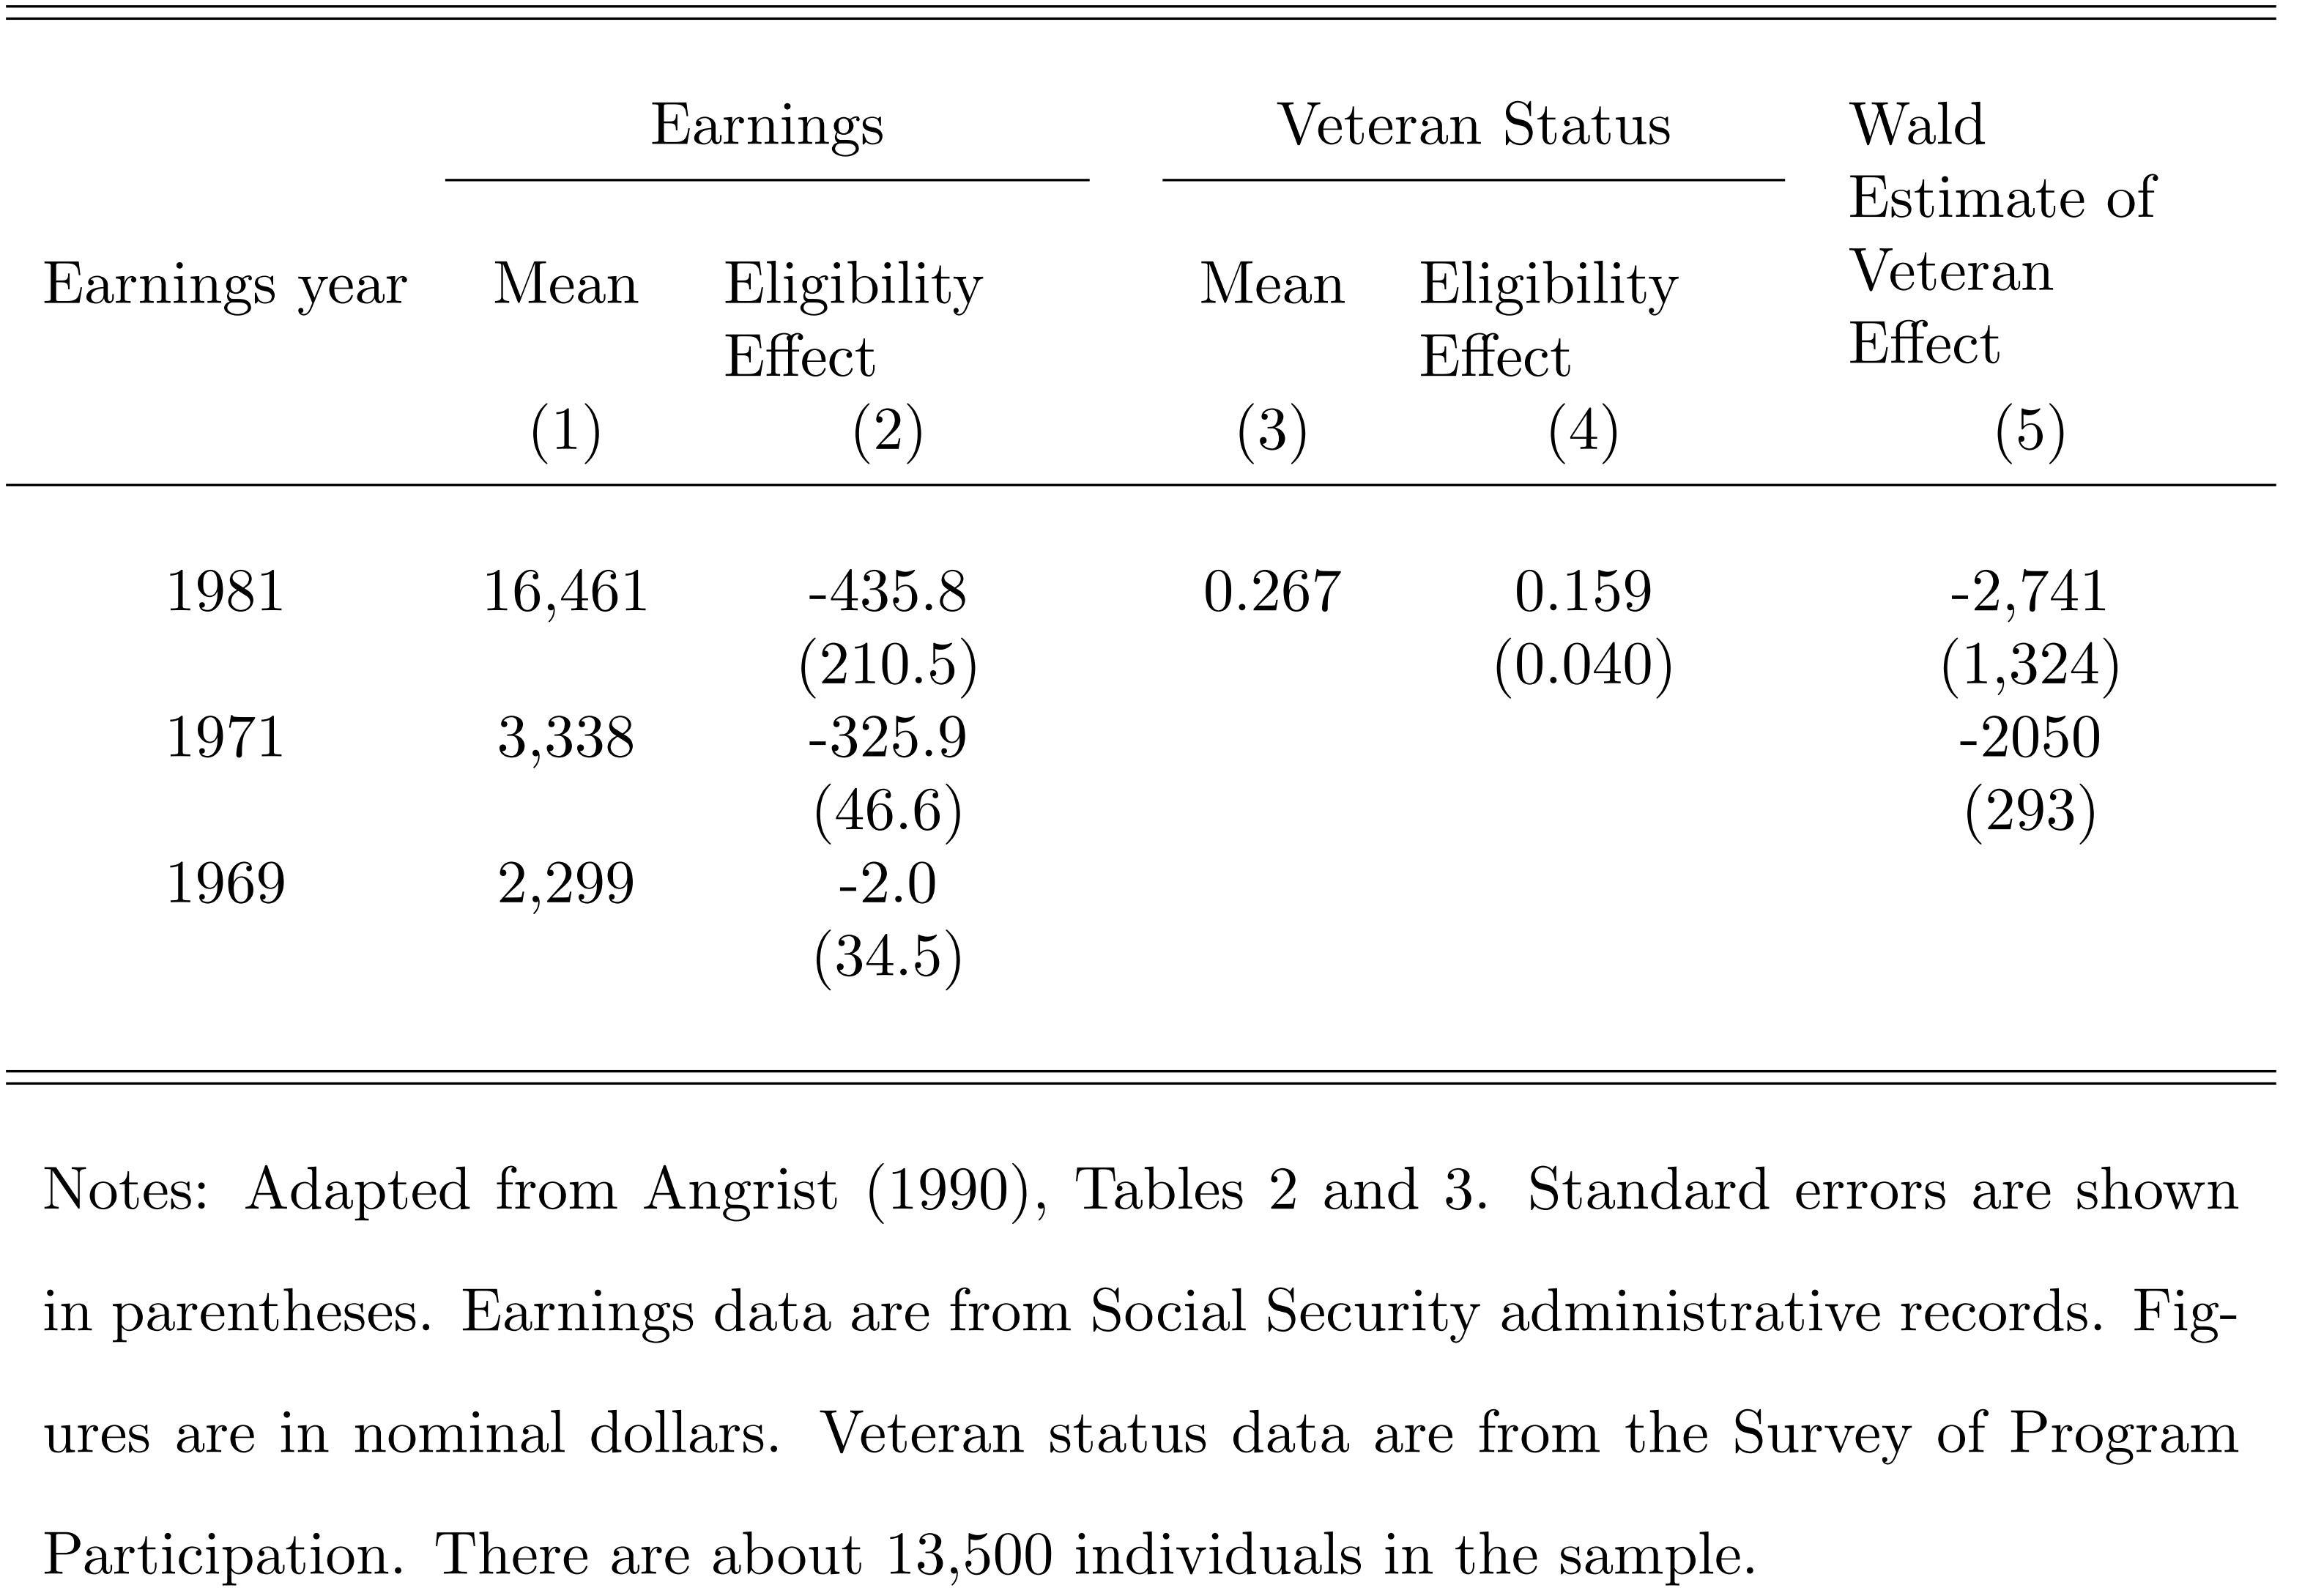
\includegraphics[width=0.9\textwidth]{figure/lottery_f1.jpg}
		\end{figure}
	\end{center}
\end{frame}








\title[]  
{STATA Example}


\author 
{}

%\institute{Institute of Economics, Academia Sinica  \\ Econ, NTU}
%\institute{Institute of Economics, Academia Sinica  \\ IMES/IDAS, NCCU}
\institute{}

%\author 
%{楊子霆 \\ 中研院經濟所}

%\institute 
%{中正大學國際經濟專題研討}




\date
{}


\begin{frame}{}
	\titlepage
\end{frame}



\begin{frame}{Acemoglu, Johnson, and Robinson (2001)}
	Acemoglu, Johnson, and Robinson (2001) ``\textbf{The Colonial Origins of Comparative Development: An Empirical Investigation}" AER
	\begin{itemize}
		\vspace{0.2cm}
		\item They want to examine the effect of institutions on  economic development
		\vspace{0.2cm}
			\begin{itemize}
		\item Do countries with better institutions achieve a greater level of income?
					\end{itemize}

			\vspace{0.2cm}
			\item \textbf{Good institutions} include:
			\begin{itemize}
				\vspace{0.2cm}
				\item Strong protection of property rights
				\item Less distortionary policies (e.g., high tax rate)
				\item Checks and balances on government power
				\item Investment-friendly policies (e.g., rule of law, contract enforcement)
			\end{itemize}
			
			
			
			
		%	\item Good institutions: more secure property rights, less distortionary policies, invest more in physical 	and human capital
			
			

		
		
	\end{itemize}
\end{frame}





\begin{frame}{Acemoglu, Johnson, and Robinson (2001)}{Motivation}
	
	\begin{center}
		\begin{figure}[p]
			\centering
			
\includegraphics[width=0.6\textwidth]{figure/nobel_2024.jpg}
		\end{figure}
	\end{center}
\end{frame}



\begin{frame}{Overview}{Program and Data}
	\begin{itemize}
		
		\item See IV.do
				\vspace{0.2cm}
				\item Use AJR\_table4.dta
		
						\vspace{0.2cm}
		\item If you want to know the complete programs and data for this paper, please use the following:
								\vspace{0.2cm}
			\begin{itemize}
		\item AJR-IV.do
		\vspace{0.2cm}
		\item Use AJR\_table2.dta to AJR\_table7.dta
			\end{itemize}
		
		
		
		
	\end{itemize}
\end{frame}



\begin{frame}{Acemoglu, Johnson, and Robinson (2001)}{Motivation}
	\begin{itemize}
		\item At some level  it is obvious that institutions 
		matter
		\vspace{0.2cm}
		\item  Witness, for  example, the  divergent paths of North and South Korea, or East and West German
		\vspace{0.2cm}
		\begin{itemize}
			\item  central planning and collective ownership V.S. private property and market economy
			
			
		\end{itemize}
		
		
		
	\end{itemize}
	
\end{frame}



\begin{frame}{Acemoglu, Johnson, and Robinson (2001)}{Motivation}
	
	\begin{center}
		\begin{figure}[p]
			\centering
			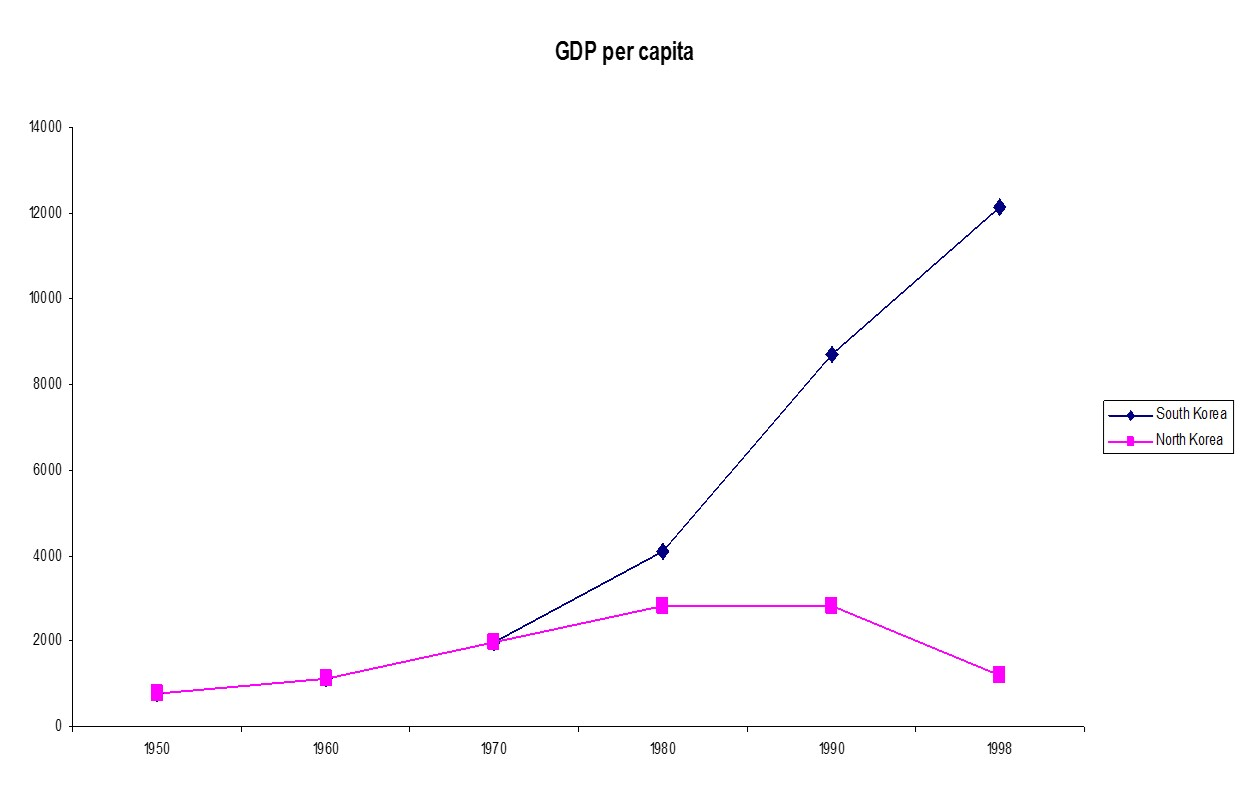
\includegraphics[width=0.9\textwidth]{figure/korea_f1.jpg}
		\end{figure}
	\end{center}
\end{frame}





\begin{frame}{Acemoglu, Johnson, and Robinson (2001)}{Motivation}
	\begin{itemize}
		\item Nevertheless, we lack  reliable  estimates  of 
		the effect  of institutions on economic performance
		\vspace{0.2cm}
			\begin{itemize}
		\item \textbf{Selection bias 1}: It is  quite likely that rich economies 
		choose or can afford better institutions
		\vspace{0.2cm}
		\item \textbf{Selection bias 2}: Economies that are different for a variety of reasons will differ both in their institutions and in  their income per capita
			\end{itemize}
		\vspace{0.2cm}
		\item Need to eliminate selection bias
		
	\end{itemize}
\end{frame}




\begin{frame}{Acemoglu, Johnson, and Robinson (2001)}{Identification Strategy}
	\begin{itemize}
		\item They propose an IV to generate an exogenous variation in institution based on theory plus history 
		\vspace{0.2cm}
		\item They look only among former European colonies
		
		
	\end{itemize}
\end{frame}




\begin{frame}{Acemoglu, Johnson, and Robinson (2001)}{Identification Strategy}
	\begin{itemize}
		\item Their theory is based on the following facts:
		\vspace{0.2cm}
			\begin{itemize}
		\item[1] In some colonies, Europeans had good survival, in others not
		\vspace{0.2cm}
		\item[2] Where Europeans could survive, they put down roots, established good institutions
		\vspace{0.2cm}
		\begin{itemize}
			\item Replicate European institutions, with strong 
			emphasis on private property and checks against government power
		\end{itemize}
			\end{itemize}
	\end{itemize}
\end{frame}






\begin{frame}{Acemoglu, Johnson, and Robinson (2001)}{Identification Strategy}
	\begin{itemize}
		\item[3] Where they were dying like flies, they set up extractive institutions
		\vspace{0.2cm}
		\item[4] Extractive institutions designed to get resources quickly
		\vspace{0.2cm}
		\begin{itemize}
			\item  Extractive institutions did not introduce much protection for private property, nor did they provide checks and balances against government expropriation
		\end{itemize}
		\vspace{0.2cm}
		\item These institutions persisted after decolonialization
		
	\end{itemize}
\end{frame}



\begin{frame}{Acemoglu, Johnson, and Robinson (2001)}{Identification Strategy}
	\begin{itemize}
		\item They use \textbf{mortality rates expected by the first European settlers} in the colonies as an IV for current institutions in these countries
		\vspace{0.2cm}
		\item  Malaria and yellow fever were the major sources of European mortality in the colonies
		\vspace{0.2cm}
		\item Their theory is:
		\vspace{0.2cm}
		\item[] Health environment $\Rightarrow$ Settler mortality $\Rightarrow$ European settlement
		$\Rightarrow$ Early institutions $\Rightarrow$ Current institutions $\Rightarrow$ Output today
		
		
		
	\end{itemize}
\end{frame}


\begin{frame}{Acemoglu, Johnson, and Robinson (2001)}{Identification Strategy}
	\begin{itemize}
		
		\item \textbf{Key assumption -- exclusion restriction}: settler mortality can NOT affect output today by any other channel
		\vspace{0.2cm}
		\item Possible threats to identification:
		\vspace{0.2cm}
		\begin{itemize}
			\item Health environment might affect output today directly
			\vspace{0.2cm}
			\item Having European settlers affects output through some channel other than institutions (language, human capital)
		\end{itemize}
		
		
		
		
	\end{itemize}
\end{frame}


\begin{frame}{Acemoglu, Johnson, and Robinson (2001)}{Identification Strategy}
	\begin{itemize}
		
		\item Yellow fever and malaria had much less effect on native inhabitants, who had acquired and genetic immunity
		\vspace{0.2cm}
			\begin{itemize}
		\item  The prevalence of these diseases depend on the microclimate  of an area (e.g. temperature and 
		humidity)
		\vspace{0.2cm}
			\end{itemize}
		\item This suggests that mortality rates faced by Europeans are unlikely to be a proxy for some simple geographic or climatic feature of the country 
		
		
	\end{itemize}
\end{frame}



\begin{frame}{Acemoglu, Johnson, and Robinson (2001)}{TSLS estimation}
	\begin{itemize}
		
		\item They conduct a TSLS estimation
		\vspace{0.2cm}
			\begin{itemize}
		\item \textbf{First stage}: current economic institutions = g(settler mortality)
		\vspace{0.2cm}
		\item \textbf{Second stage}: log income per capita = f(current economic institutions)
			\end{itemize}
	\end{itemize}
\end{frame}








\begin{frame}{Acemoglu, Johnson, and Robinson (2001)}{Data}
	\begin{itemize}
		\item Mortality rates of soldiers stationed in the colonies in the early 19th century
		\vspace{0.2cm} 
		\begin{itemize}
			\item They got it from historian Philip Curtin
		\end{itemize}
		\vspace{0.2cm}
		\item \textbf{Current economic institutions} proxied by \textbf{protection against expropriation risk}
		\vspace{0.2cm}
		\begin{itemize}
			\item Average \textbf{protection against expropriation risk} is measured on a scale from 0 to 10
			\vspace{0.2cm}
			\item A higher score means more protection against 
			expropriation, averaged over 1985 to 1995, from Political Risk Services
			
			
			%\item Protection against expropriation risk proxying for many other sources of institutional variation
		\end{itemize}
		
		
		
	\end{itemize}
\end{frame}






\begin{frame}{Acemoglu, Johnson, and Robinson (2001)}{Reduced-form relationship}
	\begin{itemize}
		\item Income and Settler Mortality
	\end{itemize}
	\begin{center}
		\begin{figure}[p]
			\centering
			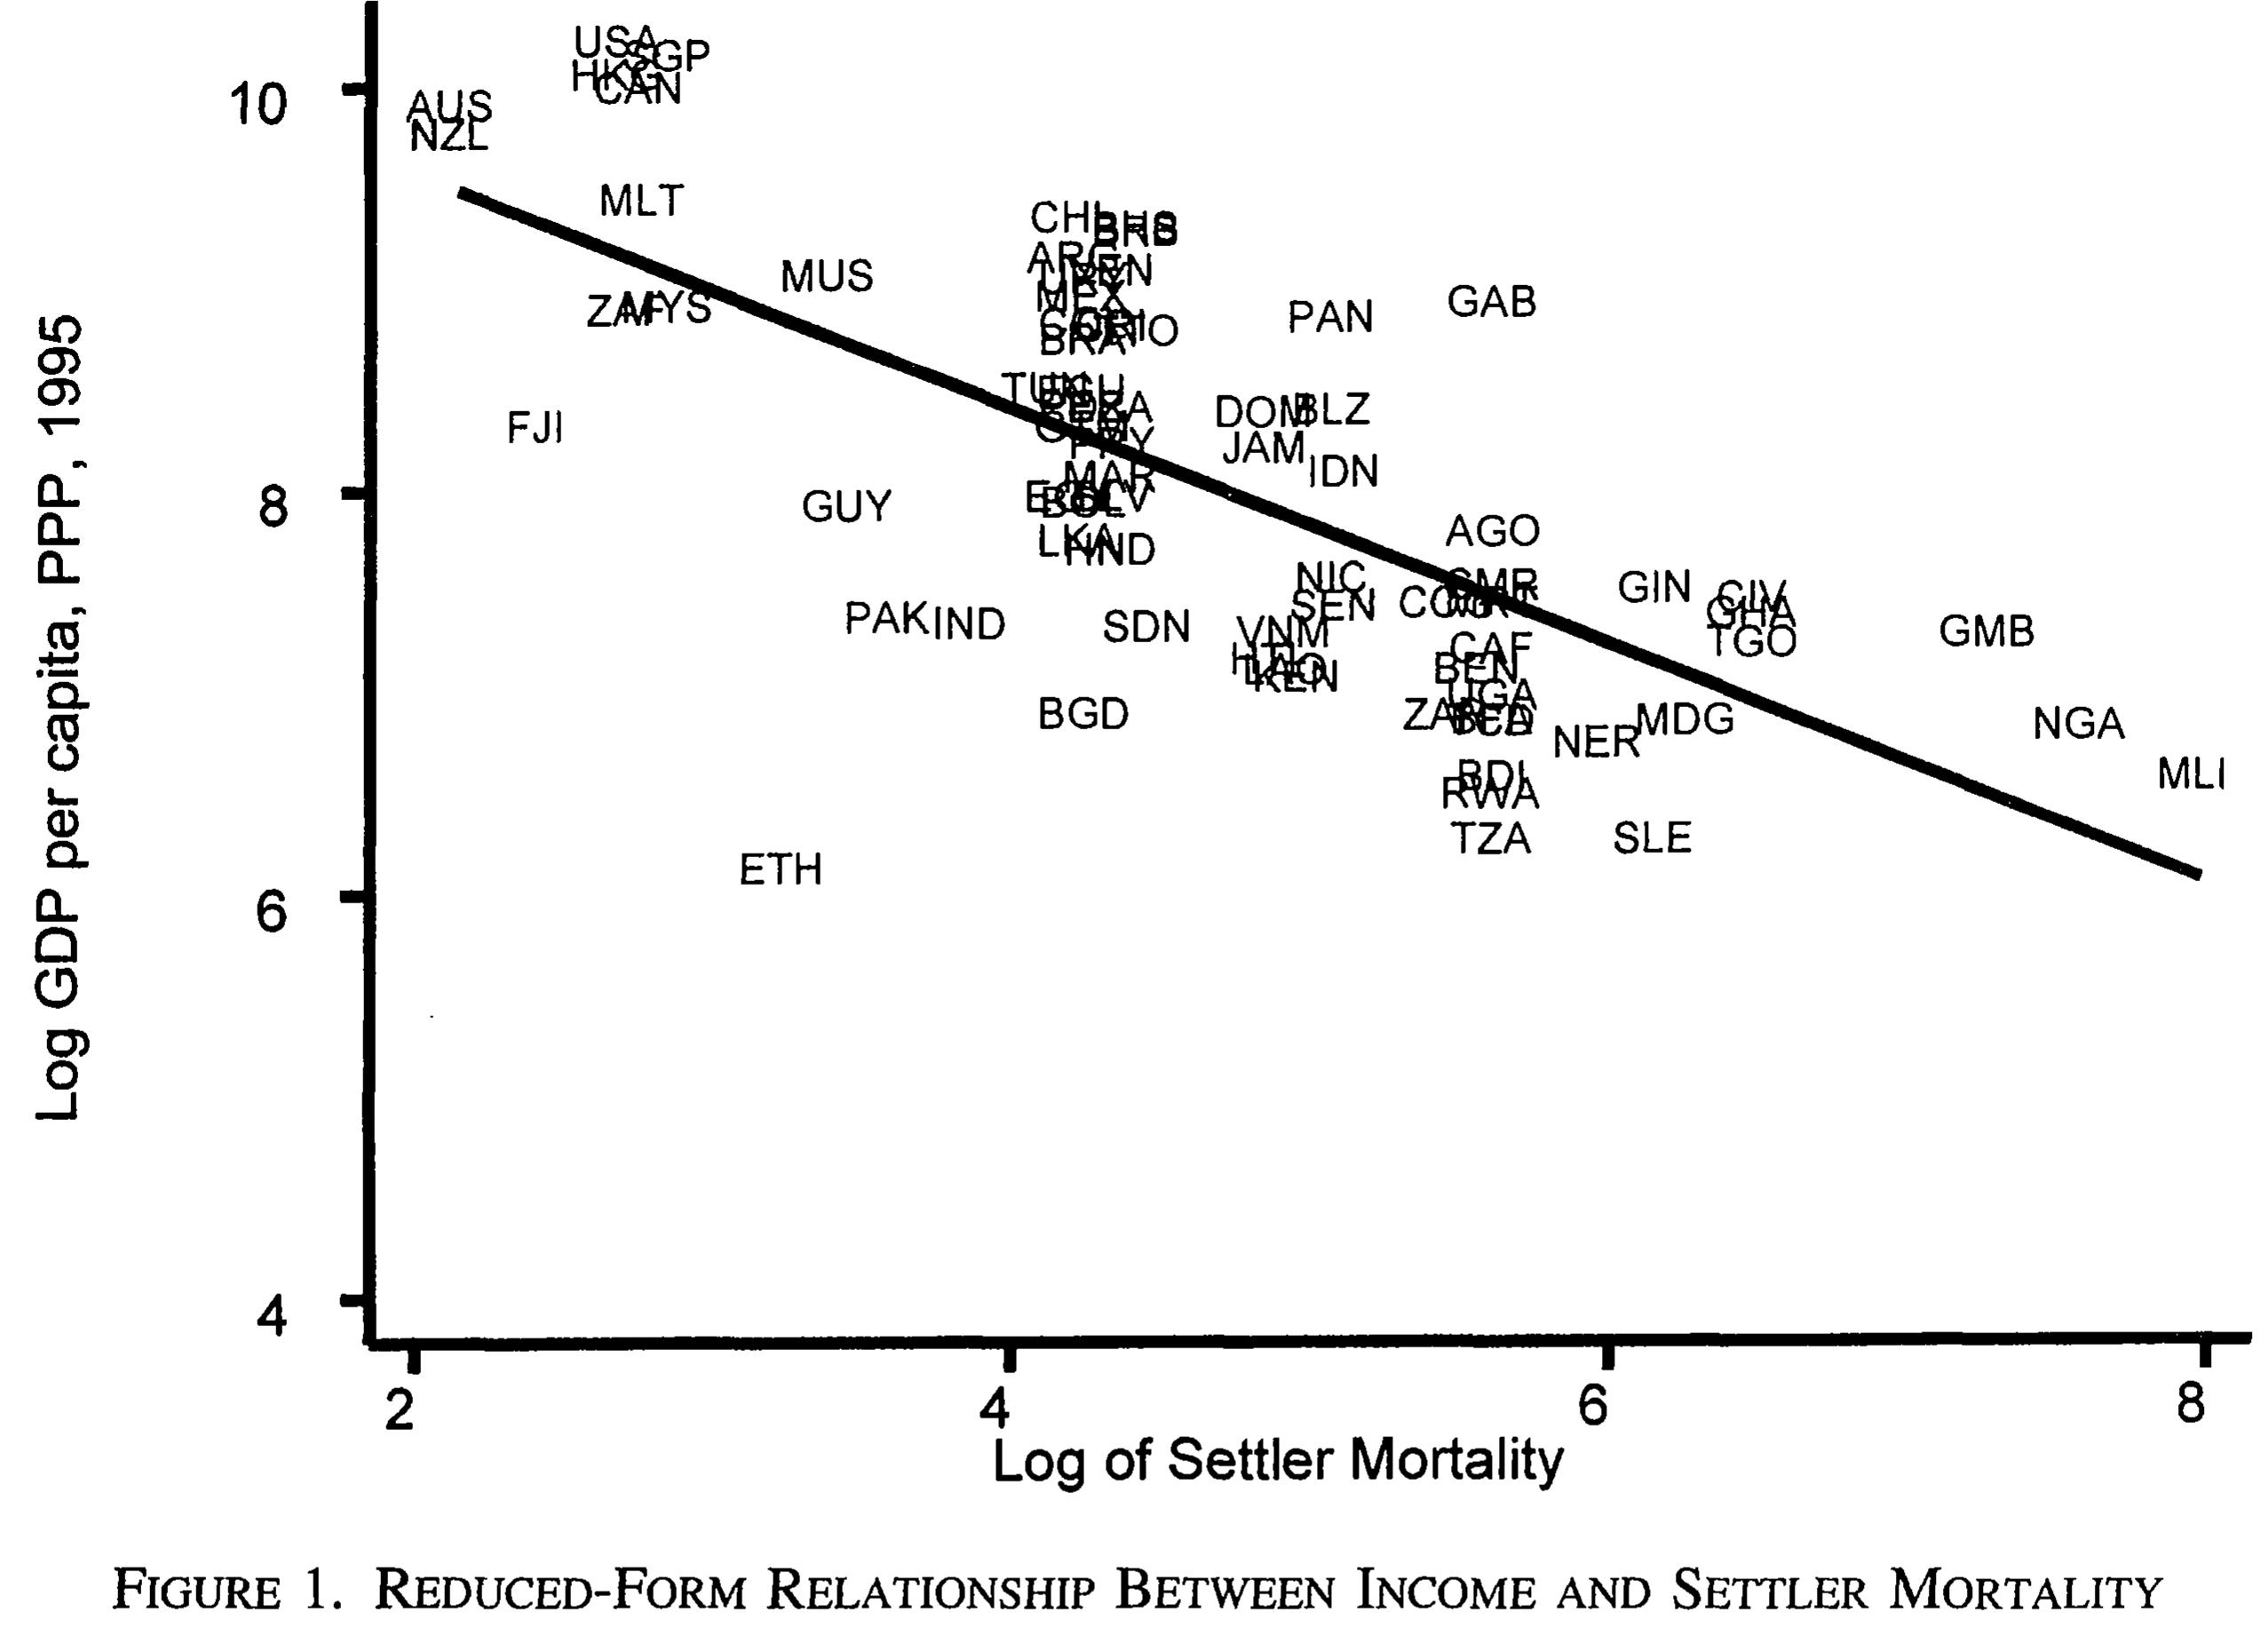
\includegraphics[width=0.7\textwidth]{figure/AJR_f1.jpg}
		\end{figure}
	\end{center}
\end{frame}



\begin{frame}{Acemoglu, Johnson, and Robinson (2001)}{First-stage relationship}
	\begin{itemize}
		\item Protection for Expropriation Risk and Settler Mortality
	\end{itemize}
	\begin{center}
		\begin{figure}[p]
			\centering
			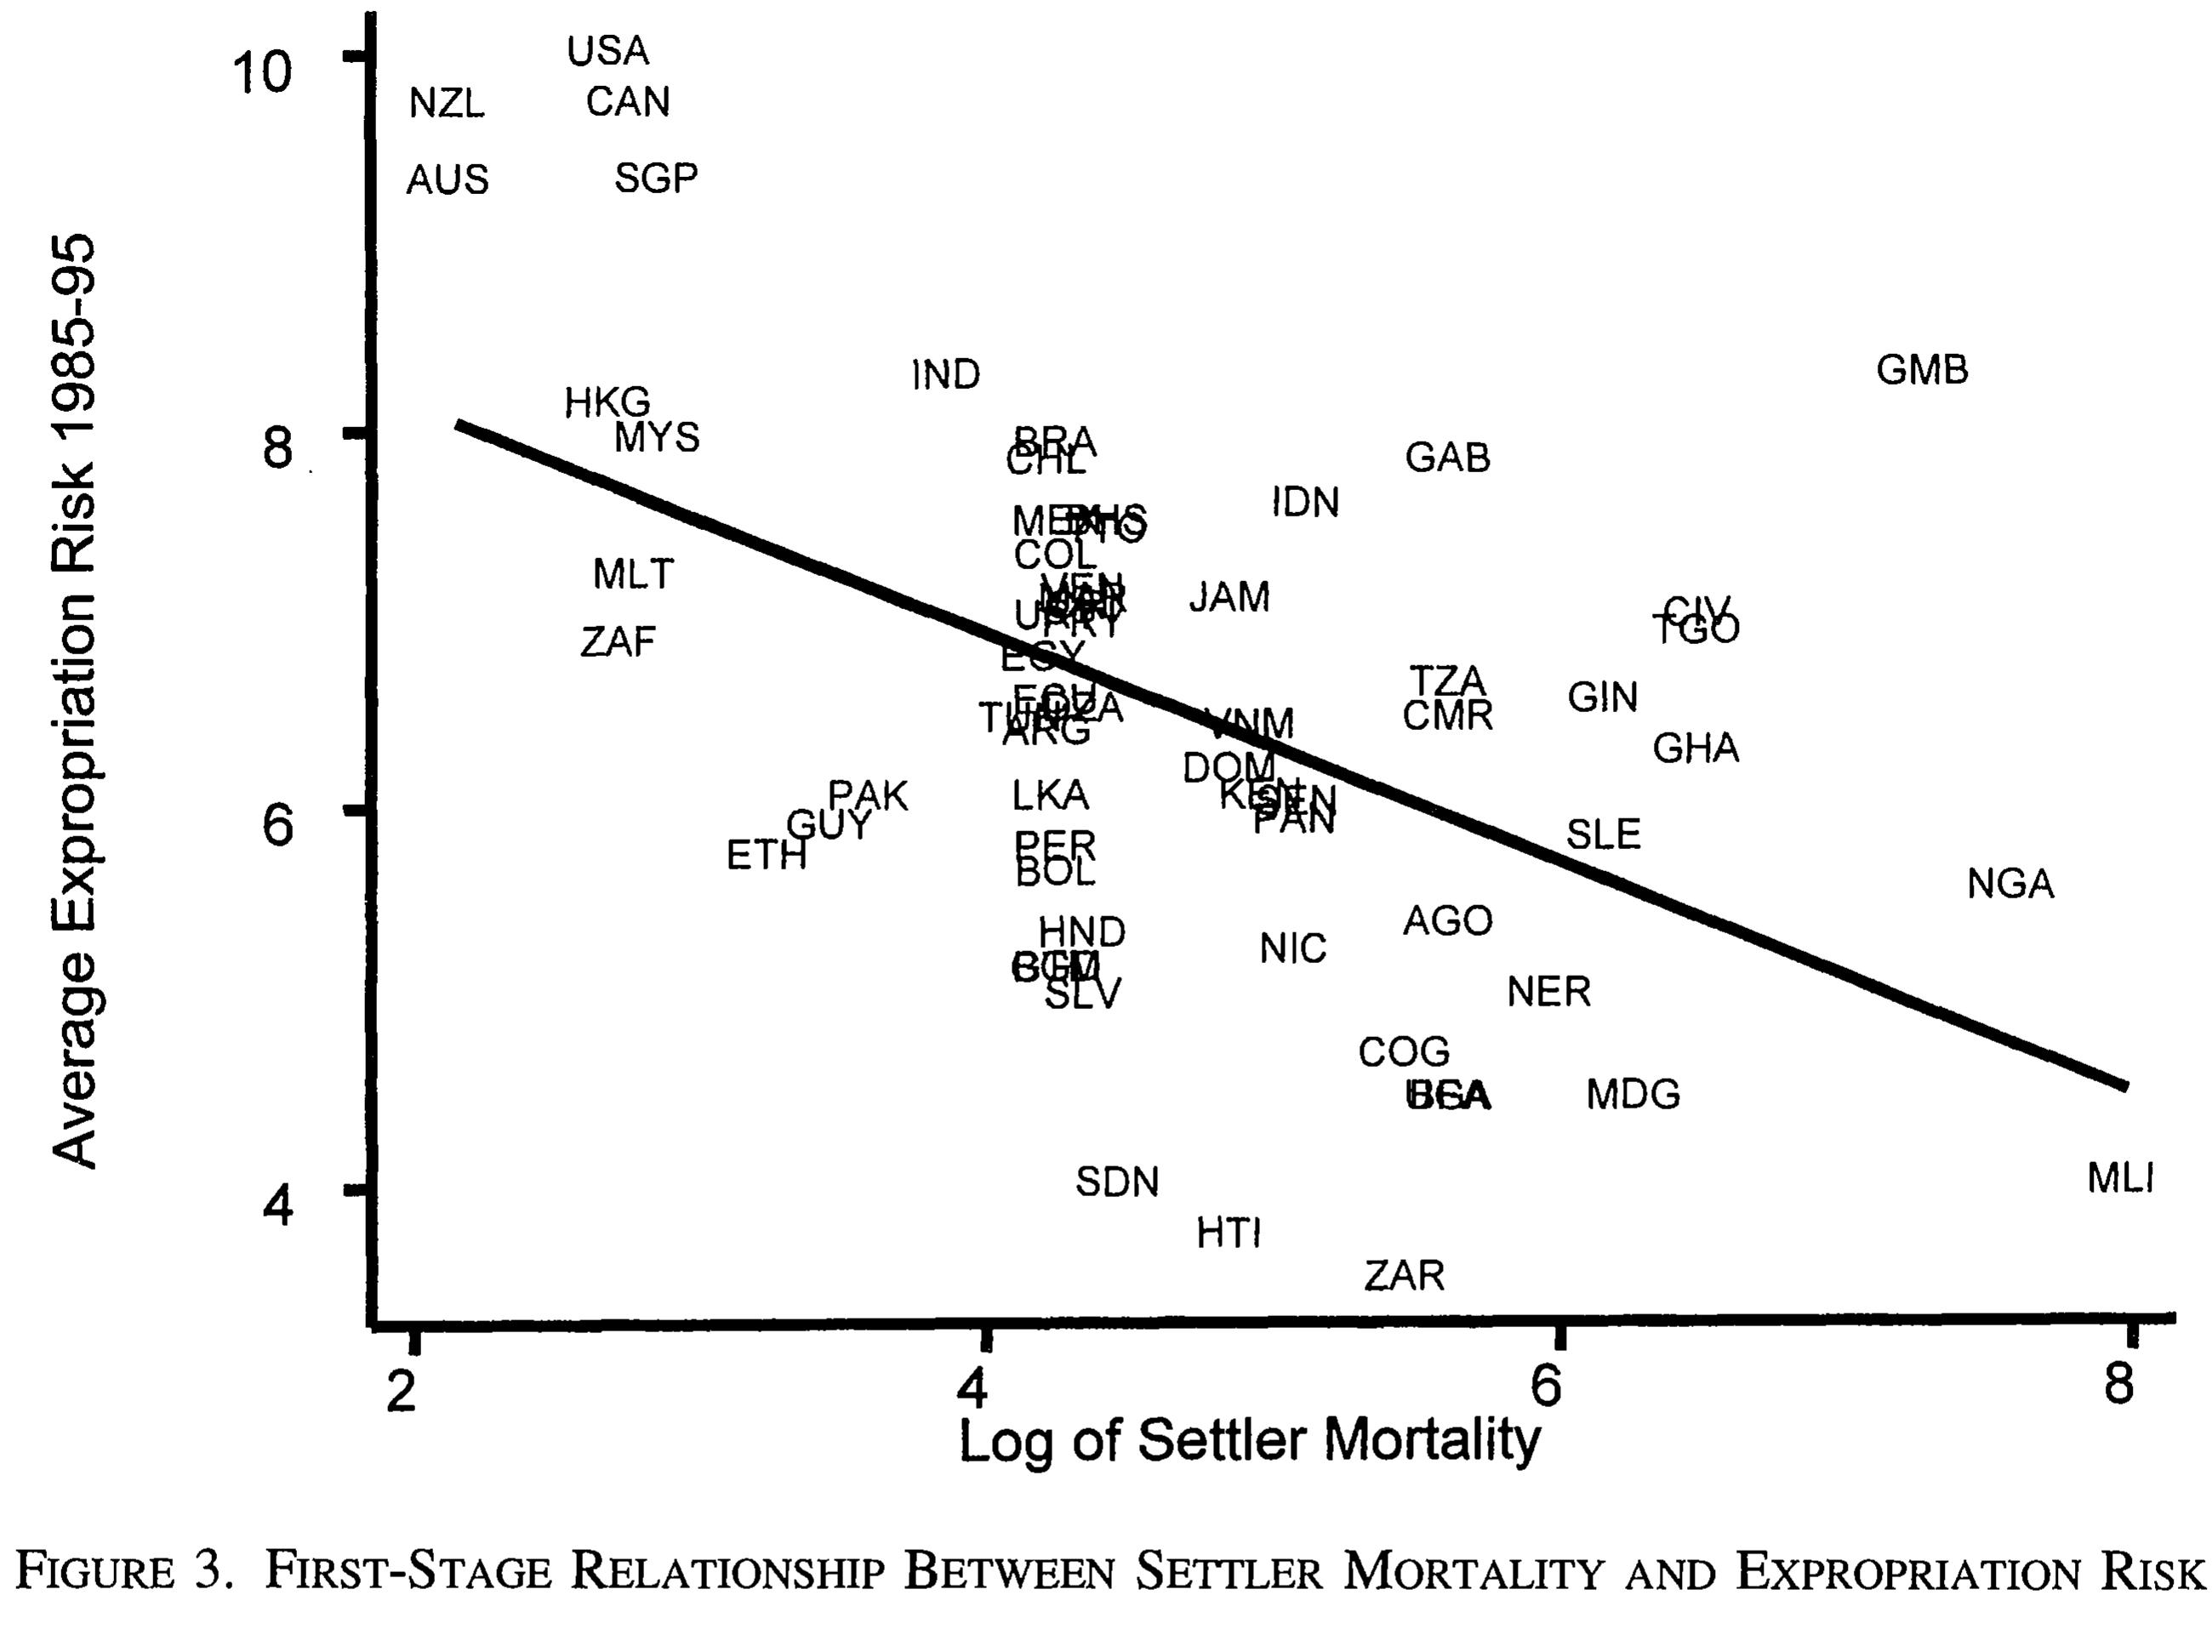
\includegraphics[width=0.7\textwidth]{figure/AJR_f3.jpg}
		\end{figure}
	\end{center}
\end{frame}



\begin{frame}{Acemoglu, Johnson, and Robinson (2001)}{Second-stage relationship}
	\begin{itemize}
		\item Protection for Expropriation Risk and Income
	\end{itemize}
	\begin{center}
		\begin{figure}[p]
			\centering
			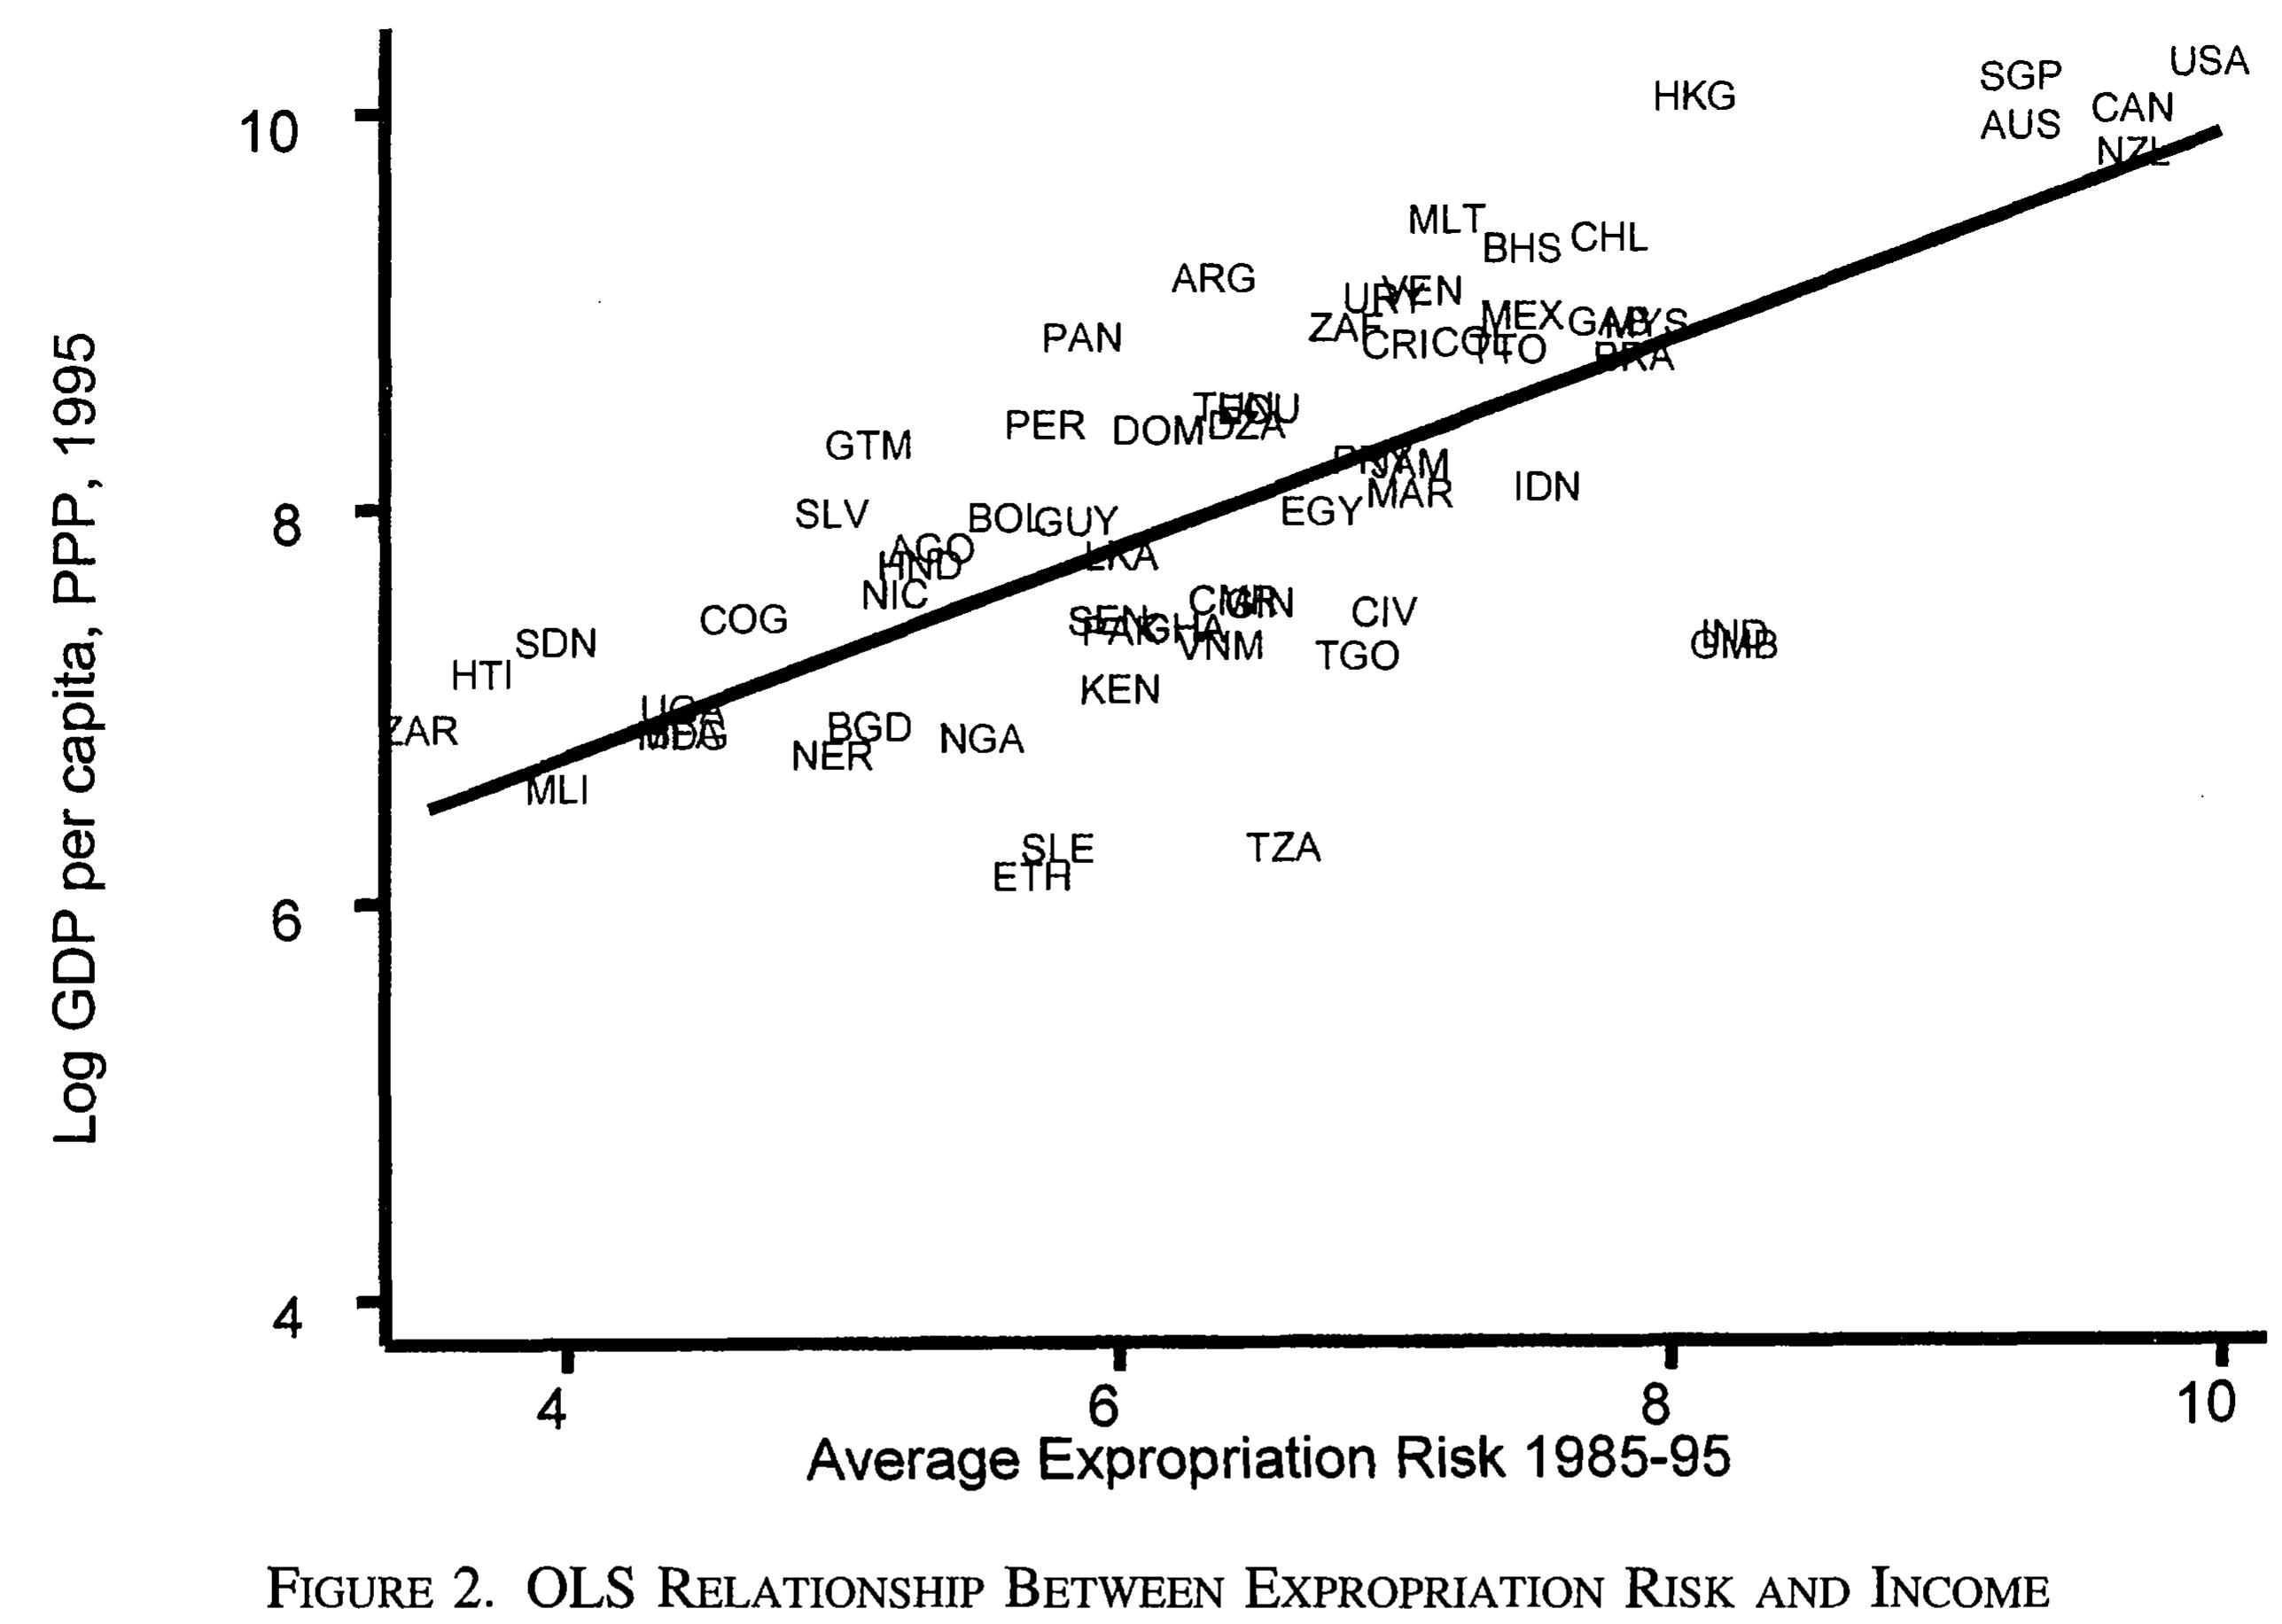
\includegraphics[width=0.7\textwidth]{figure/AJR_f2.jpg}
		\end{figure}
	\end{center}
\end{frame}





\begin{frame}{Acemoglu, Johnson, and Robinson (2001)}{Descriptive Statistics}
	
	\begin{center}
		\begin{figure}[p]
			\centering
			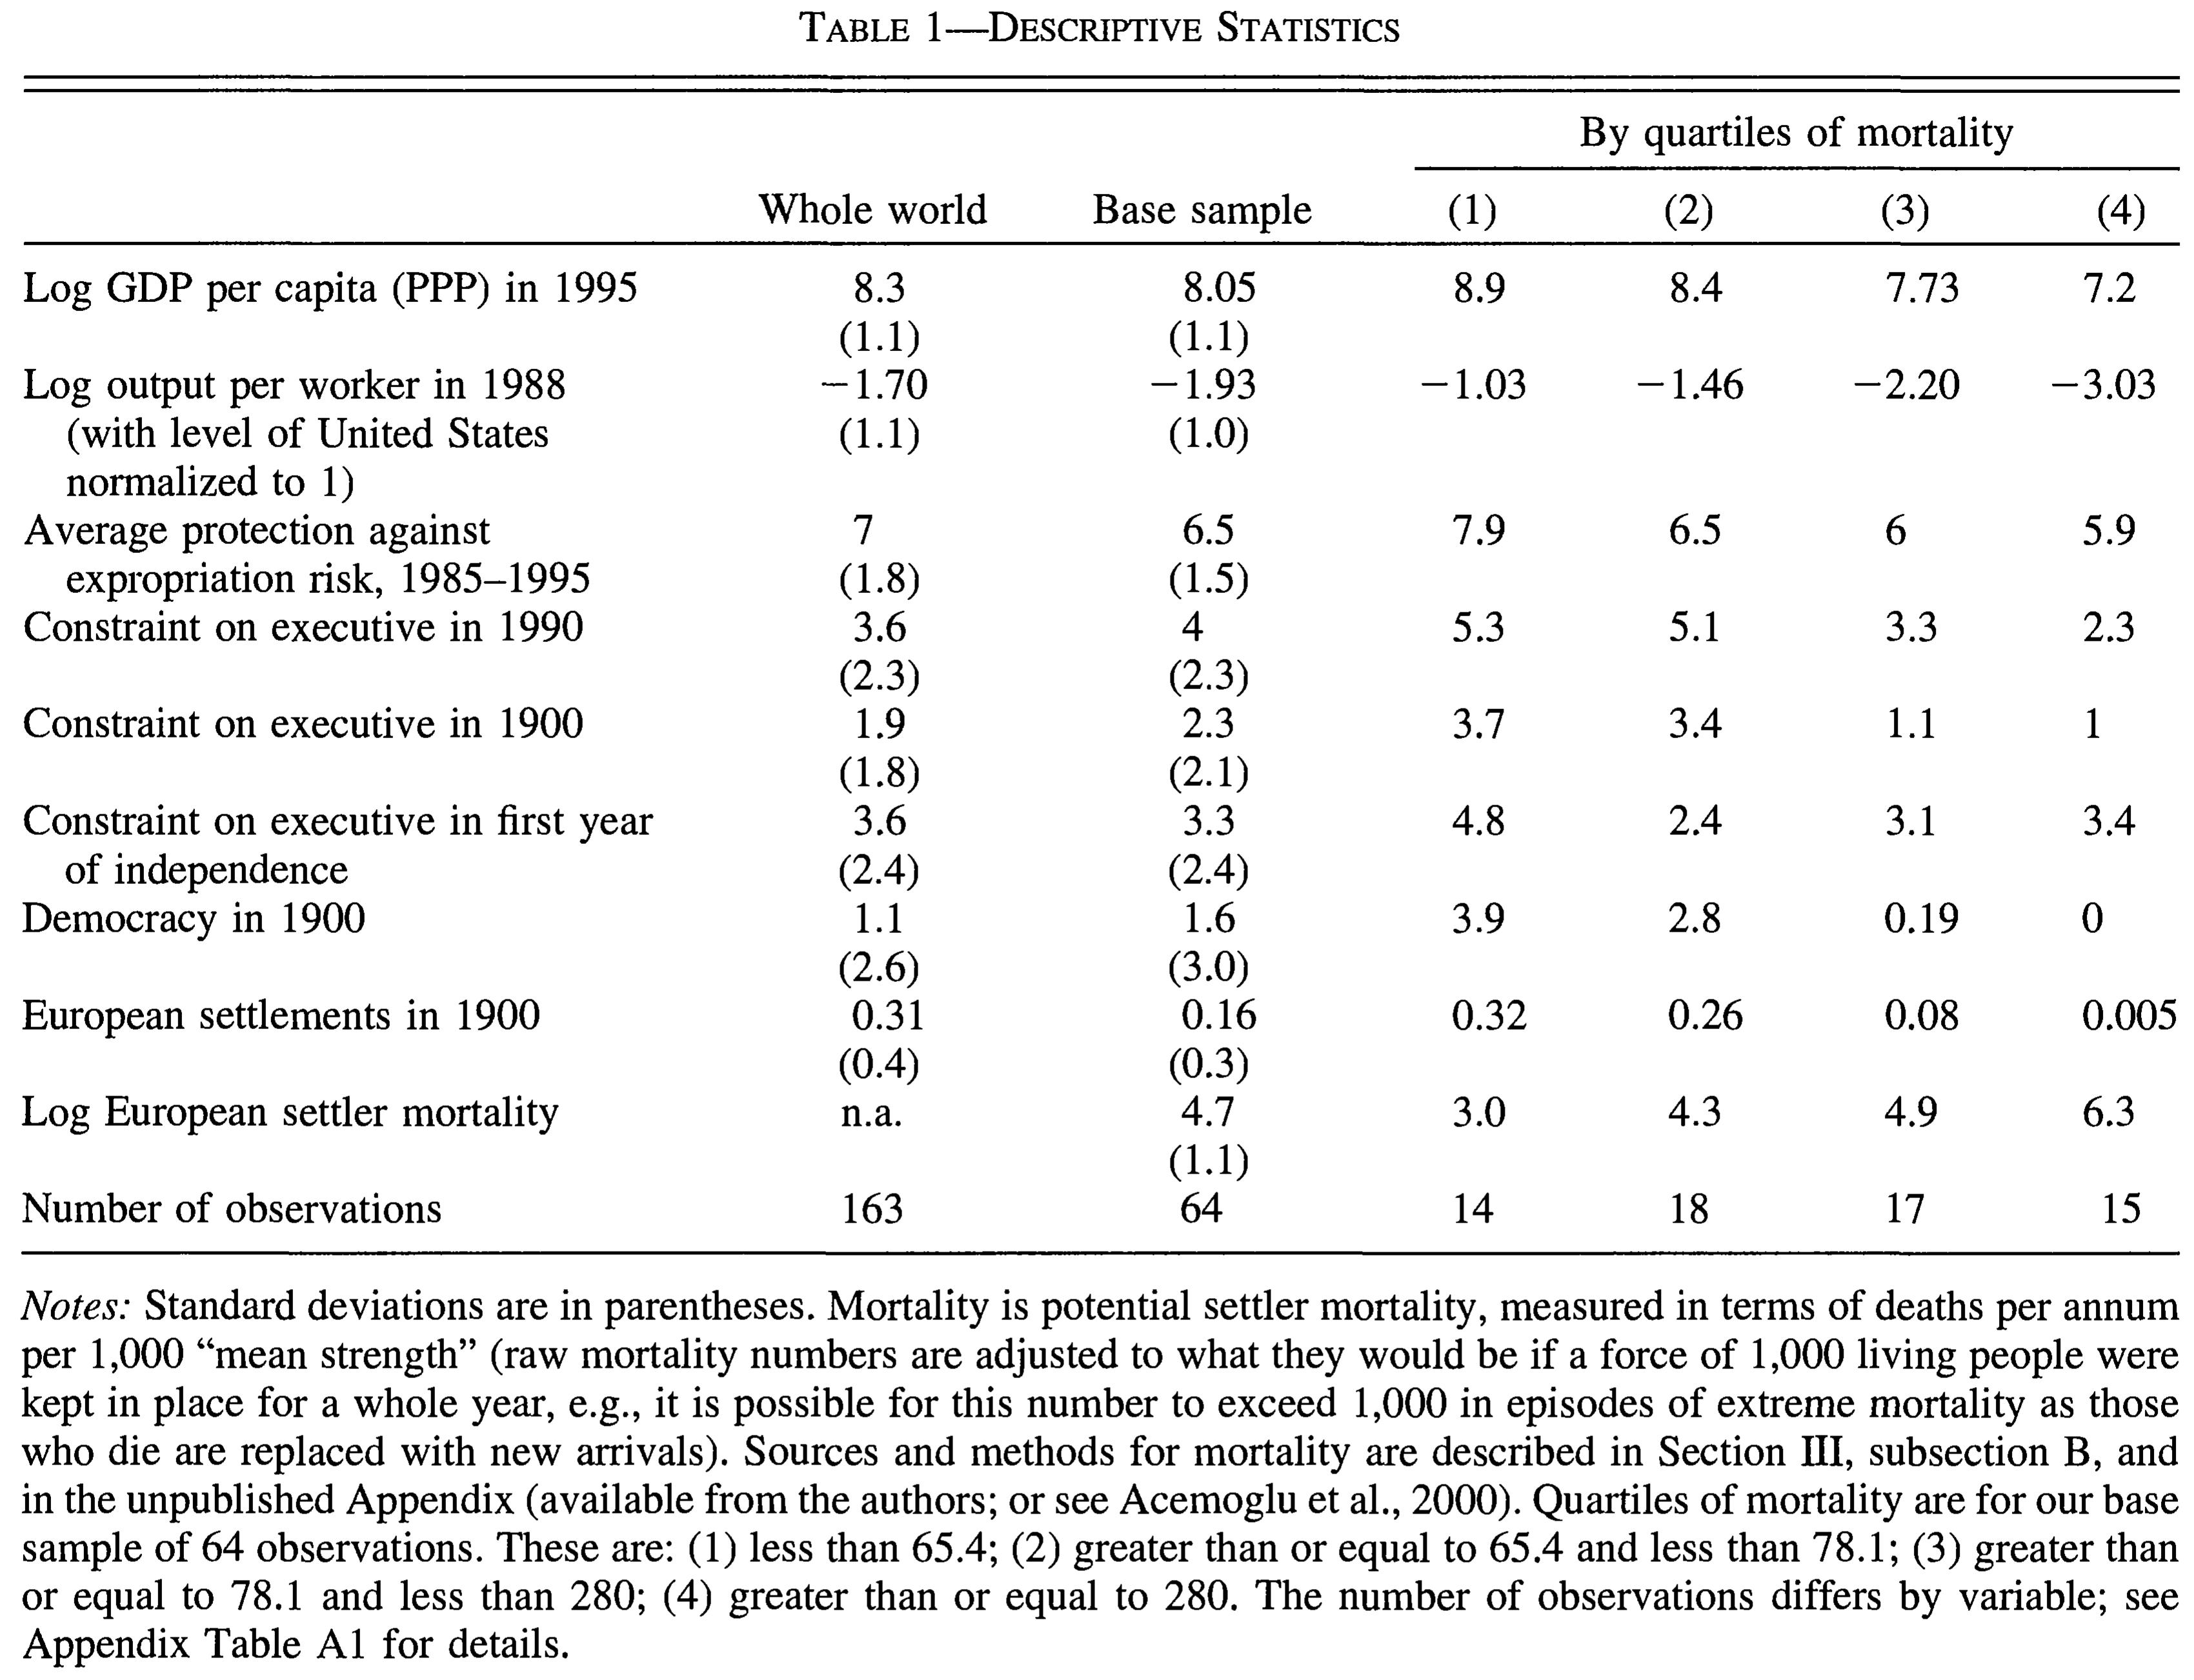
\includegraphics[width=0.8\textwidth]{figure/AJR_t1.jpg}
		\end{figure}
	\end{center}
\end{frame}





\begin{frame}{Acemoglu, Johnson, and Robinson (2001)}{OLS Results}
	
	\begin{equation*}
	log(Y_{i})= \mu +  \alpha R_i + X'_{i}\gamma + \varepsilon_{i}
	\end{equation*}
	
	\begin{itemize}
		
		\item $Y_{i}$ is income per capita in country $i$
		\vspace{0.2cm}
		\item $R_i$ is the protection against expropriation measure
		\vspace{0.2cm}
		\item $X'_{i}$ is a vector of other covariates
		\vspace{0.2cm}
		\item $\alpha$ represents the \textbf{effect of institutions on income per capita}
		
	\end{itemize}
\end{frame}



\begin{frame}{OLS Results}{STATA Implementation}

	\begin{center}
		\begin{figure}[p]
			\centering
			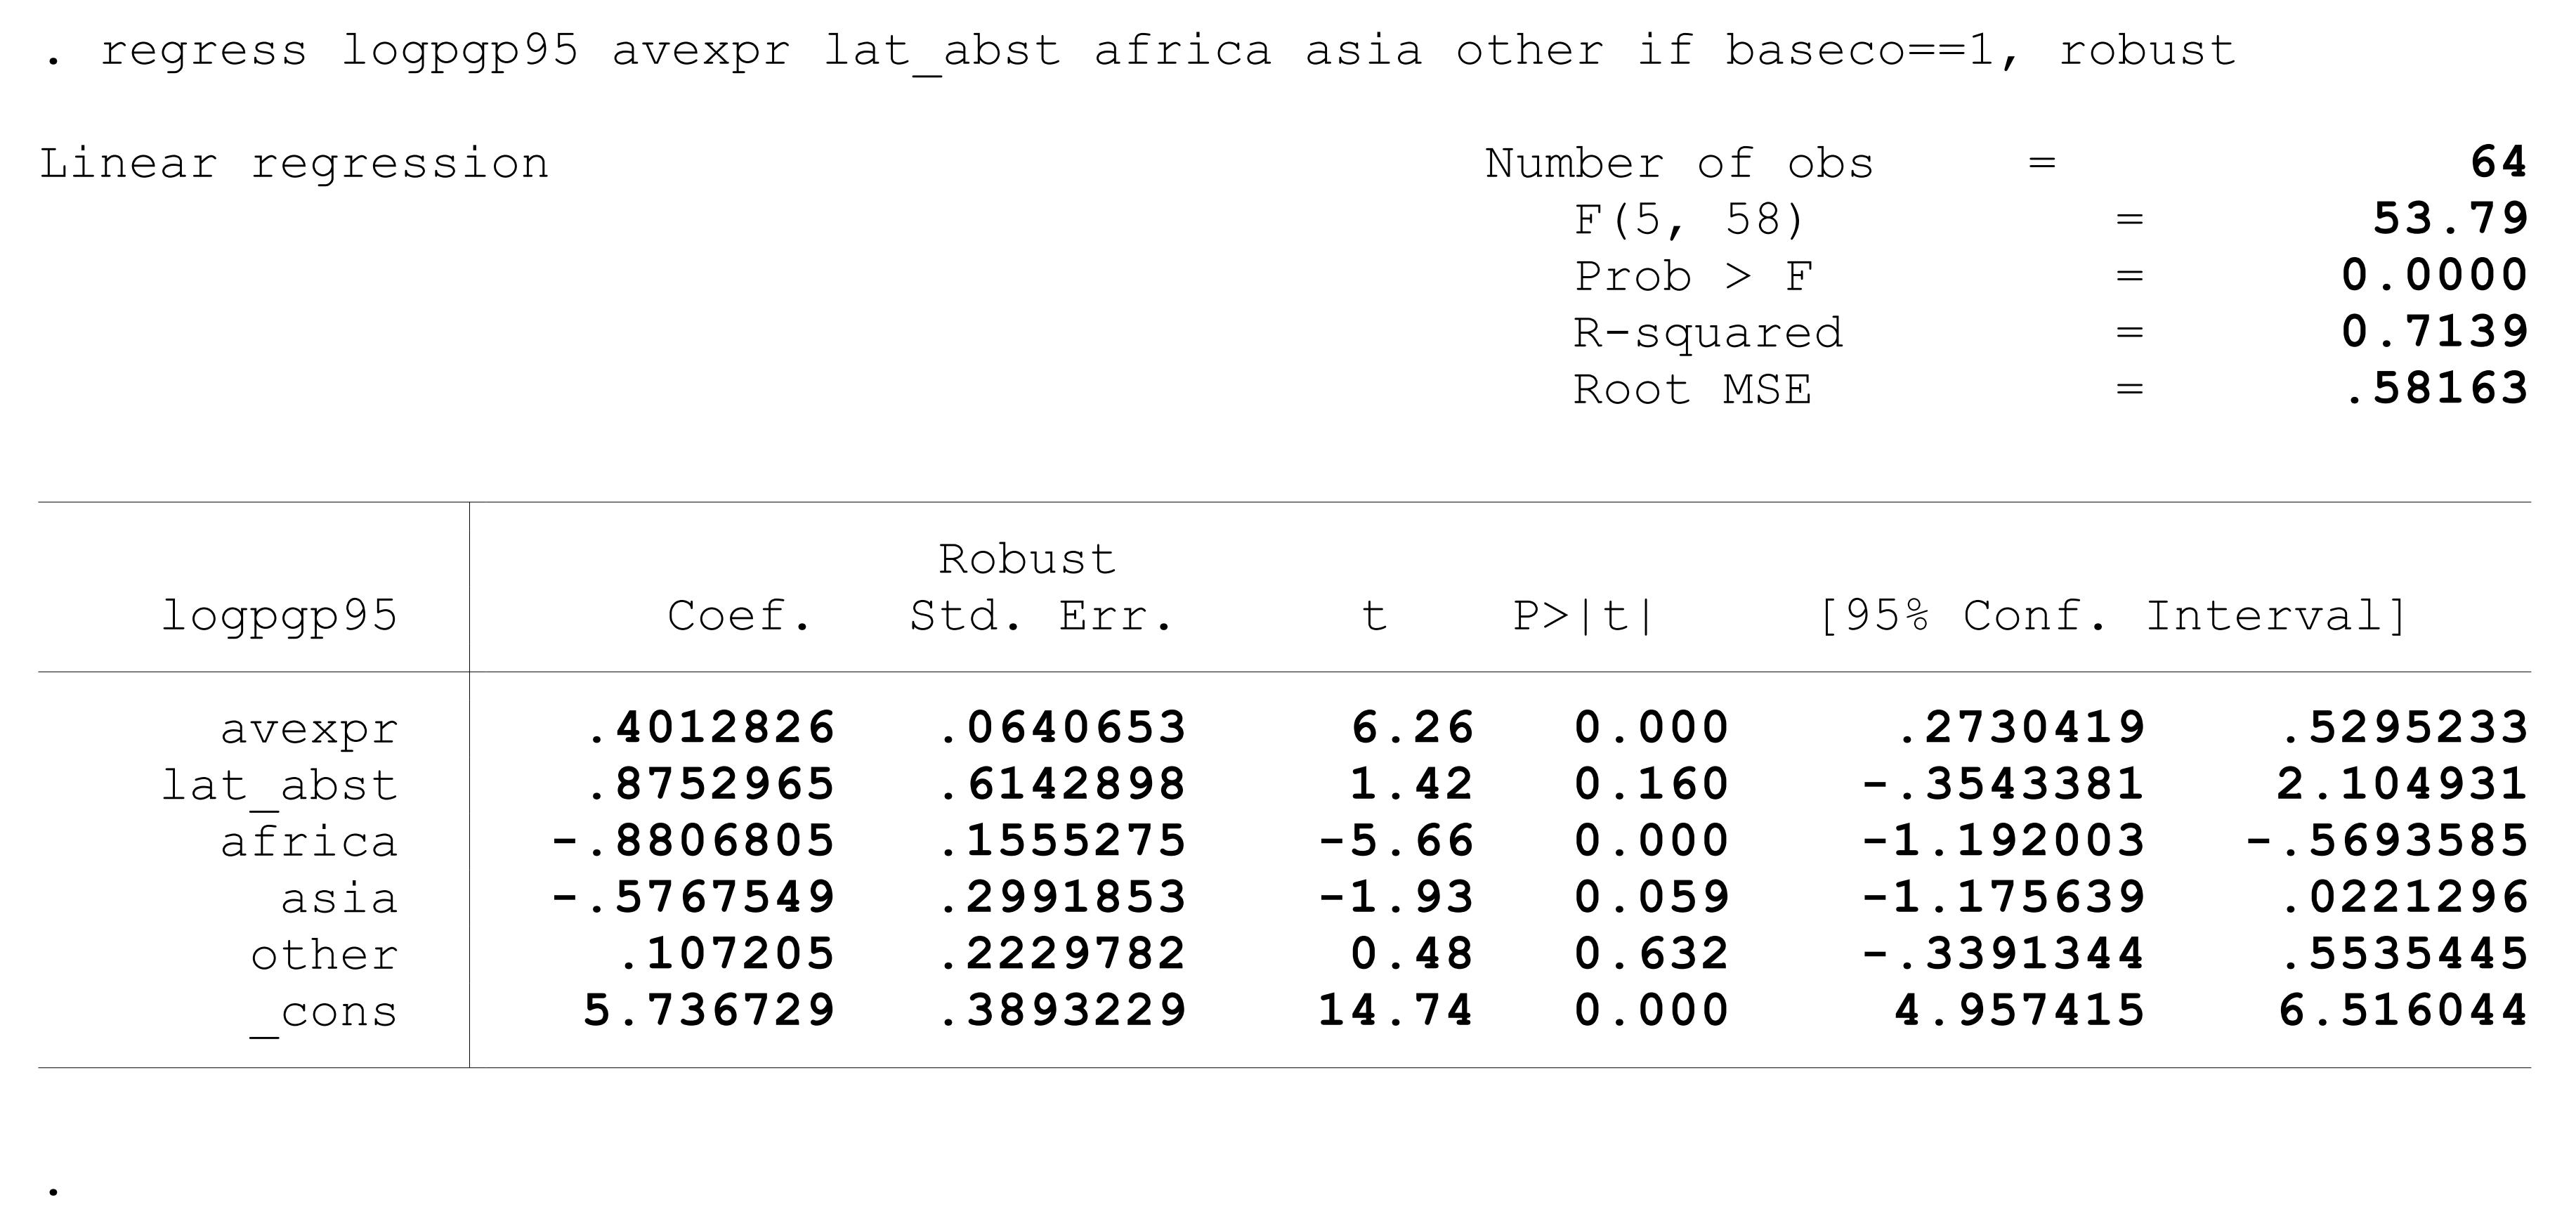
\includegraphics[width=1.0\textwidth]{figure/AJR_sta_t2_c6.jpg}
		\end{figure}
	\end{center}
\end{frame}



\begin{frame}{OLS Results}
	
	\begin{center}
		\begin{figure}[p]
			\centering
			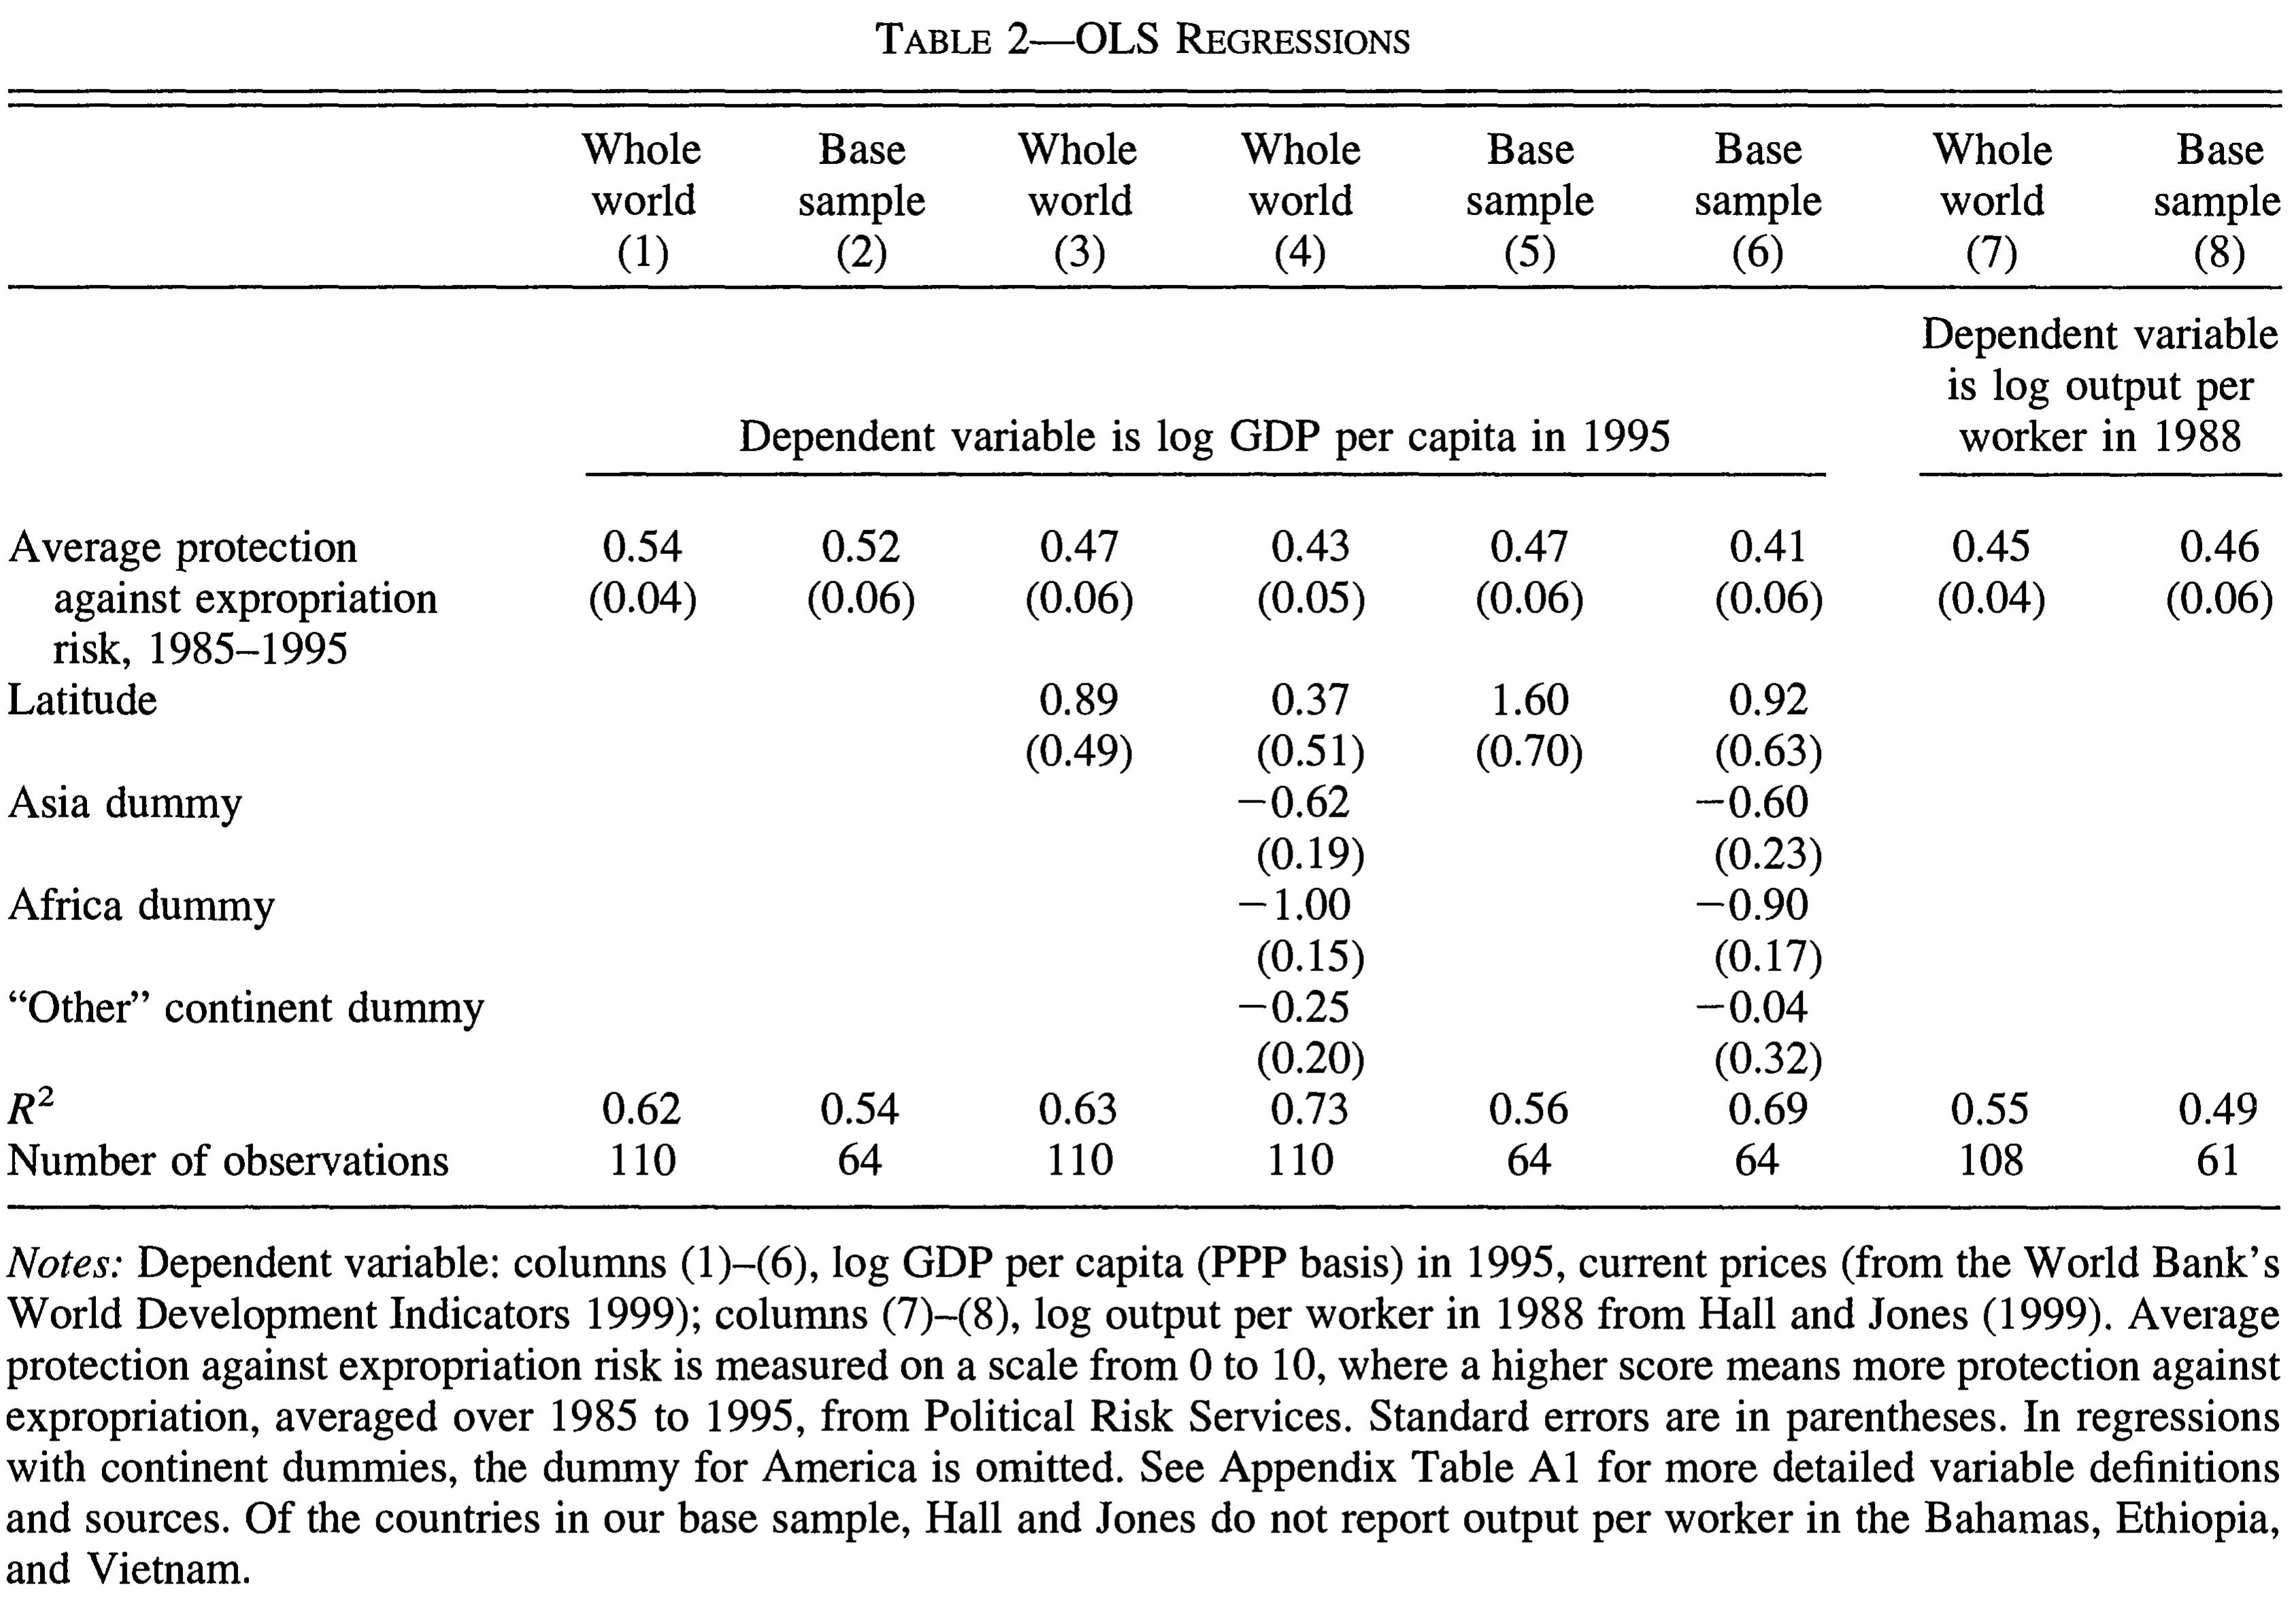
\includegraphics[width=0.9\textwidth]{figure/AJR_t2.jpg}
		\end{figure}
	\end{center}
\end{frame}



\begin{frame}{Acemoglu, Johnson, and Robinson (2001)}{IV Results}
	\begin{itemize}
		\item First stage
		\begin{equation*}
		R_{i}= \mu +  \alpha log(M_i) + X'_{i}\vartheta + \eta_{i}
		\end{equation*}
		
		\item Second stage
		\begin{equation*}
		log(Y_{i})= \mu +  \alpha R_i + X'_{i}\gamma + \varepsilon_{i}
		\end{equation*}
		
		
	\end{itemize}
	
	
	\begin{itemize}
		
		\item $M_i$ is mortality rates faced by settler at country $i$
		
		
	\end{itemize}
\end{frame}













\begin{frame}[fragile]{STATA Command: ivregress}
	\begin{itemize}
\item Syntax:
\begin{lstlisting}
ivregress estimator depvar [varlist1] (varlist2 = varlistiv) [if] [in] [weight] [, options]
\end{lstlisting}
		
\item Example:
\begin{lstlisting}
ivregress 2sls logpgp95 lat_abst africa asia other_cont (avexpr=logem4), first
estat firststage
\end{lstlisting}
		
		\vspace{0.2cm}
		\item  \textbf{varlist1}is the list of exogenous variables.
		\vspace{0.2cm}
		\item \textbf{varlist2} is the list of endogenous variables.
		\vspace{0.2cm}
		\item \textbf{varlistiv} is the list of exogenous variables used with varlist1 as instruments for varlist2.
		\vspace{0.2cm}
		\item \textbf{2sls}: two-stage least squares
	\end{itemize}
\end{frame}



\begin{frame}[fragile]{STATA Command: ivregress}
	\begin{itemize}
		\item options:
		\begin{itemize}
			\vspace{0.2cm}
			\item \textbf{estat firststage}: report first-stage F-statistic
			\vspace{0.2cm}
			\item  \textbf{level(#)}: set confidence level; default is level(95)
			\vspace{0.2cm}
			\item \textbf{first}: requests that the first-stage regression results be displayed
			
		\end{itemize}
	\end{itemize}
\end{frame}



\begin{frame}{IV Results}{STATA Implementation}
	
	\begin{center}
		\begin{figure}[p]
			\centering
			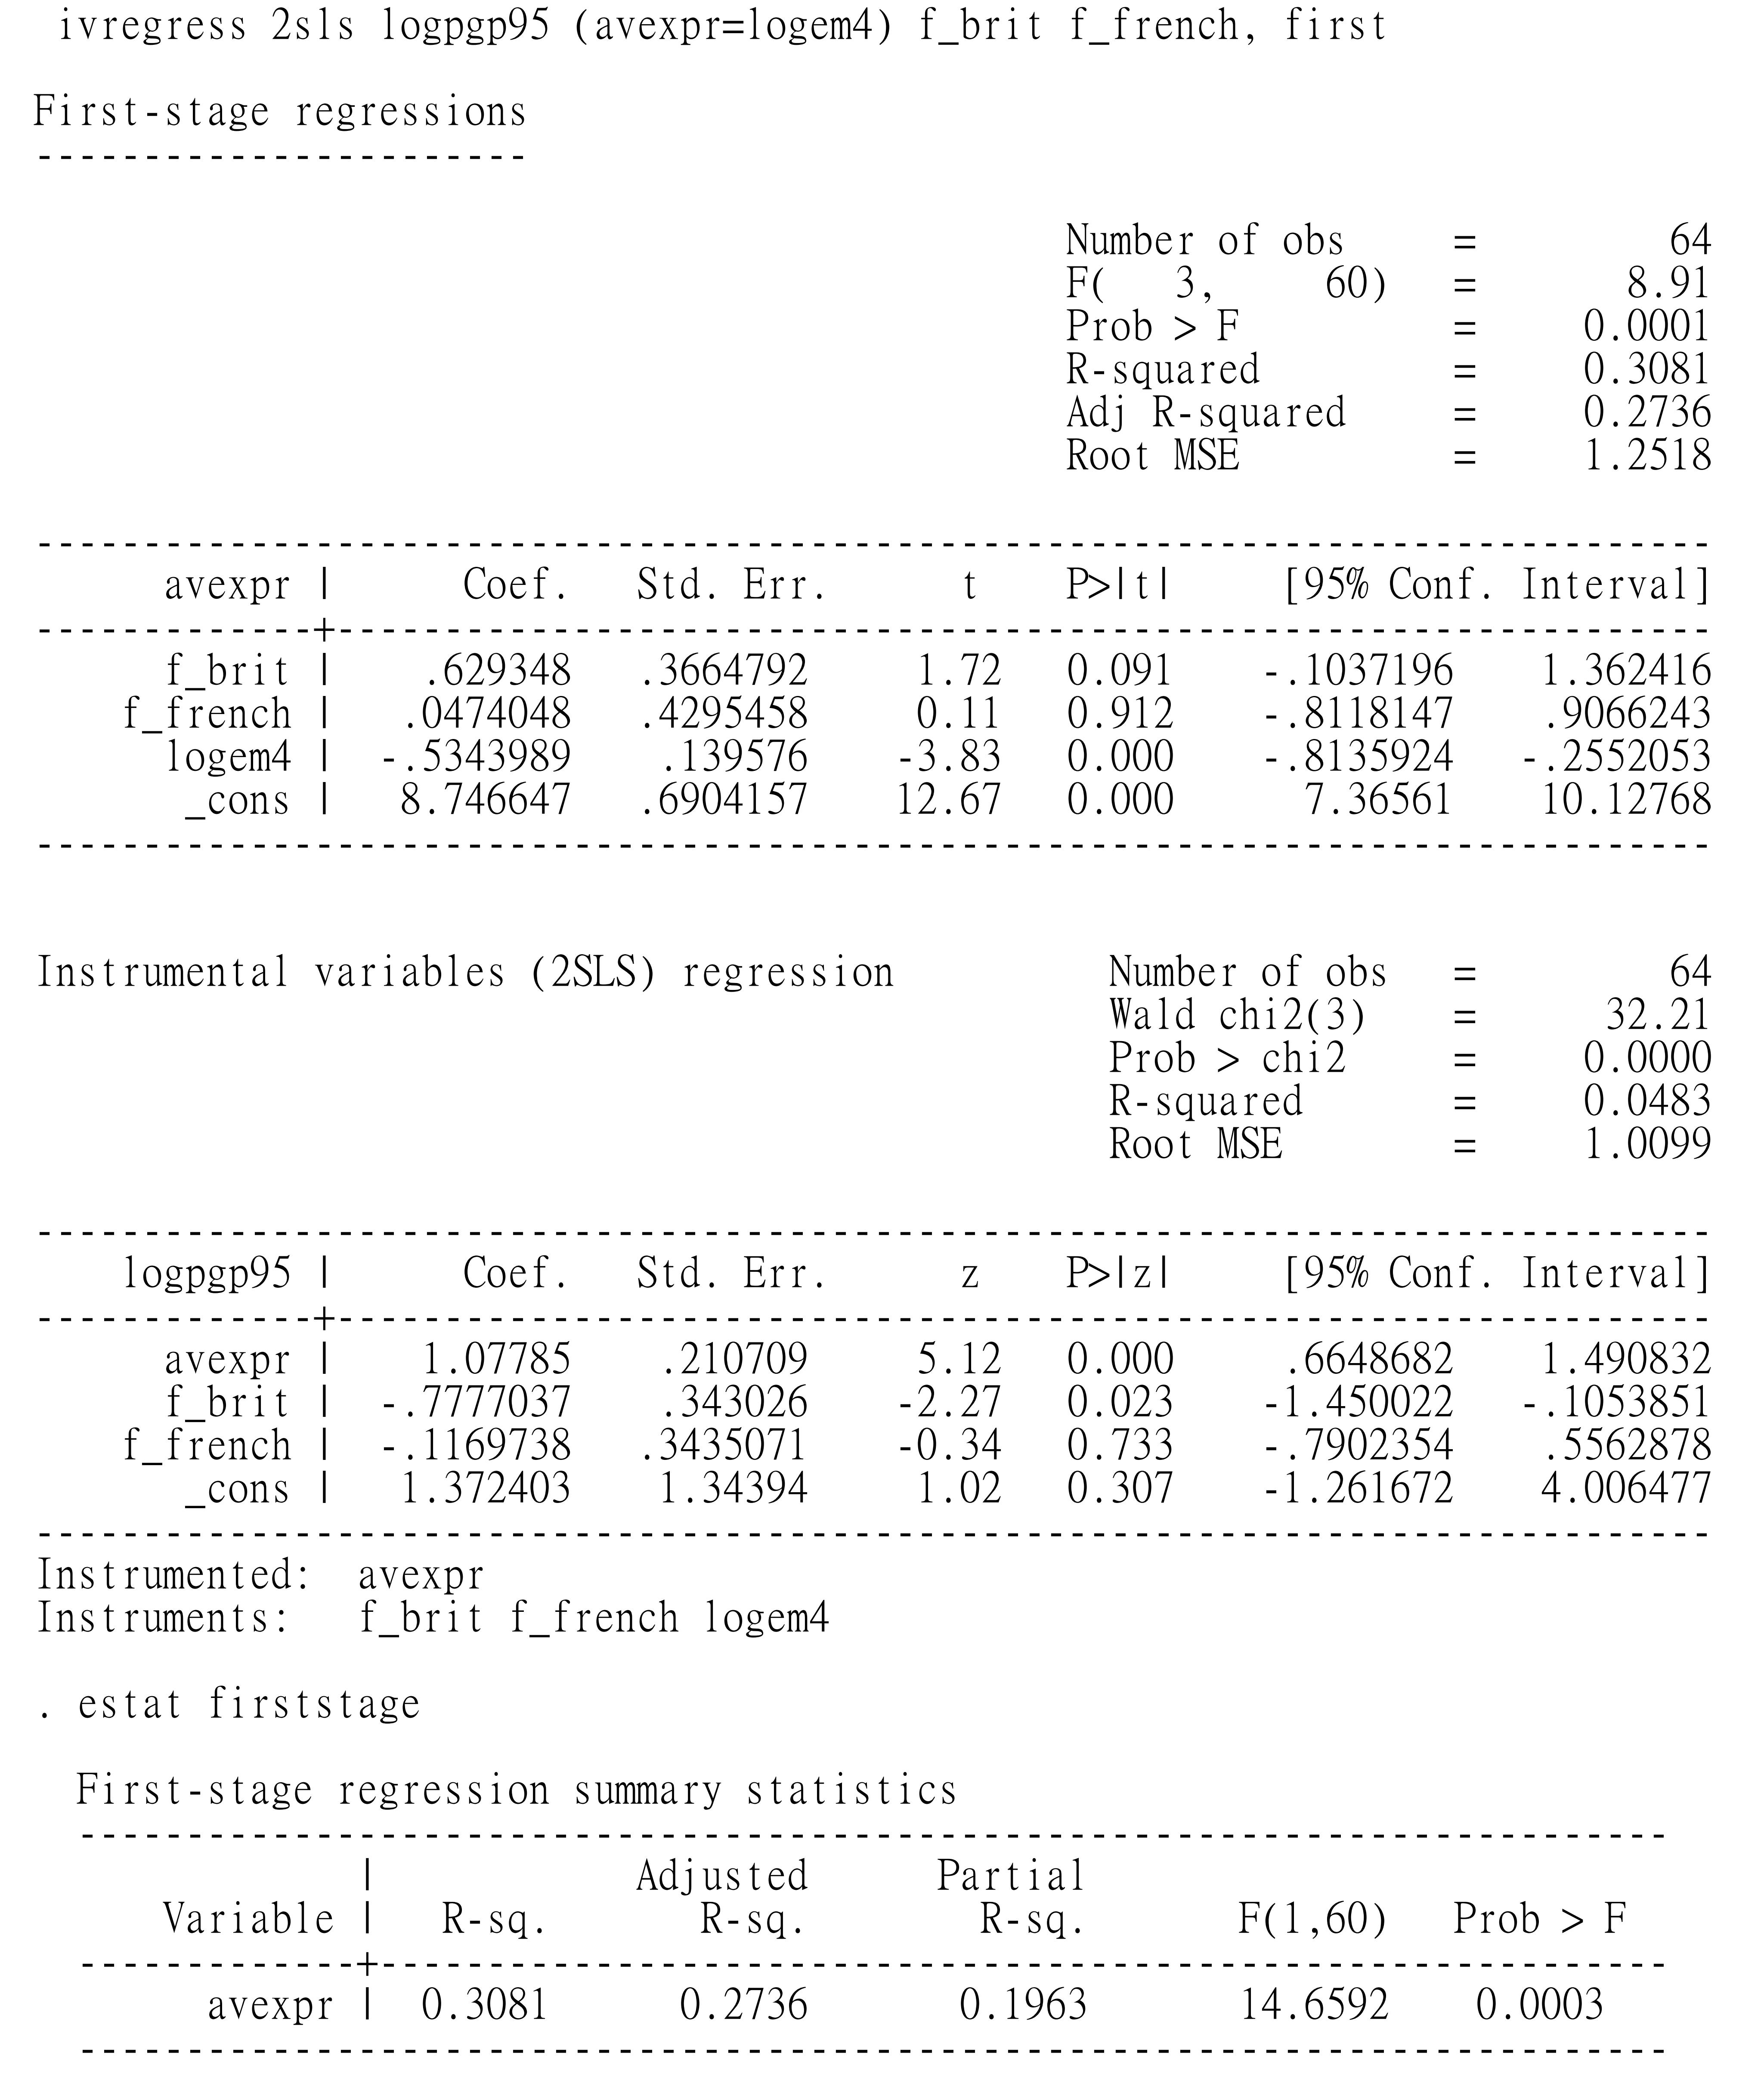
\includegraphics[width=0.6\textwidth]{figure/AJR_sta_t5_c1.jpg}
		\end{figure}
	\end{center}
\end{frame}



\begin{frame}[fragile]{STATA Command: ivreghdfe}
	\begin{itemize}
		\item Syntax:
\begin{lstlisting}
ivreghdfe depvar [controls] (endogenous_var = instruments) [if] [in] [weight], absorb(fixed effects) [options]
\end{lstlisting}
		
		\vspace{0.3cm}
		\item Example:
\begin{lstlisting}
ivreghdfe logpgp95 africa asia other_cont (avexpr=logem4), first
\end{lstlisting}
		
		\vspace{0.3cm}
		\item Basic structure:
		\begin{itemize}
			\vspace{0.2cm}
			\item \textbf{controls}: Exogenous control variables.
			\vspace{0.2cm}
			\item \textbf{endogenous\_var}: Endogenous variable(s) to be instrumented.
			\vspace{0.2cm}
			\item \textbf{instruments}: Instrumental variable(s).
		\end{itemize}
	\end{itemize}
\end{frame}



\begin{frame}{STATA Command: ivreghdfe}
	\begin{itemize}
		\item Key options:
		\begin{itemize}
			\vspace{0.2cm}
			\item \texttt{absorb(fixed effects)}: Specify fixed effects to control for (e.g., country, year).
			\vspace{0.2cm}
			\item \texttt{cluster()}: Cluster standard errors at a specified level.
			\vspace{0.2cm}
			\item \texttt{first}: Display first-stage regression results and diagnostics (optional).
		\end{itemize}
		
		\vspace{0.4cm}
		\item Advantages of \texttt{ivreghdfe}:
		\begin{itemize}
			\vspace{0.2cm}
			\item Handles multiple high-dimensional fixed effects efficiently.
			\vspace{0.2cm}
			\item Automatically clusters standard errors for valid inference.
			\vspace{0.2cm}
			\item Useful for large datasets and widely used in applied microeconometric research.
		\end{itemize}
	\end{itemize}
\end{frame}



\begin{frame}{Robustness Checks}
	\begin{itemize}
		\item Control for latitude
		\vspace{0.2cm}
		%\item Drop the four neo-Europes
		%\vspace{0.2cm}
		\item Maybe settler mortality just means bad disease environment
		\vspace{0.2cm}
		\begin{itemize}
			\item Can't control \textbf{life expectancy} because clearly this is endogneous (affected by treatment): \textbf{bad control}
			\vspace{0.2cm}
			\item Include measures of temperature and humidity meant to capture disease environment
			\vspace{0.2cm}
			\item Also put in measures of soil quality
		\end{itemize}
		\vspace{0.2cm}
		\item IV result survives all of these robustness checks
		
	\end{itemize}
\end{frame}






%\begin{frame}{Test Exclusion Restriction}
%	\begin{itemize}
%		\item According to their theory, settler mortality (M) affected settlements (S), settlements affected early institutions (C) and early institutions affected
%		current institutions (R)
%		\vspace{0.2cm}
%		\item Test whether any of
%		these variables, C, S, and M, has a direct effect
%		on income per capita, log y, 
%		\vspace{0.2cm}
%		\item Using measures of C and S as additional instruments
%		
%		
%		
%	\end{itemize}
%\end{frame}
%
%
%\begin{frame}{Test Exclusion Restriction}
%	\begin{itemize}
%		\item The TSLS estimates of the effect of protection against expropriation on GDP per capita using a variety
%		of instruments other than mortality rates
%		\vspace{0.2cm}
%		\item These estimates are always quite close
%		to those using settler mortality as IV
%		
%	\end{itemize}
%\end{frame}
%
%
%
%
%
%\begin{frame}{Test Exclusion Restriction}
%\begin{itemize}
%	\item Panel D adds the log of
%	mortality as an exogenous regressor
%	of instruments other than mortality rates
%	\vspace{0.2cm}
%	\item If mortality
%	rates faced by settlers had a direct effect
%	on income per capita, we would expect this
%	variable to come in negative and significant
%	
%\end{itemize}
%\end{frame}


\begin{frame}{Test of Exclusion Restriction}
	\begin{itemize}
		\item Theory:
				\vspace{0.3cm}
		\begin{itemize}
			\item Settler mortality (M) $\rightarrow$ Settlements (S) $\rightarrow$ Early institutions (C) $\rightarrow$ Current institutions (R) $\rightarrow$ Income ($\log y$).
		\end{itemize}
		\vspace{0.3cm}
		
		\item Exclusion restriction assumption:
				\vspace{0.3cm}
		\begin{itemize}
			\item Mortality (M) affects income ($\log y$) only through institutions (R).
		\end{itemize}
		\vspace{0.3cm}
		
	
	\end{itemize}
\end{frame}



\begin{frame}{Test of Exclusion Restriction}
	\begin{itemize}
	
		
		\item Testing strategy:
				\vspace{0.3cm}
		\begin{itemize}
			\item Test whether M, S, or C have a direct effect on $\log y$ after controlling for R.
					\vspace{0.3cm}
			\item Add log settler mortality directly as a regressor in the second stage.
		\end{itemize}
		\vspace{0.3cm}
		
		\item Result:
				\vspace{0.3cm}
		\begin{itemize}
			\item Mortality is not significantly related to income after controlling for institutions.
					\vspace{0.3cm}
			\item Supports the validity of the exclusion restriction.
		\end{itemize}
	\end{itemize}
\end{frame}



\begin{frame}{Test Exclusion Restriction}

\begin{center}
\begin{figure}[p]
	\centering
	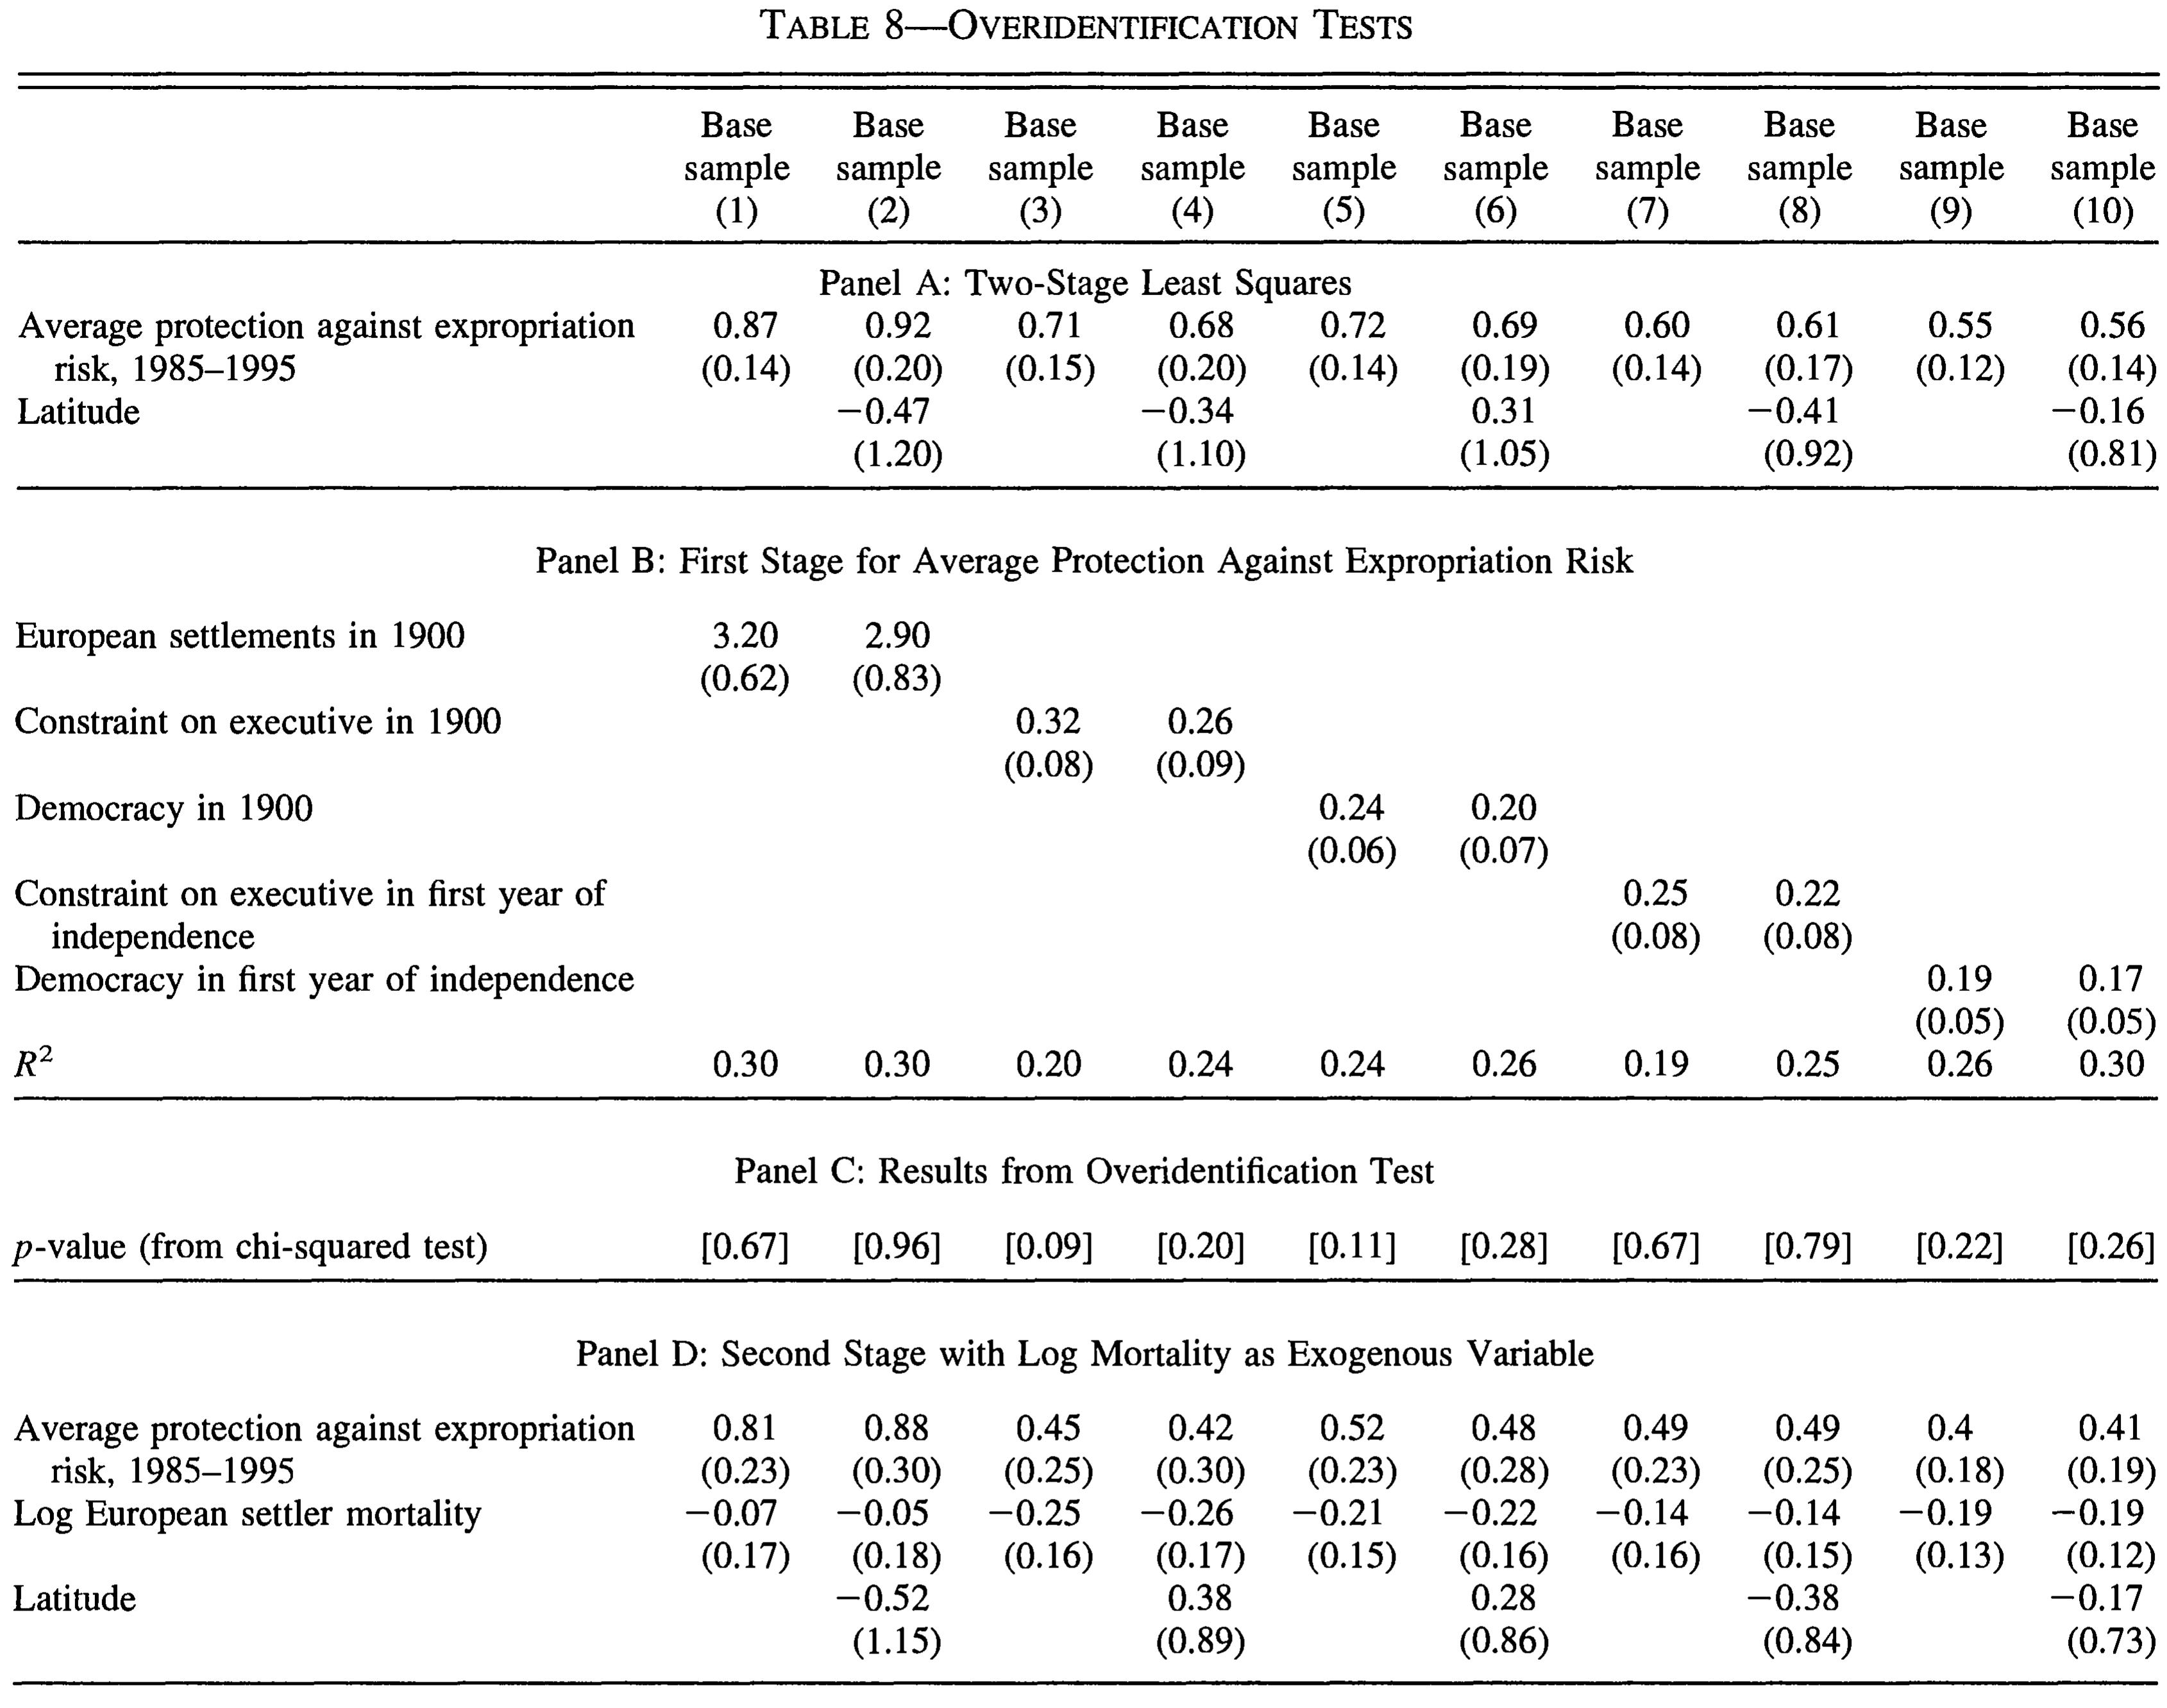
\includegraphics[width=0.8\textwidth]{figure/AJR_t8.jpg}
\end{figure}
\end{center}
\end{frame}









%\begin{frame}{Test Exclusion Restriction}
%\begin{itemize}
%\item So these results
%also show NO evidence that:
%\vspace{0.2cm}
%\begin{itemize}
%\item Mortality rates faced
%by settlers have a direct effect on income per capita
%\vspace{0.2cm}
%\item Mortality rates have an effect
%working through a variable other than institutions on income per capita
%\end{itemize}
%
%
%\end{itemize}
%\end{frame}




\title[]  
{R Example}


\author 
{}

%\institute{Institute of Economics, Academia Sinica  \\ Econ, NTU}
%\institute{Institute of Economics, Academia Sinica  \\ IMES/IDAS, NCCU}
\institute{}

%\author 
%{楊子霆 \\ 中研院經濟所}

%\institute 
%{中正大學國際經濟專題研討}




\date
{}


\begin{frame}{}
	\titlepage
\end{frame}





\begin{frame}{Overview}{Program and Data}
	\begin{itemize}
		
		\item See IV.R
		\vspace{0.2cm}
		\item Use AJR\_table4.dta
		

	
		
	\end{itemize}
\end{frame}



\begin{frame}[fragile]{Install Required Packages}
	\begin{itemize}
		\item Install and load required packages:
		\vspace{0.2cm}
\begin{lstlisting}
library(AER)       # for IV regression
library(haven)     # for reading Stata files
library(texreg)    # for regression tables
library(dplyr)     # for data manipulation
library(tibble)    # for rownames handling
library(xml2)      # for HTML processing
library(rvest)     # for HTML table extraction
library(writexl)   # for Excel output
\end{lstlisting}
		\vspace{0.2cm}
		\item \textbf{AER}: Implements instrumental variables regression
				\vspace{0.2cm}
		\item \textbf{texreg}: Creates publication-quality regression tables
				\vspace{0.2cm}
		\item \textbf{haven, dplyr, tibble}: Data import and manipulation
				\vspace{0.2cm}
		\item \textbf{xml2, rvest, writexl}: Convert and export results
	\end{itemize}
\end{frame}

\begin{frame}[fragile]{R Commands: ivreg}
\begin{lstlisting}
# Run IV regression
ivreg(logpgp95 ~ avexpr + lat_abst | logem4 + lat_abst, data = data)
\end{lstlisting}
	\begin{itemize}
		
		\vspace{0.2cm}
		\item \textbf{formula}: outcome ~ endogenous + exogenous | instruments + exogenous
		\vspace{0.2cm}
		\item \textbf{data}: specify the data frame
		\vspace{0.2cm}
		%\item Requires \textbf{AER} package: library(AER)
		%\vspace{0.2cm}
		\item Equivalent to STATA's \textbf{ivregress 2sls}
	\end{itemize}
\end{frame}

%\begin{frame}[fragile]{R Commands: texreg}
%	\begin{itemize}
%\begin{lstlisting}
%htmlreg(list(model1, model2), 
%file = "results.html",
%custom.model.names = c("Col1", "Col2"),
%custom.note = "Sample: Base",
%digits = 3)
%\end{lstlisting}
%		
%		\vspace{0.2cm}
%		\item \textbf{texreg} package offers three main functions:
%				\vspace{0.2cm}
%		\begin{itemize}
%			\item \textbf{htmlreg}: output to HTML
%					\vspace{0.2cm}
%			\item \textbf{texreg}: output to LaTeX
%					\vspace{0.2cm}
%			\item \textbf{screenreg}: output to console
%		\end{itemize}
%	\end{itemize}
%\end{frame}
%
%\begin{frame}[fragile]{R Commands: texreg}
%	\begin{itemize}
%		\item Main arguments:
%		\vspace{0.2cm}
%			\begin{itemize}
%		\item \textbf{list()}: list of model objects to include
%		\vspace{0.2cm}
%		\item \textbf{file}: output file path and name
%		\vspace{0.2cm}
%		\item \textbf{custom.model.names}: specify column names
%		\vspace{0.2cm}
%		\item \textbf{custom.note}: add table notes
%		\vspace{0.2cm}
%		\item \textbf{digits}: number of decimal places
%		\vspace{0.2cm}
%		\item \textbf{include.rsquared}, \textbf{include.nobs}: include R² and sample size
%			\end{itemize}
%	\end{itemize}
%\end{frame}
%
%\begin{frame}[fragile]{Converting Output Formats}
%	\begin{itemize}
%\begin{lstlisting}
%# Convert HTML to Excel/CSV
%table_data <- read_html("results.html") %>%
%html_table() %>%
%.[[1]]  # get first table
%
%# Save as Excel
%write_xlsx(table_data, "results.xlsx")
%
%# Save as CSV
%write.csv(table_data, "results.csv", row.names = FALSE)
%\end{lstlisting}
%		
%		\vspace{0.2cm}
%		\item Requires packages: \textbf{xml2}, \textbf{rvest}, \textbf{writexl}
%	\end{itemize}
%\end{frame}




\title[]  
{Practical Issues}


\author 
{}

%\institute{Institute of Economics, Academia Sinica  \\ Econ, NTU}
%\institute{Institute of Economics, Academia Sinica  \\ IMES/IDAS, NCCU}
\institute{}

%\author 
%{楊子霆 \\ 中研院經濟所}

%\institute 
%{中正大學國際經濟專題研討}




\date
{}


\begin{frame}{}
	\titlepage
\end{frame}


\begin{frame}{Practical Tips for IV Design}{Checking for Weak Instruments}
	\begin{itemize}
		\item[1.] Check IV relevance:
		\begin{itemize}
			\vspace{0.2cm}
			\item Is the instrument theoretically plausible?
			\vspace{0.2cm}
			\item Are the first-stage coefficients of the expected sign and reasonable magnitude?
			\vspace{0.2cm}
			\item Report the first-stage F-statistic for instrument strength.
		\end{itemize}
		\vspace{0.3cm}
		\item Rule of thumb:
		\begin{itemize}
			\vspace{0.2cm}
			\item If $F$-statistic > 10: Instruments are considered strong; TSLS is reliable.
			\vspace{0.2cm}
			\item If $F$-statistic < 10: Instruments are weak; TSLS may be biased.
		\end{itemize}
		\vspace{0.3cm}
		\item Consequences of weak instruments:
		\begin{itemize}
			\vspace{0.2cm}
			\item TSLS estimator becomes biased toward OLS.
			\vspace{0.2cm}
			\item Standard t-statistics and confidence intervals are invalid (non-normal distribution).
		\end{itemize}
	\end{itemize}
\end{frame}



\begin{frame}{Testing for Weak Instruments}
	\begin{itemize}
		\item \textbf{First-stage F-statistic} (homoskedastic case):
				\vspace{0.2cm}
		\begin{itemize}
			\item Standard F-test from first-stage regression
					\vspace{0.2cm}
			\item Compare to Stock-Yogo critical values
		\end{itemize}
		\vspace{0.2cm}
		
		\item \textbf{Kleibergen-Paap rk statistic} (heteroskedastic case):
				\vspace{0.2cm}
		\begin{itemize}
			\item Robust version of Cragg-Donald F-statistic
					\vspace{0.2cm}
			%\item Tests the rank condition when errors are not i.i.d.
			\item Still compare to Stock-Yogo critical values (though conservative)
		\end{itemize}
		\vspace{0.2cm}
		
		\item \textbf{Interpretation:} If test statistic $<$ critical value, instruments are likely weak, requiring robust inference methods.
	\end{itemize}
\end{frame}



\begin{frame}{Statistical Inference Robust to Weak Instruments}
	\begin{itemize}
		\item When instruments are weak (as identified by the previous tests), standard TSLS inference is invalid:
%		\begin{itemize}
%			\item Confidence intervals are too narrow
%			\item Hypothesis tests have incorrect size
%			\item Point estimates may be biased toward OLS
%		\end{itemize}
		\vspace{0.3cm}
		\item Alternative inference methods that remain valid with weak instruments:
		\begin{itemize}
			\vspace{0.2cm}
			\item \textbf{Anderson-Rubin test}:
			\vspace{0.2cm}
			\begin{itemize}
				\item Valid regardless of instrument strength
				%\vspace{0.2cm}
%				\item Tests the joint null hypothesis $H_0: \beta = \beta_0$ directly
%				\item Provides correct size even when instruments are arbitrarily weak
			\end{itemize}
			\vspace{0.2cm}
			\item \textbf{Weak IV robust confidence intervals}:
			\vspace{0.2cm}
			\begin{itemize}
				\item Construct confidence sets using methods that maintain correct coverage regardless of instrument strength (e.g., AR-based CI)
							\vspace{0.2cm}
				\item May be wider than conventional CI, reflecting the uncertainty from weak instruments
			\end{itemize}
		\end{itemize}
	\end{itemize}
\end{frame}





%
%\begin{frame}{Statistical Inference Robust to Weak Instruments}
%	\begin{itemize}
%		\item When instruments are weak, standard TSLS inference is invalid.
%		\vspace{0.3cm}
%		\item Alternative inference methods:
%		\begin{itemize}
%			\vspace{0.2cm}
%			\item \textbf{Anderson-Rubin test}:
%						\vspace{0.2cm}
%			\begin{itemize}
%				\item Valid even if instruments are weak.
%							\vspace{0.2cm}
%				\item Tests the joint null hypothesis without relying on first-stage strength.
%			\end{itemize}
%			\vspace{0.2cm}
%		%	\item \textbf{Kleibergen-Paap rk statistic}:
%		%				\vspace{0.2cm}
%		%	\begin{itemize}
%		%		\item Generalization of the Anderson-Rubin test under heteroskedasticity.
%	%		\end{itemize}
%			\vspace{0.2cm}
%			\item \textbf{Weak IV robust confidence intervals}:
%						\vspace{0.2cm}
%			\begin{itemize}
%				\item Construct confidence sets that are valid regardless of instrument strength (e.g., using robust AR CI).
%			\end{itemize}
%		\end{itemize}
%	
%	\end{itemize}
%\end{frame}




\begin{frame}{Statistical Inference Robust to Weak Instruments}
	\begin{itemize}
	
		\item Practical implementation using Stata:
		\begin{itemize}
			\vspace{0.2cm}
			\item \texttt{ivreghdfe} supports weak IV diagnostics.
						\vspace{0.2cm}
			\item Use the \texttt{first} option to obtain Cragg-Donald F-statistic and Anderson-Rubin tests
			%			\vspace{0.2cm}
			%\item Use the \texttt{ar} option to perform Anderson-Rubin tests robust to weak instruments.
		\end{itemize}
	\end{itemize}
\end{frame}





\begin{frame}{Statistical Inference Robust to Weak Instruments}
	
	\begin{center}
		\begin{figure}[p]
			\centering
			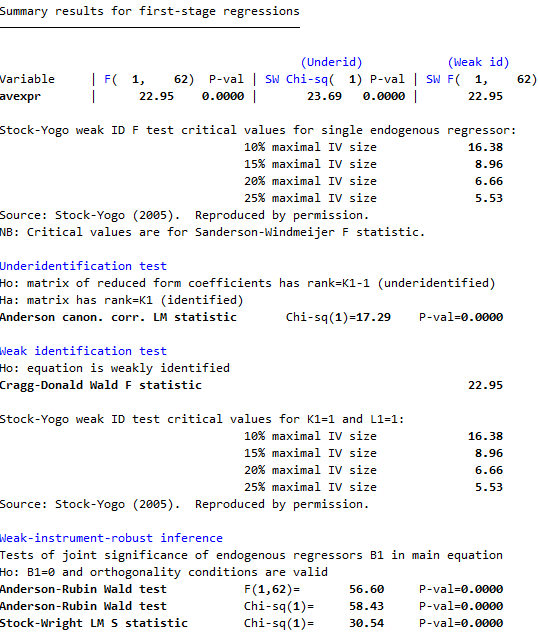
\includegraphics[width=0.5\textwidth]{figure/weak_iv_stata.png}
		\end{figure}
	\end{center}
\end{frame}





%\begin{frame}{Practical Tips For IV Design}
%	What are the consequences of weak instruments?	
%	\begin{align*}
%		& \hat{\alpha}_{TSLS}=\dfrac{Cov(Y_{i},Z_{i})}{Cov(D_{i},Z_{i})}
%	\end{align*}
%	\begin{itemize}
%		\item If $Cov(D_{i},Z_{i})$ is small, the small changes in $Cov(Y_{i},Z_{i})$ can induce big changes in $\hat{\alpha}_{TSLS}$
%		\vspace{0.2cm}
%		\item Suppose in one sample you calculate $Cov(D_{i},Z_{i})=0.00001$!
%		\vspace{0.2cm}
%		\item Therefore, from one sample to the next, $\hat{\alpha}_{TSLS}$ can change dramatically
%		\vspace{0.2cm}
%		\item Under this situation, the normal distribution is a poor approximation to the sampling distribution of $\hat{\alpha}_{TSLS}$
%		\vspace{0.2cm}
%		%\item A better approximation is that $\hat{\alpha}_{TSLS}$ is distributed as the ratio of two correlated normal random variables
%		%\vspace{0.2cm}
%		\item If instruments are weak, the usual methods of inference are unreliable - potentially very unreliable.
%	\end{itemize}
%\end{frame}



\begin{frame}{Practical Tips For IV Papers}
		\begin{figure}
		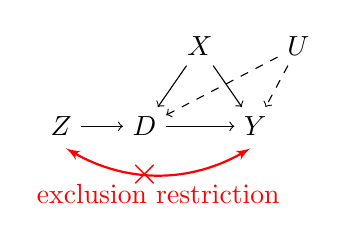
\begin{tikzpicture}[comment/.style={rectangle, text centered}]
			\centering
			\node (u) {$X$};
			\node (U) [right=2em of u] {$U$}; 
			\node (D) [below=1.5em of u, xshift=-2em] {$D$};
			\node (Z) [left=1.5em of D] {$Z$};
			\node (Y) [below=1.5em of u, xshift=2em] {$Y$};
			
			\draw [->,solid] (u) -- node [auto]{} (D);
			\draw [->,solid] (u) --  node [auto, swap]{} (Y);
			\draw [->,dashed] (U) -- node [auto, swap]{} (D);
			\draw [->,dashed] (U) -- node [auto]{}(Y);
			\draw [->] (D) -- node [auto]{} (Y);
			\draw [->] (Z) -- node [auto]{} (D);
			\draw[<->, >=latex', shorten >=2pt, shorten <=2pt, bend right=30, thick, color=red] 
			(Z.south) to node[auto, swap] {exclusion restriction}(Y.south);
			\node  [comment, below = 0.08 of D] (1) {\Large\color{red}$\times$};
		\end{tikzpicture}
	\end{figure}
	\begin{itemize} 
		\item[2.] Check exclusion restriction 
		\vspace{0.2cm}
		\item The exclusion restriction cannot be tested directly, but it can be falsified
		\vspace{0.2cm}
		\item \textbf{Placebo test} 
		\vspace{0.2cm}
		\begin{itemize}
			\item Test the reduced form effect of $Z_i$ on $Y_i$ in situations where it is impossible or extremely unlikely that $Z_i$ could affect $D_i$
			\vspace{0.2cm}
			\item Because $Z_i$ can't affect $D_i$, then the exclusion restriction implies that this placebo test should have zero effect.
		\end{itemize}
		
		%\item Nunn \& Wantchekon (2011): use distance to coast as an instrument for Africans, use distance to the coast in an Asian sample as falsification test
	\end{itemize}
\end{frame}

\begin{frame}{Practical Tips For IV Papers}
	\begin{itemize}
		\item[3.] If you have many IVs pick your best instrument and report the just identified model 
		\vspace{0.2cm}
		\item[4.] Look at the reduced form
		\begin{itemize}
			\vspace{0.2cm}
			\item Directly estimate the effect of instrument $Z$ on outcome $Y$
			\vspace{0.2cm}
			%\item The reduced form is estimated with OLS and is therefore unbiased.
			%\vspace{0.15cm}
			\item If you can't see the causal relationship of interest in the reduced form it is probably not there
		\end{itemize}
	\end{itemize}
\end{frame}




\begin{frame}{Suggested Readings}
	\begin{itemize} 
		\item Chapter 3, Mastering Metrics: The Path from Cause to Effect
		\vspace{0.2cm}
		\item Chapter 4, Mostly Harmless Econometrics
		\vspace{0.2cm}
		\item Chapter 7, Causal Inference: The Mixtape
	\end{itemize}
\end{frame}



\end{document} 